%%%%%%%%%%%%%%%%%%%%%%%%%%%%%%%%%%%%%%%%%%%%%%%%%%%%%%%%%%%%%%%%%%%%%%%%%%%%%%%%
%%%%%%%%%%%%%%%%%%   Vorlage für eine Abschlussarbeit   %%%%%%%%%%%%%%%%%%%%%%%%
%%%%%%%%%%%%%%%%%%%%%%%%%%%%%%%%%%%%%%%%%%%%%%%%%%%%%%%%%%%%%%%%%%%%%%%%%%%%%%%%

% Erstellt von Maximilian Nöthe, <maximilian.noethe@tu-dortmund.de>
% ausgelegt für lualatex und Biblatex mit biber

% Kompilieren mit
% latexmk --lualatex --output-directory=build thesis.tex
% oder einfach mit:
% make

\documentclass[
  oneside, % if not printed
  tucolor,       % remove for less green,
  BCOR=0mm,     % 12mm binding corrections, adjust to fit your binding % 0 if oneside
  parskip=half,  % new paragraphs start with half line vertical space
  open=any,      % chapters start on both odd and even pages
]{tudothesis}

\usepackage{subcaption}
% Warning, if another latex run is needed
\usepackage[aux]{rerunfilecheck}

% just list chapters and sections in the toc, not subsections or smaller
\setcounter{tocdepth}{1}

%------------------------------------------------------------------------------
%------------------------------ Fonts, Unicode, Language ----------------------
%------------------------------------------------------------------------------
\usepackage{fontspec}
\defaultfontfeatures{Ligatures=TeX}  % -- becomes en-dash etc.

% german language
\usepackage[main=english, ngerman]{babel}
%\setdefaultlanguage{english}

% for english abstract and english titles in the toc
%\setotherlanguages{german}

% intelligent quotation marks, language and nesting sensitive
\usepackage[autostyle]{csquotes}

% microtypographical features, makes the text look nicer on the small scale
\usepackage{microtype}

%------------------------------------------------------------------------------
%------------------------ Math Packages and settings --------------------------
%------------------------------------------------------------------------------

\usepackage{amsmath}
\usepackage{amssymb}
\usepackage{mathtools}

% Enable Unicode-Math and follow the ISO-Standards for typesetting math
\usepackage[
  math-style=ISO,
  bold-style=ISO,
  sans-style=italic,
  nabla=upright,
  partial=upright,
]{unicode-math}
\setmathfont{Latin Modern Math}

% nice, small fracs for the text with \sfrac{}{}
\usepackage{xfrac}


%------------------------------------------------------------------------------
%---------------------------- Numbers and Units -------------------------------
%------------------------------------------------------------------------------

\usepackage[
  locale=US,
  separate-uncertainty=true,
  per-mode=symbol-or-fraction,
  binary-units=true,
]{siunitx}
\sisetup{math-micro=\text{µ},text-micro=µ}
\DeclareSIUnit\gauss{G}

%\sisetup{round-mode=places,round-precision=2}
%------------------------------------------------------------------------------
%-------------------------------- tables  -------------------------------------
%------------------------------------------------------------------------------

\usepackage{booktabs}       % \toprule, \midrule, \bottomrule, etc

%------------------------------------------------------------------------------
%-------------------------------- graphics -------------------------------------
%------------------------------------------------------------------------------

\usepackage{graphicx}
\usepackage{grffile}
\usepackage{tabularx}

% allow figures to be placed in the running text by default:
\usepackage{scrhack}
\usepackage{float}
\floatplacement{figure}{htb}
\floatplacement{table}{htb}

% keep figures and tables in the section
\usepackage[section, below]{placeins}


%------------------------------------------------------------------------------
%---------------------- customize list environments ---------------------------
%------------------------------------------------------------------------------

\usepackage{enumitem}

%------------------------------------------------------------------------------
%------------------------------ Bibliographie ---------------------------------
%------------------------------------------------------------------------------

\usepackage[
  backend=biber,   % use modern biber backend
  autolang=hyphen, % load hyphenation rules for if language of bibentry is not
                   % german, has to be loaded with \setotherlanguages
                   % in the references.bib use langid={en} for english sources
  sorting=none,
  style=numeric,
]{biblatex}
\addbibresource{references.bib}  % the bib file to use
\DefineBibliographyStrings{german}{andothers = {{et\,al\adddot}}}  % replace u.a. with et al.

\usepackage{wrapfig}

% Last packages, do not change order or insert new packages after these ones
\usepackage[pdfusetitle, unicode, linkbordercolor=tugreen]{hyperref}
\usepackage{bookmark}
\usepackage[shortcuts]{extdash}

% yaml highlighting for the appendix
\usepackage{xcolor}
\usepackage{listings}

\usepackage{pdflscape}
\usepackage{afterpage}
\usepackage{typearea}
\usepackage{lipsum}
\usepackage{pdfpages}

\newcommand\YAMLcolonstyle{\color{red}\mdseries}
\newcommand\YAMLkeystyle{\color{black}\bfseries}
\newcommand\YAMLvaluestyle{\color{blue}\mdseries}

\makeatletter



% switch to key style at EOL
\lst@AddToHook{EveryLine}{\ifx\lst@language\language@yaml\YAMLkeystyle\fi}
\makeatother

\newcommand\ProcessThreeDashes{\llap{\color{cyan}\mdseries-{-}-}}

%------------------------------------------------------------------------------
%-------------------------    Angaben zur Arbeit   ----------------------------
%------------------------------------------------------------------------------

\author{Lukas Nickel}
\title{Stereo Reconstruction for the Early Days of CTA}
\date{2020}
\birthplace{Bielefeld}
\chair{Chair for Experimental Physics V}
\division{Faculty of Physics}
\thesisclass{Master of Science}
\submissiondate{20.04.2020}
\firstcorrector{Prof.~Dr.~Dr.~Wolfgang Rhode}
\secondcorrector{Prof.~Dr.~Bernhard Spaan}

% tu logo on top of the titlepage
\titlehead{
\includegraphics[height=1.5cm]{logos/tu-logo.pdf}}

\begin{document}
\frontmatter
\maketitle

% Gutachterseite
\makecorrectorpage

% hier beginnt der Vorspann, nummeriert in römischen Zahlen
\thispagestyle{plain}

\section*{Kurzfassung}
\begin{german}
In den letzten Jahrzehnten hat die $\gamma$-Astronomie 
viele Erkenntnisse über die Zusammensetzung des Universums gebracht.
Mitverantwortlich dafür waren die großen Image Air Cherenkov Telescope (IACT)
Experimente der dritten Generation.
In Zukunft soll diese Forschung begleitet und erweitert werden 
durch ein Experiment der nächsten Generation.
Das Cherenkov-Teleskope-Array (CTA) wird die Sensitiviät weiter steigern und den
beobachtbaren Energiebereich erweitern.
In dieser Arbeit werden Rekonstruktionsalgorithmen für CTA vorgestellt und Studien auf 
Monte-Carlo-Daten durchgeführt mit dem Fokus auf der frühen Phase des Experimentes.
Zu Beginn werden nur wenige Teleskope errichtet sein, sodass Ereignisse nur 
mit wenigen Teleskopen gesehen werden.
\end{german}

\section*{Abstract}
\begin{english}
In the past years the $\gamma$-astronomy has lead to many interesting
insights about the fundamental processes of the universe.
Part of that were the big imaging air cherenkov telescopes (IACTs) 
of the third generation.
In the future this research will be expanded with a next generation experiment.
The Cherenkov Telescope Array (CTA) will improve the sensitivity and
expand the observable energy range.
In this work we will present reconstruction algorithms for CTA und perform 
studies on monte carlo data with the focus on the early stages of the experiment.
In this stages CTA will only have some of the planned telescopes installed
leading to low multiplicity events.
\end{english}

%\setcounter{tocdepth}{6}
\tableofcontents

\mainmatter

% Hier beginnt der Inhalt mit Seite 1 in arabischen Ziffern
%\chapter{Gamma Astronomy V0.0}
\section{astro allgemein V0.1}
kurz halten, wenig aus dem bisherigen nehmen
kurze erwähnung von multi messenger, aber neutrinos und 
grav waves juckt uns eh nicht.
gammas pointen zur quelle, hadrons nicht
wir machen gammas!
ohne viel history
\section{gamma research, interessante physik V0.0}
\section{gamma entstehung V0.1}
entstehung gammas. mit kleinen erweiterungen schon da.
kurz: hadrons gibts auch. ist für uns background, weil mans auch misst
und es viel mehr gibt. gleichzeitig für den fall nicht so interessant.
\section{types of experiments, vor und nachteile V0.1}
direkt vs indirekt.
satelliten, tanks und iacts -> unterschiede/vorteile/nachteile.
Wir machen indirekt mit aicts.
\subsection{satelites V0.1}
\subsection{tanks V0.1}
\subsection{iacts V0.1}
\section{iacts V0.1}
\subsection{cherenkov licht, messen am boden V0.1}
\subsection{gamma shower V0.1}
\subsection{hadron shower V0.1}

\chapter{CTA V0.1}
sensitivity relativ zum crab für alle + cta angeben 
lst,mst,sst plots vielleicht text drum wrappen?
\section{current gen V0.1}
wir haben aktuell diese experimente:

sensitivity als crab flux ergänzen überall
\subsection{magic V0.1}
\subsection{veritas V0.1}
\subsection{hess V0.1}
\section{wie viel besser wird cta V0.1}
vergleich zu vorher: arrays auf beiden hemisphären, verschiedene teleskope, viele teleskope
status cta aktuell.
cta besonderheiten.
auflösungsrequirements unterbringen!
\subsection{lst V0.1}
passt grob
\subsection{mst V0.1}
passt grob
\subsection{sst V0.1}
passt grob

\chapter{Methods: Relativ allgemein V0.1}
wie werden daten genommen?
\section{Coordinate Frames V0.1}
wichtig, vor allem altaz, camera, nominal, ground
\section{Monte carlo V0.1}
ist wichtig duh
\subsection{corsika V0.1}
atmosphäre
\subsection{simtel V0.0}
telescope response
\section{ctapipe V0.1}
was ist das, warum ist das und was habe ich gemacht?
-> neu: num islands, fact cleaning
\subsection{telescope level  V0.1}
damit wir damit arbeiten können, muss erstmal kram gemacht werden, den
wir mal preprocessing nennen.
ctapipe ist nicht fertig, daher machen wir eigenen kram -> kai auf basis von ctapipe
liste der steps im detail.
\subsection{array level V0.1}
das sind so sachen wie energie, typ, richtung.
\section{Additional apporaches V0.1}
\subsection{disp methode, mono wie stereo V0.1}
\subsection{classification V0.1}
\subsection{machine learning V0.1}


\chapter{Analysis: Methods spezifiziert für unser Problem! V0.0}
mit zuvor erklärten methoden zusammen fassen was getan wird
\section{preprocessing  and used data V0.1}
erhaltene features hier oder dadrunter?
\subsection{telescope level V0.1}
\subsection{array level V0.1}
\section{high level alternative V0.0}
\subsection{gamma hadron sep V0.1}
machen wir auch per random forest 
\subsection{DISP V0.1}
random forest
median und iterative
\subsection{mono modell? V0.0}
wenn zeit ist als vergleich bei multi 2\&3
-> vlt machen die core und hmax schätzungen das da tatsächlich schlechter?

\chapter{Results V0.0}
\section{gamma/hadron V0.0}
\section{position mono V0.0}
\section{position stereo V0.0}
\section{position stereo cut V0.0}
\section{position stereo ohne hillas features, optimized for multi 2 ? V0.0}

\chapter{Conclusion V0.0}

\chapter{Gamma Astronomy}

\section{The Field of Astroparticle Physics}

The ballon flights of Victor Hess \cite{Hess:1912srp} are
often times cited as the starting point of astroparticle physics,
because they gave reason to believe, that the measured ionizing
radiation is of extraterrestrial origin. 

The radiation was referenced as "Höhenstrahlung" 
(see e.g. \cite{myssowsky1926versuche}) 
and "cosmic rays" (see e.g. \cite{millikan1928origin}) with 
the english term cosmic rays eventually winning out.

Soon after, in 1933, Carl D. Anderson discovered the existence
of antimatter using a cloud chamber \cite{PhysRev.43.491},
which is crucial for the measurement of especially
high energy photons.

Later years brought the discovery of several new particles,
that are imperative to modern astronomy:
pions \cite{LATTES1947}, muons \cite{PhysRev.52.1003}
and neutrinos \cite{Cowan103}.

Recently, the so far last discovery on this journey
was made with the measurement of the first gravitational 
waves \cite{PhysRevLett.118.221101}.

This leaves the field of astronomy with four different
messengers, which coins the term
multi messenger astronomy:
\begin{enumerate}
	\item Electromagnetic radiation
	\item Cosmic rays
	\item Neutrinos
	\item Gravitational waves
\end{enumerate}

Figure \ref{fig:multi_messenger} illustrates the key differences between
photons, protons and neutrinos.
This thesis focuses on the detection of cosmic and gamma rays.

\begin{figure}
	\centering
	\captionsetup{width=0.9\linewidth}
	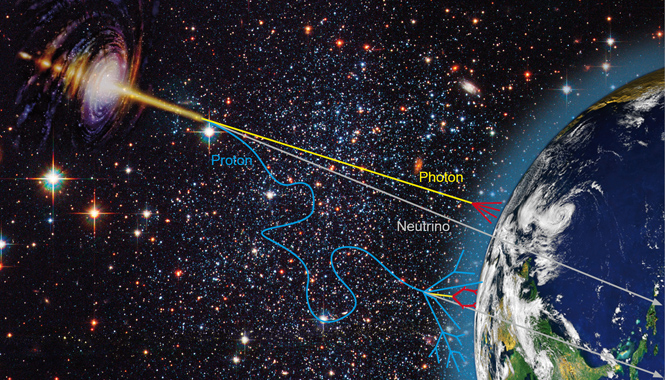
\includegraphics[width=0.9\textwidth]{images/astro-web-titel.jpg}
	\caption{Visualization of the behaviors of different messengers
		particles in modern astronomy.
		Photons and neutrinos travel through the universe without deflection,
		because they do not carry an electric charge.
		Neutrinos interact less than photons,
		which leads to a high proportion passing through earth.
		Charged cosmic rays get deflected by interstellar
		magnetic fields and thus generally do not allow for a reconstruction
		of the source position.
		The image is taken from the DESY-website at \cite{desy_mm_astro}.
	}
	\label{fig:multi_messenger}
\end{figure}

In contrast to charged cosmic rays, $\gamma$-rays point towards
their sources, allowing to search for bright sources of radiation.
This makes it possible to learn more about the acceleration processes
and sources, that produce high energy gamma and cosmic rays.
Two important classes of proposed sources are active galactic nuclei,
which are considered massive black holes, that produce jets and 
supernove remnants. (mehr research)

Researching the diffuse component of gamma-rays on the other hand holds
potential to find out more about interstellar magnetic fields and the
propagation of relativistic particles in the universe.

Another motivation to research gamma-rays lies in the assumption, that
dark matter could annihilate to photon pairs. (quelle im tu netz öffnen)

Due to the way gamma-rays are being detected, it is not possible
to avoid measuring cosmic rays as well.
At the same time cosmic rays are much more numerous,
which makes them the dominant background in gamma astronomy \cite{funcray}.

\section{Production of Gamma-Rays}
Creation of high-energy gamma-rays can not happen thermally,
but happens in a combination of high energy charged particles 
and interstellar targets or magnetic fields \cite{funcray}.
A model for the production at the source, the Self Synchroton Comptoon model,
focuses on photon emission from an initial pure electron distribution.
The key aspects of this model are now briefly presented. 

\textbf{Synchroton Radiation}

Propposed sources of cosmic and gamma rays include 
high magnetic fields. Any moving charged particle will thus be
deflected perpendicular to its moving direction
due to the Lorentz-force, forcing them on a radial trajectory.
At the same time a relativistic charged particle, 
that gets accelerated radially, emits synchroton 
photons with average energy given by:

\begin{equation}
	\langle E_{\gamma} \rangle \propto \frac{1}{M_P} E_P^2 B^2.
	\label{eq:synchroton}
\end{equation}

Here, $M_P$ and $E_P$ denote the accelerated particle's 
mass and energy respectively. With the inverse mass dependency 
it is immediately evident that
synchroton radiation plays a major role in leptonic 
emission and much less in hadronic emission.

A direct result of this is, that the electrons energy gets reduced
in the process, affecting ("cooling") the initial electron distribution.
This is sometimes referred to as synchroton cooling.

The emitted synchroton spectrum needs to be further modified 
if the emitting region is optically thick and photons 
get absorbed by the medium.
This is in fact always the case, as the regions contains 
both magnetic fields and a high density of electrons.

\textbf{Inverse Compton Scattering}
In a classical particle interpretation photons and electrons 
can collide exchanging energy and altering their directions.
For the normal case of Compton scattering the electron 
is assumed to be at rest and the photon can never gain 
energy by colliding with the electron.
This can be 
seen by the increase in wavelength in \eqref{eq:compton},
with $\lambda^{\prime}$ denoting the scattered photons 
wavelength, $\lambda$ denoting the initial photons wavelength  
and $\Theta$ denoting the scattering angle.

\begin{equation}
	\lambda^{\prime} - \lambda  \propto \left(1-\cos{\Theta} \right)
	\label{eq:compton}
\end{equation}

If the electron itself is moving with much higher energy
than the photon, this changes and the photon can gain substantial energy.
This is reffered to as inverse Compton scattering.
In that case, transforming the equations to the 
electron's frame of reference and back to the laboratory frame of reference
boosts the photons energy by a factor $\gamma$ for each transformation, 
with $\gamma$ being the Lorentz factor of the electron.

A limit to the photon energies is set by the scattering cross
section, which reduces with higher photon energies.
For low energies the cross section can be approximated by 
the Thomson cross section, for high energies
one uses the Klein-Nishina cross section. (quellen angeben)

The Synchroton Self Compton model combines the above mentioned
effects to produce a photon energy distribution from an
electron distribution, which is often times assumed to
follow a power-law spectrum initially.
The free parameters of the model can be interpreted as 
three frequencies: The minimum injection frequency $\nu_m$, 
the cooling frequency $\nu_c$ and the self-absorption frequency $\nu_a$.
Depending on the order of these parameters, different 
photon distributions can be generated.

A detailed analysis of the influence of the parameters of
the Synchroton Self Compton model, can be found in 
\cite{10.1093/mnras/stt1461}.


\section{Experiments for Cosmic and Gamma Rays}
Emitted $\gamma$-rays can be observed either directly
from outside the atmosphere via satellites or indirectly
via ground based gamma astronomy.

The different types of experiments differ in the way particles are detected and
the resulting energy ranges, where they are most sensitive.

\subsection{Satellite Experiments}
Satellite experiments allow direct measurements of gamma and cosmic rays, because of the operation
above the atmosphere.
This allows to use similar techniques as experiments located at terrestrial 
particle detectors: Incoming photons hit an initial layer and produce an electron pair 
via pair production. The tracks of these particles get observed before they reach the calorimeter,
where their energies get measured.

Despite the advantages over ground based experiments, the small detector areas 
limit the sensitivities at higher energies.

A currently operating example is the FERMI Gamma-ray Space Observatory (FGST) \cite{Atwood_2009}.
The Large Area Telescope (LAT) on 
the FGST covers an energy range of
\SI{20}{\mega\electronvolt} to \SI{100}{\giga\electronvolt} \cite{Atwood_2009}.
It is able to cover a huge field ov view (fov) of 
\SI{20}{\degree}. A second detector, the Gamma-ray Burst Monitor,
searches for gamma ray bursts using a scintilator setup to notify other experiments.

\subsection{Imaging Air Cherenkov Telescopes (IACTs)}
A class of ground-based observatories are the 
Imaging Air Cherenkov Telescopes (IACTs),
which will be the focus of this thesis.

In constrast to the satellite experiments, they cannot directly
observe the cosmic particle. Instead they use the atmosphere as detector medium.
High energy primary particles generate a cascade of secondary particles
when interacting with the atmosphere. These particles generate cherenkov
light, which is recorded by the IACTs.

Modern experiments include 
MAGIC \cite{ALEKSIC2012435},
VERITAS \cite{WEEKES2002221}
and HESS \cite{vincent2005hess},
all of which consist of multiple telescopes to observe the shower 
from different angles to improve the reconstruction.

The observable energy range generally generally lies in the range of
some \SI{10}{\giga\electronvolt} to some 10-\SI{100}{\tera\electronvolt}.

\subsection{Air Shower Arrays}
Air shower arrays, like IACTs, operate on the ground and thus also have 
to measure the particle indirectly.

In contrast to IACT-experiments, air shower arrays consist of a huge
number of single scintillation detectors, spaced on a grid on the ground.
Instead of the cherenkov light, they measure the
remaining particles of the shower. This makes them feasible
for energies even above the ones measured by IACTs.

A modern experiment is the High Altitude Water Cherenkov Observatory (HAWC) \cite{2015ICRC...34..966S}.
It uses \num{300} water tanks to measure air showers with a lower threshold
of under \SI{1}{\tera\electronvolt}.

\section{Detection of Gamma Rays with IACTs}
% \subsection{Detecting Gamma Rays}
\label{sec:measuring}

The primary particles of gamma or cosmic rays cannot be 
observed with IACTs directly. Instead one can measure the secondary particles
that emerge from the particles interaction with matter.

If the primary particle energy is high enough, the resulting 
secondary particles can interact with the atmosphere themself, thus starting a 
cascade of secondary particles.
Particles, that have enough energy, are faster than the local speed of light.
Because the electrons carry a charge and the air acts as dielectricum, 
cherenkov light gets emitted \cite{quelle suchen}.

Cherenkov photons get collected by the mirror(s) of a telescope
and projected onto a camera system mounted above the mirror.
Figure \ref{fig:iact_mirror_camera} illustrates the measurement of 
an air shower.

\begin{figure}
	\centering
	\captionsetup{width=0.9\linewidth}
	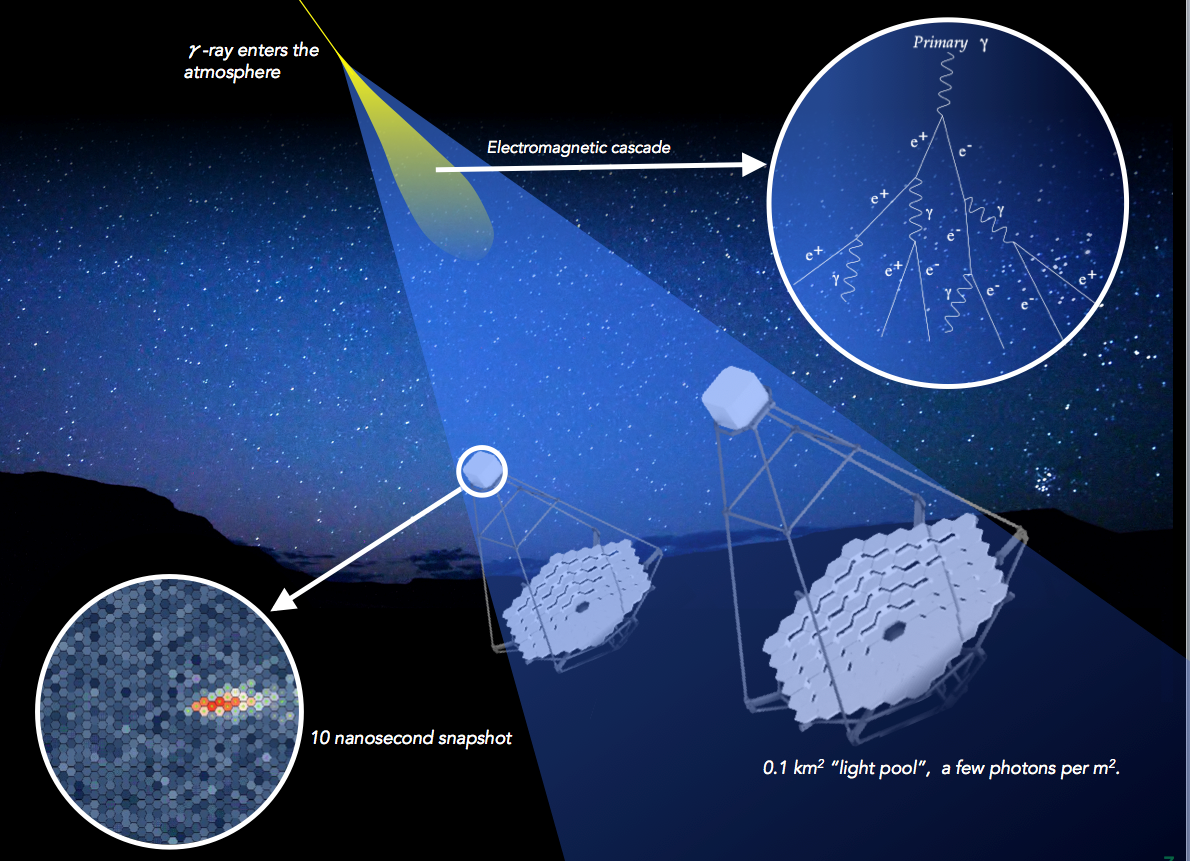
\includegraphics[width=0.9\textwidth]{images/cta47.png}
	\caption{A schematic illustration of the working principles of 
	an IACT experiment:
	A $\gamma$-ray produces an air shower in the atmosphere
	that points roughly towards the telescopes.
	Cherenkov light from the air shower 
	hits the mirrors and gets focused into a camera mounted on top.
	An illustration of the resulting image after integrating 
	\SI{10}{\nano\second} of the pixel measurements
	can be seen in the left bottom corner.
	The image is taken from the CTA-website \cite{cta_web}.}
	\label{fig:iact_mirror_camera}
\end{figure}

Depending on whether the primary particle is 
a photon/electron or a heavier, hadronic particle such as a proton 
or iron core, the interactions in the atmosphere and the 
produced secondary particles vary.

This leads to a separation of electromagnetic and hadronic showers.
If the experiment is primarly looking for 
gamma rays, e.g. if measuring a known source like the Crab Nebula, 
the hadronic showers act as dominant background.
As hadronic showers get observed much more frequently, 
the identification of the primary particle type is a very important 
task, often times referred to as gamma-/hadron-separation.

\subsection{Electromagnetic Showers in the Atmosphere}
Electromagnetic showers consist mainly of two types of particles:
\begin{enumerate}
	\item{Photons $\gamma$}
	\item{Electrons $e^-$ / Positrons $e^+$}
\end{enumerate}

The main interaction for high energy photons is pair 
production, generating an $e^+/e^--$pair where the summed energy of 
the lepton pair equals the photon energy.
On the other hand high energy electrons lose 
most of their energy by radiating bremsstrahlung, leading to a photon with 
an energy close to the electron energy.
Only at lower particle energies other interaction forms show their impact,
with particle scattering and ionization 
leading to more continuous energy losses.

These assumptions lead to the most basic model of an 
electromagnetic shower, proposed by Bhabha and Heitler in 1937
\cite{doi:10.1098/rspa.1937.0082}.
It starts with a high energy primary photon before its interaction in the atmosphere 
and continues the calculation in discrete epochs.
The photon produces a pair of $e^-$ and $e^+$ in the first epoch.
Because of the high energies at play, the direction of these secondary 
particles does not deviate significantly from the photon's direction, 
making the problem essentially one-dimensional.
The $e^+/e^-$ continue on to radiate a photon each and the cycle continues.
Each step doubles the number of particles in the shower with each particle 
on average getting half the energy of its parent particle.
These processes continue until the energy of the $e^+/e^-$ becomes low enough for
continuous ionization processes to become relevant.
At this point the particle is considered to be stopped and the shower
does not evolve further.

Today monte carlo calculations get used to simulate the properties 
of particle showers in the atmosphere.
The most common software to model the atmospheric interactions is
CORSIKA \cite{Engel:2018akg}.

Figure \ref{fig:gamma_shower} illustrates the Bhabha-Heitler model (left)
and a \SI{100}{\giga\electronvolt} gamma shower, simulated with CORSIKA (right).

\begin{figure}
	\centering
	\captionsetup{width=0.9\linewidth}
	\begin{subfigure}{.7\textwidth}
  		\centering
  		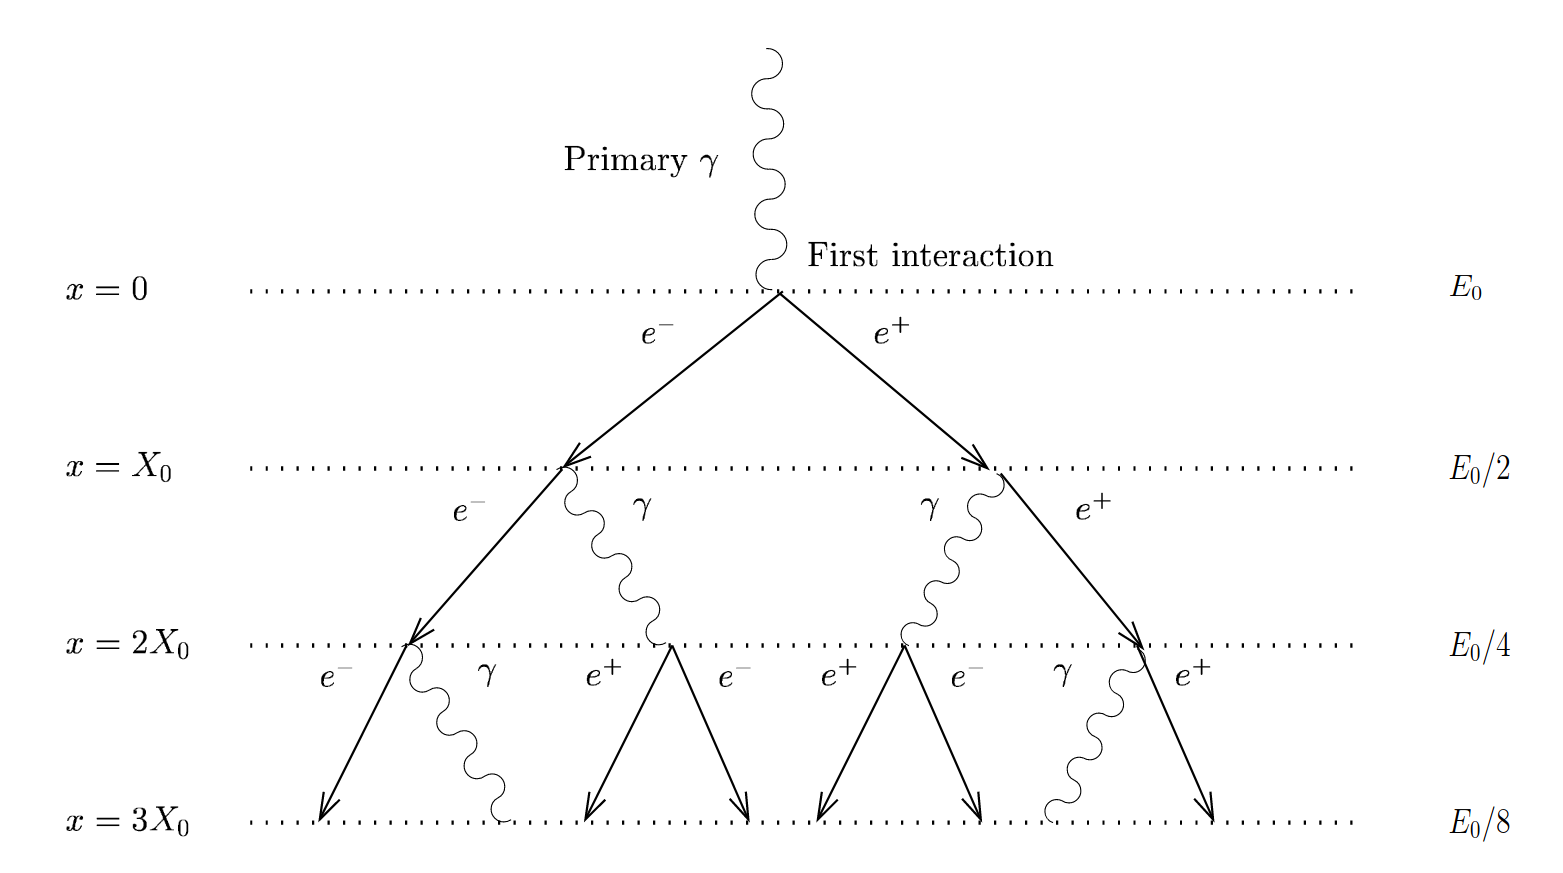
\includegraphics[width=\linewidth]{images/em_shower_illustration.png}
	\end{subfigure}%
	\begin{subfigure}{.2\textwidth}
 		\centering
		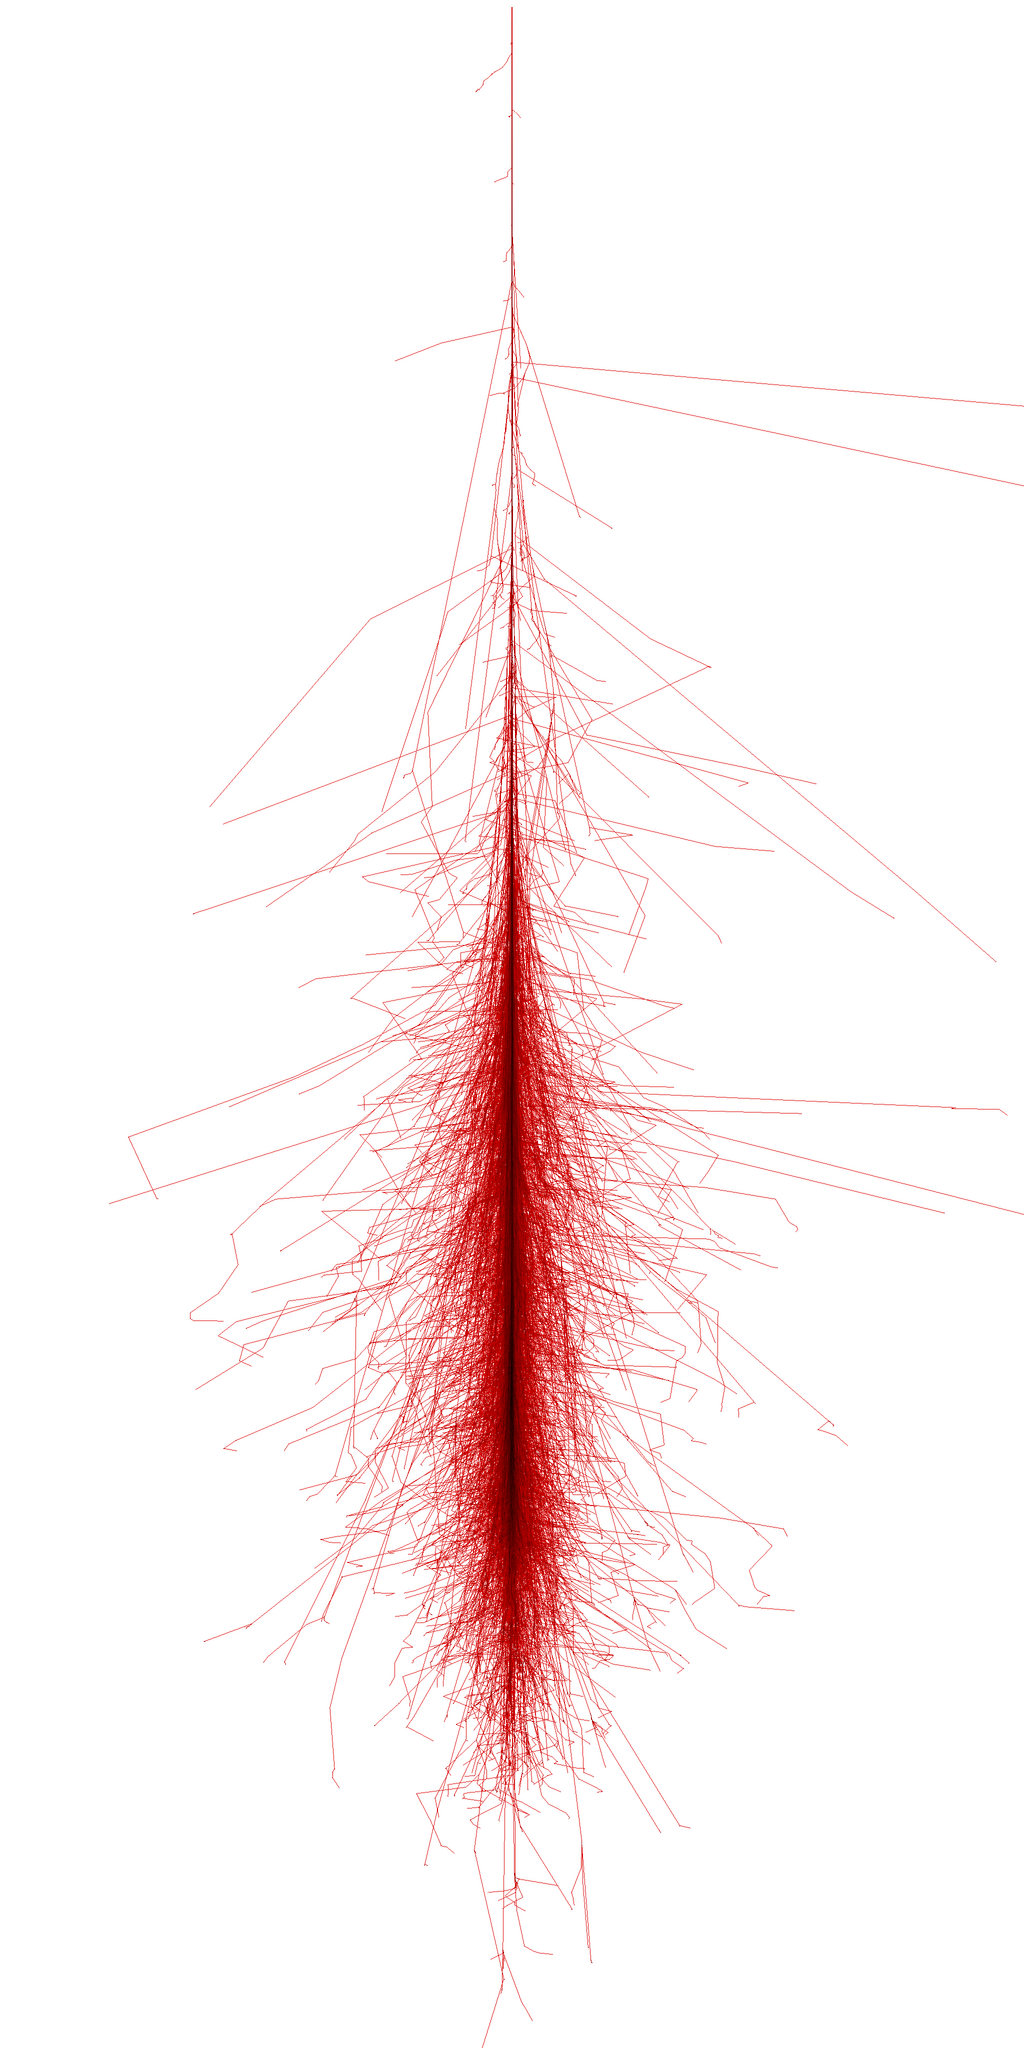
\includegraphics[width=\linewidth]{images/corsika_100gev_photon.png}
	\end{subfigure}
	\caption{
		Left: A schematic illustration of the first epochs of the 
		Bethe-Heitler shower model with equal radiation lengths for
		bremsstrahlung and pair production.
		The image is taken from an inaugural thesis 
		by Stefan Funk \cite{funk_doctor}. \\
		Right: A \SI{100}{\giga\electronvolt} gamma-shower as xz-projection, simulated with CORSIKA.
		The shower is relatively contained with only little extent perpendicular 
		to the shower direction (z-axis). The image is taken from 
		the CORSIKA-website \cite{corsika_showers}}
	\label{fig:gamma_shower}
\end{figure}

\subsection{Hadronic Showers in the Atmosphere}
Hadronic showers include all the interactions known from 
electromagnetic showers, but add nuclear interactions on top.
These lead to non-negligible additional energy losses 
and the creation of secondary hadronic particles.

Approximations are more difficult to do and monte carlo simulations 
become the only way to reasonably calculate shower behavior.

At the end of the shower a relevant portion of the particles have decayed into the 
lightest hadronic particles, pions ($\pi^0, \pi^+, \pi^-$), of which the neutral pions 
rapidly decay into photons.
This means that a part of the hadronic shower
eventually becomes an electromagnetic subshower.

Figures \ref{fig:proton_shower}
shows some of the particles generated in a hadronic shower (left)
and a \SI{100}{\giga\electronvolt} proton shower, simulated with CORSIKA (right).

\begin{figure}
	\centering
	\captionsetup{width=0.9\linewidth}
	\begin{subfigure}{.7\textwidth}
  		\centering
  		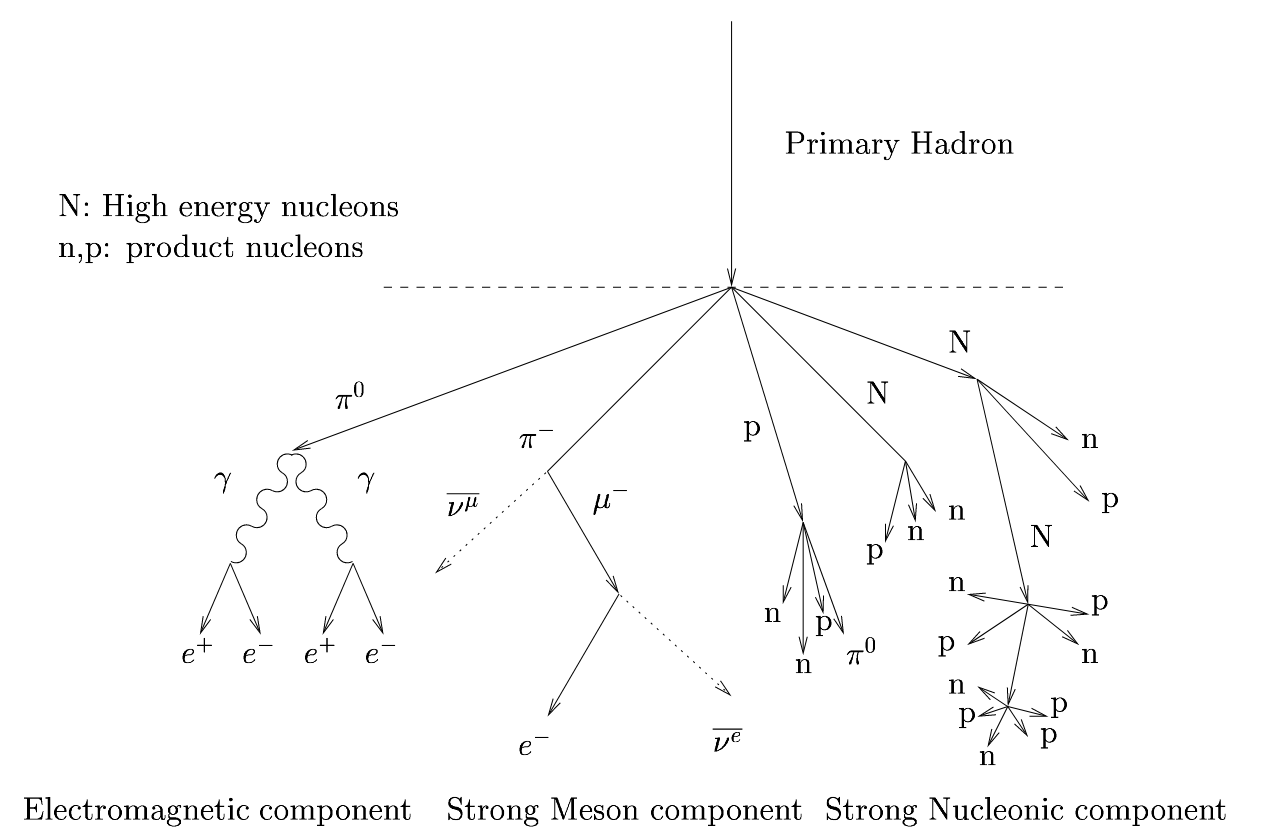
\includegraphics[width=\linewidth]{images/hadron_shower_illustration.png}
	\end{subfigure}%
	\begin{subfigure}{.2\textwidth}
 		\centering
		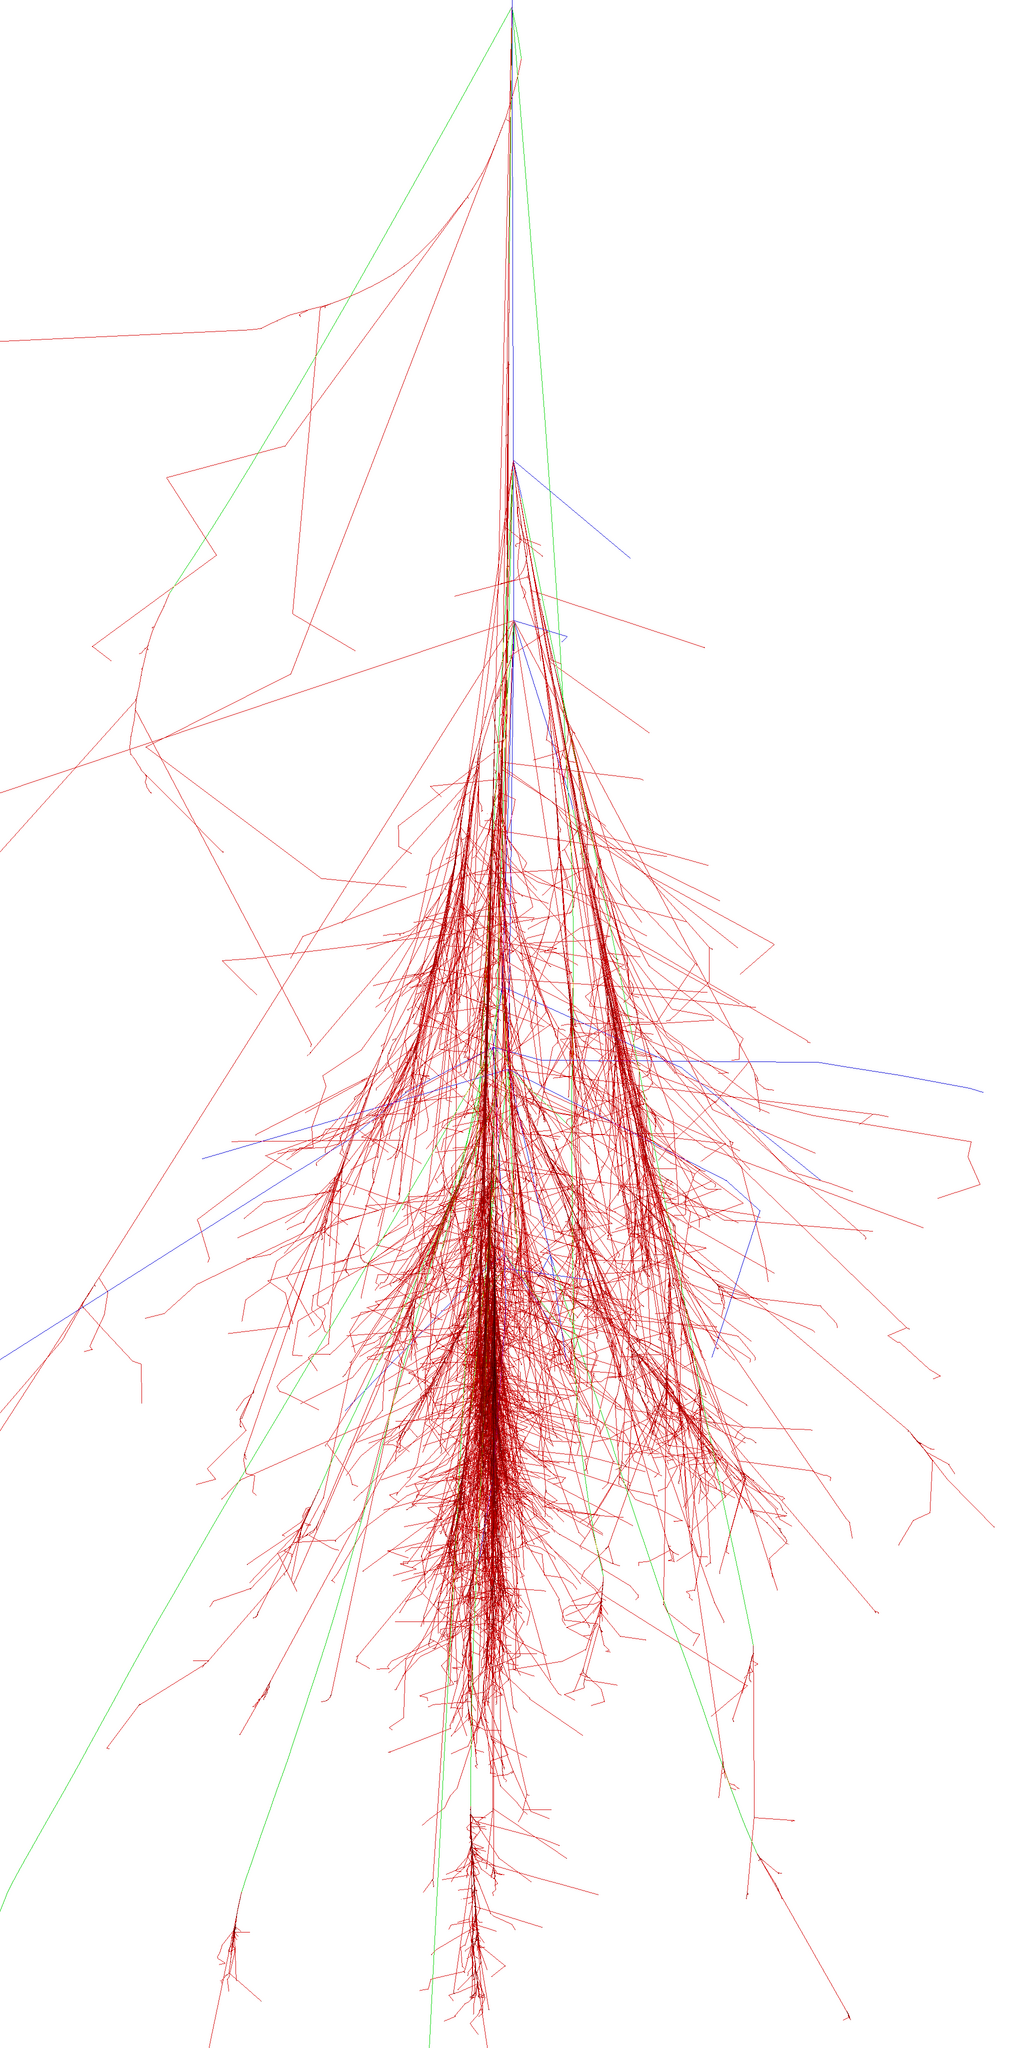
\includegraphics[width=\linewidth]{images/corsika_100gev_proton.png}
	\end{subfigure}
	\caption{
		Left: A purely qualitative,
		schematic illustration of the generation of a hadronic shower.
		It shows how the primary hadron generates different subshowers
		with vastly different particles.
		The image is taken from an inaugural thesis 
		by Stefan Funk \cite{funk_doctor}.\\
		Right: A \SI{100}{\giga\electronvolt} proton-shower as xz-projection,
		simulated with CORSIKA.
		The shower is less contained than the gamma shower of equal energy in 
		figure \ref{fig:gamma_shower}.
		Different colors indicate different particle types.
		The image is taken from 
		the CORSIKA-website \cite{corsika_showers}.}
	\label{fig:proton_shower}
\end{figure}





% \chapter{IACT Experiments}
\label{cta}

sensitivity in crab flux angeben

\section{The Current Generation}

Towards the end of the 1990s several third generation experiments were
proposed:
H.E.S.S and MAGIC, deriving from parts of the HEGRA collaboration, 
VERITAS from Whipple and the no longer operating CANGAROO from Adelaide and 
several japanese universities \cite{HILLAS201319}. All of these
were designed as stereoscopic imaging telescopes building on the progress made during the 
earlier experiments with two experiments located on each the north and the south hemisphere.

\subsection{Major Atmospheric Gamma Imaging Telescopes (MAGIC)}
MAGIC is a experiment nowadays operating as a stereo setup of two telescopes.
The two telescopes are located at La Palma and have a \SI{17}{\meter} diameter mirror setup each \cite{ALEKSIC201676}.

In the first phase MAGIC consisted of a single telescope, for differentiation usually
referred to as MAGIC-I. This first phase started 
operation in 2004 and had MAGIC-I be the largest IACT of its time.

The addition of MAGIC-2, the second mostly identical telescope, in 2009 marked the 
start of the second phase of the experiment and the transition to a third 
generation experiment \cite{2009arXiv0907.1211C}.
In the second phase MAGIC operates in the energy range from \SI{30}{\giga\eV}
up to \SI{100}{\TeV} \cite{magic_website}.

The DISP-method for the reconstruction of the event arrival direction 
was significantly improved by including timing information and showed better 
results for stereoscopy than the simple crossing of the main shower axis \cite{ALEKSIC2012435}.

A specialty of the MAGIC experiment lies in its ability to 
perform fast skews and thus react to gamma ray bursts after they have been observed 
by satellite experiments \cite{2003ICRC....5.2943B}.
This enabled the recent observation of the very first \si{\TeV}
gamma ray burst observed with IACTs \cite{collaboration2019teraelectronvolt}.


\subsection{Very Energetic Radiation Imaging Telescope Array System (VERITAS)}
VERITAS	was initially planned as a seven-telescope array, arranged in a diamond shape
\cite{WEEKES2002221}.

Eventually the collaboration settled 
with four telescopes. 
Each telescope covers a 3.5° FoV with a \SI{12}{\meter} diameter mirror and 
a 499 pixel PMT camera.

A relocation of telescope 1 in 2009 meant that the 
experiment made better use of the given area and its four telescopes,
improving the sensitivity by up to 30\% \cite{2009arXiv0912.3841P}.
The old and new layout can be seen in figure \ref{fig:veritas_relocation}.

The VERITAS collaboration mentions a lower threshold of \SI{100}{\giga\electronvolt}
with the four telescope setup.

\begin{figure}
	\center
	\captionsetup{width=0.9\linewidth}
	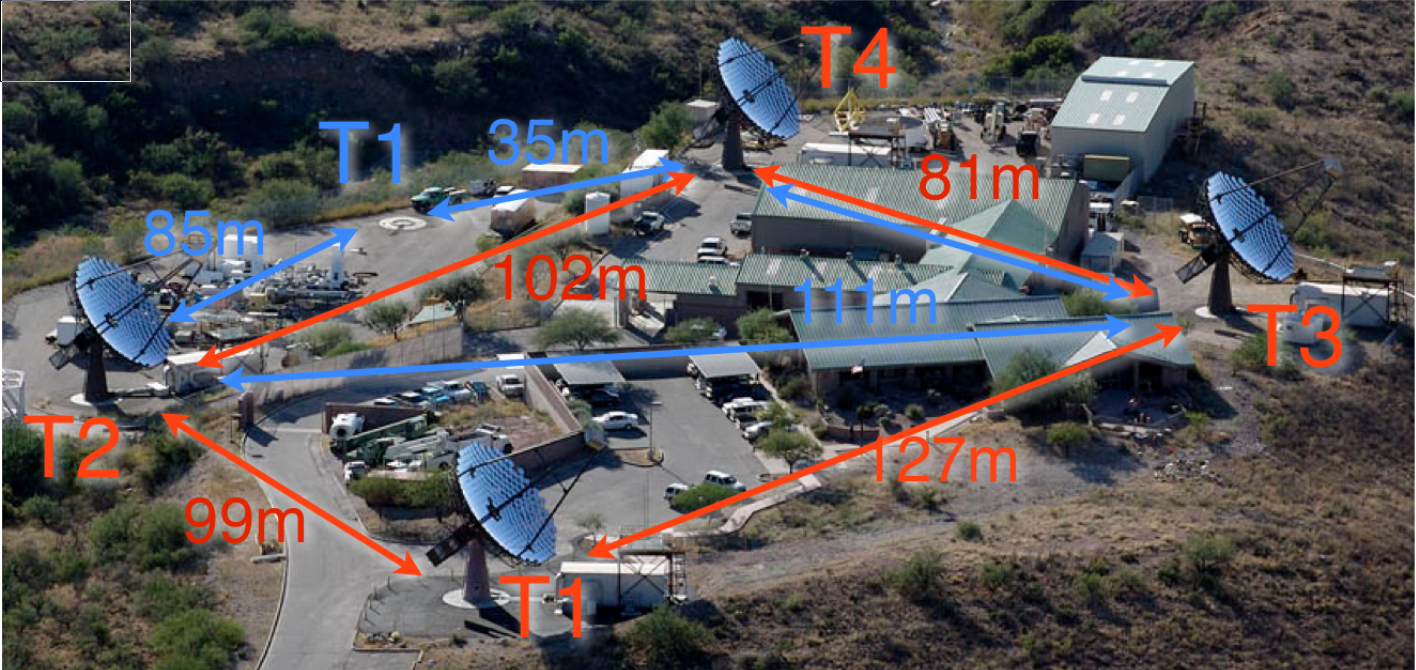
\includegraphics[width=.9\textwidth]{images/veritas_relocation.png}
	\caption{The VERITAS array layout after relocation of the first 
		telescope. The distances between the telescopes are 
		highlighted for the old(blue) and the new(red) array.
		In the old setup the telescopes T1, T2 and T4 were too closely
		located, making their measurements redundant.
	 	The image is taken from an official paper, that investigates
		the improved performance gained by relocating the telescope \cite{2009arXiv0912.3841P}.}
	\label{fig:veritas_relocation}
\end{figure}

Like MAGIC, VERITAS makes use of the DISP-method, especially at large zenith angles 
\cite{2015ICRC...34..771P}.

\subsection{High Energy Stereoscopic System (HESS)}

The HESS experiment consists of five telescopes and 
is - in contrast to MAGIC and VERITAS - operating in the southern 
Hemisphere, in Namibia.

A similar distinction in phase I and phase II as with MAGIC can be taken with 
HESS phase I consisting of four \SI{13}{\meter} diameter telescopes,
arranged at the edge of a square of \SI{120}{\meter} long sides \cite{HINTON2004331}.
These operated from 2004 to 2012 when the experiment went into phase II.

Phase II brought the larger, fifth telescope with the aim to lower the energy threshold
further. This $\SI{24}{\meter} \times \SI{32}{\meter}$-mirror telescope 
was placed in the middle of the other telescopes.
HESS operates at a similar energy range as MAGIC, stating a lower threshold as low as 
\SI{20}{\giga\electronvolt} \cite{vincent2005hess}.


\section{Next to come: The Cherenkov Telescope Array (CTA)}
\label{sec:cta}

The Cherenkov Telescope Array aims to be a next generation IACT experiment.
With two sites of operation, one for each hemisphere, and a number of different 
telescopes proposed, CTA is going to expand on the findings of the third 
generation experiments.

Like HESS in phase II, the CTA arrays are going to consist of different sized telescopes, namely
the Large Sized Telescope (LST, \SI{23}{\meter}), 
the Medium Sized Telescope (MST, \SI{12}{\meter}) 
and the Small Sized Telescope (SST, \SI{4.3}{\meter}).

Extensive Monte Carlo simulations have been performed to find optimal array arrangements
\cite{BERNLOHR2013171}.

The currently planned layouts at LaPalma and in Chile are shown in 
\ref{fig:cta_layout}.
The expected sensitivity compared against other currently operating
experiments is shown in figure \ref{fig:cta_performance}.

\begin{figure}[H]
	\center
	\captionsetup{width=0.9\linewidth}
	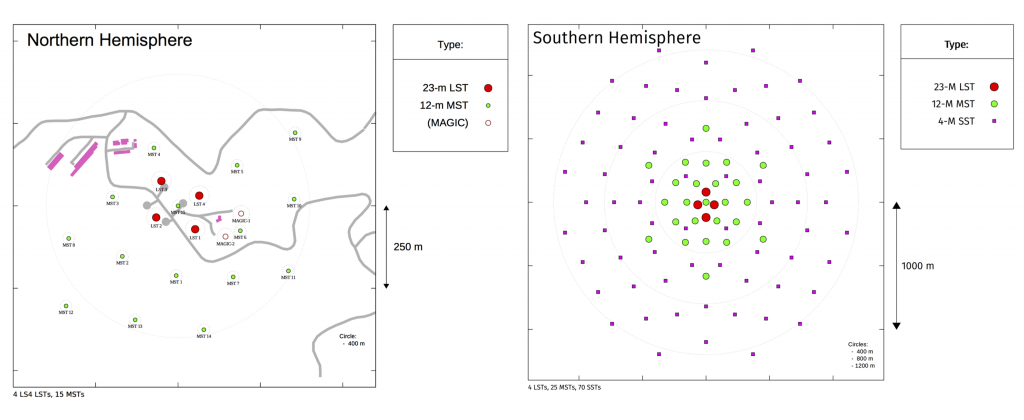
\includegraphics[width=0.9\textwidth]{images/cta_layout.png}
	\caption{
	Left: The array on the northern hemisphere. It will be build at LaPalma
	and feature only LSTs and MSTs.
	Right: The array at the southern hemisphere.
	It will consist of more telescopes and thus 
	work at a bigger energy range.
	The image is taken from the CTA-website \cite{cta_web}.}
	\label{fig:cta_layout}
\end{figure}

\begin{figure}[H]
	\center
	\captionsetup{width=0.9\linewidth}
	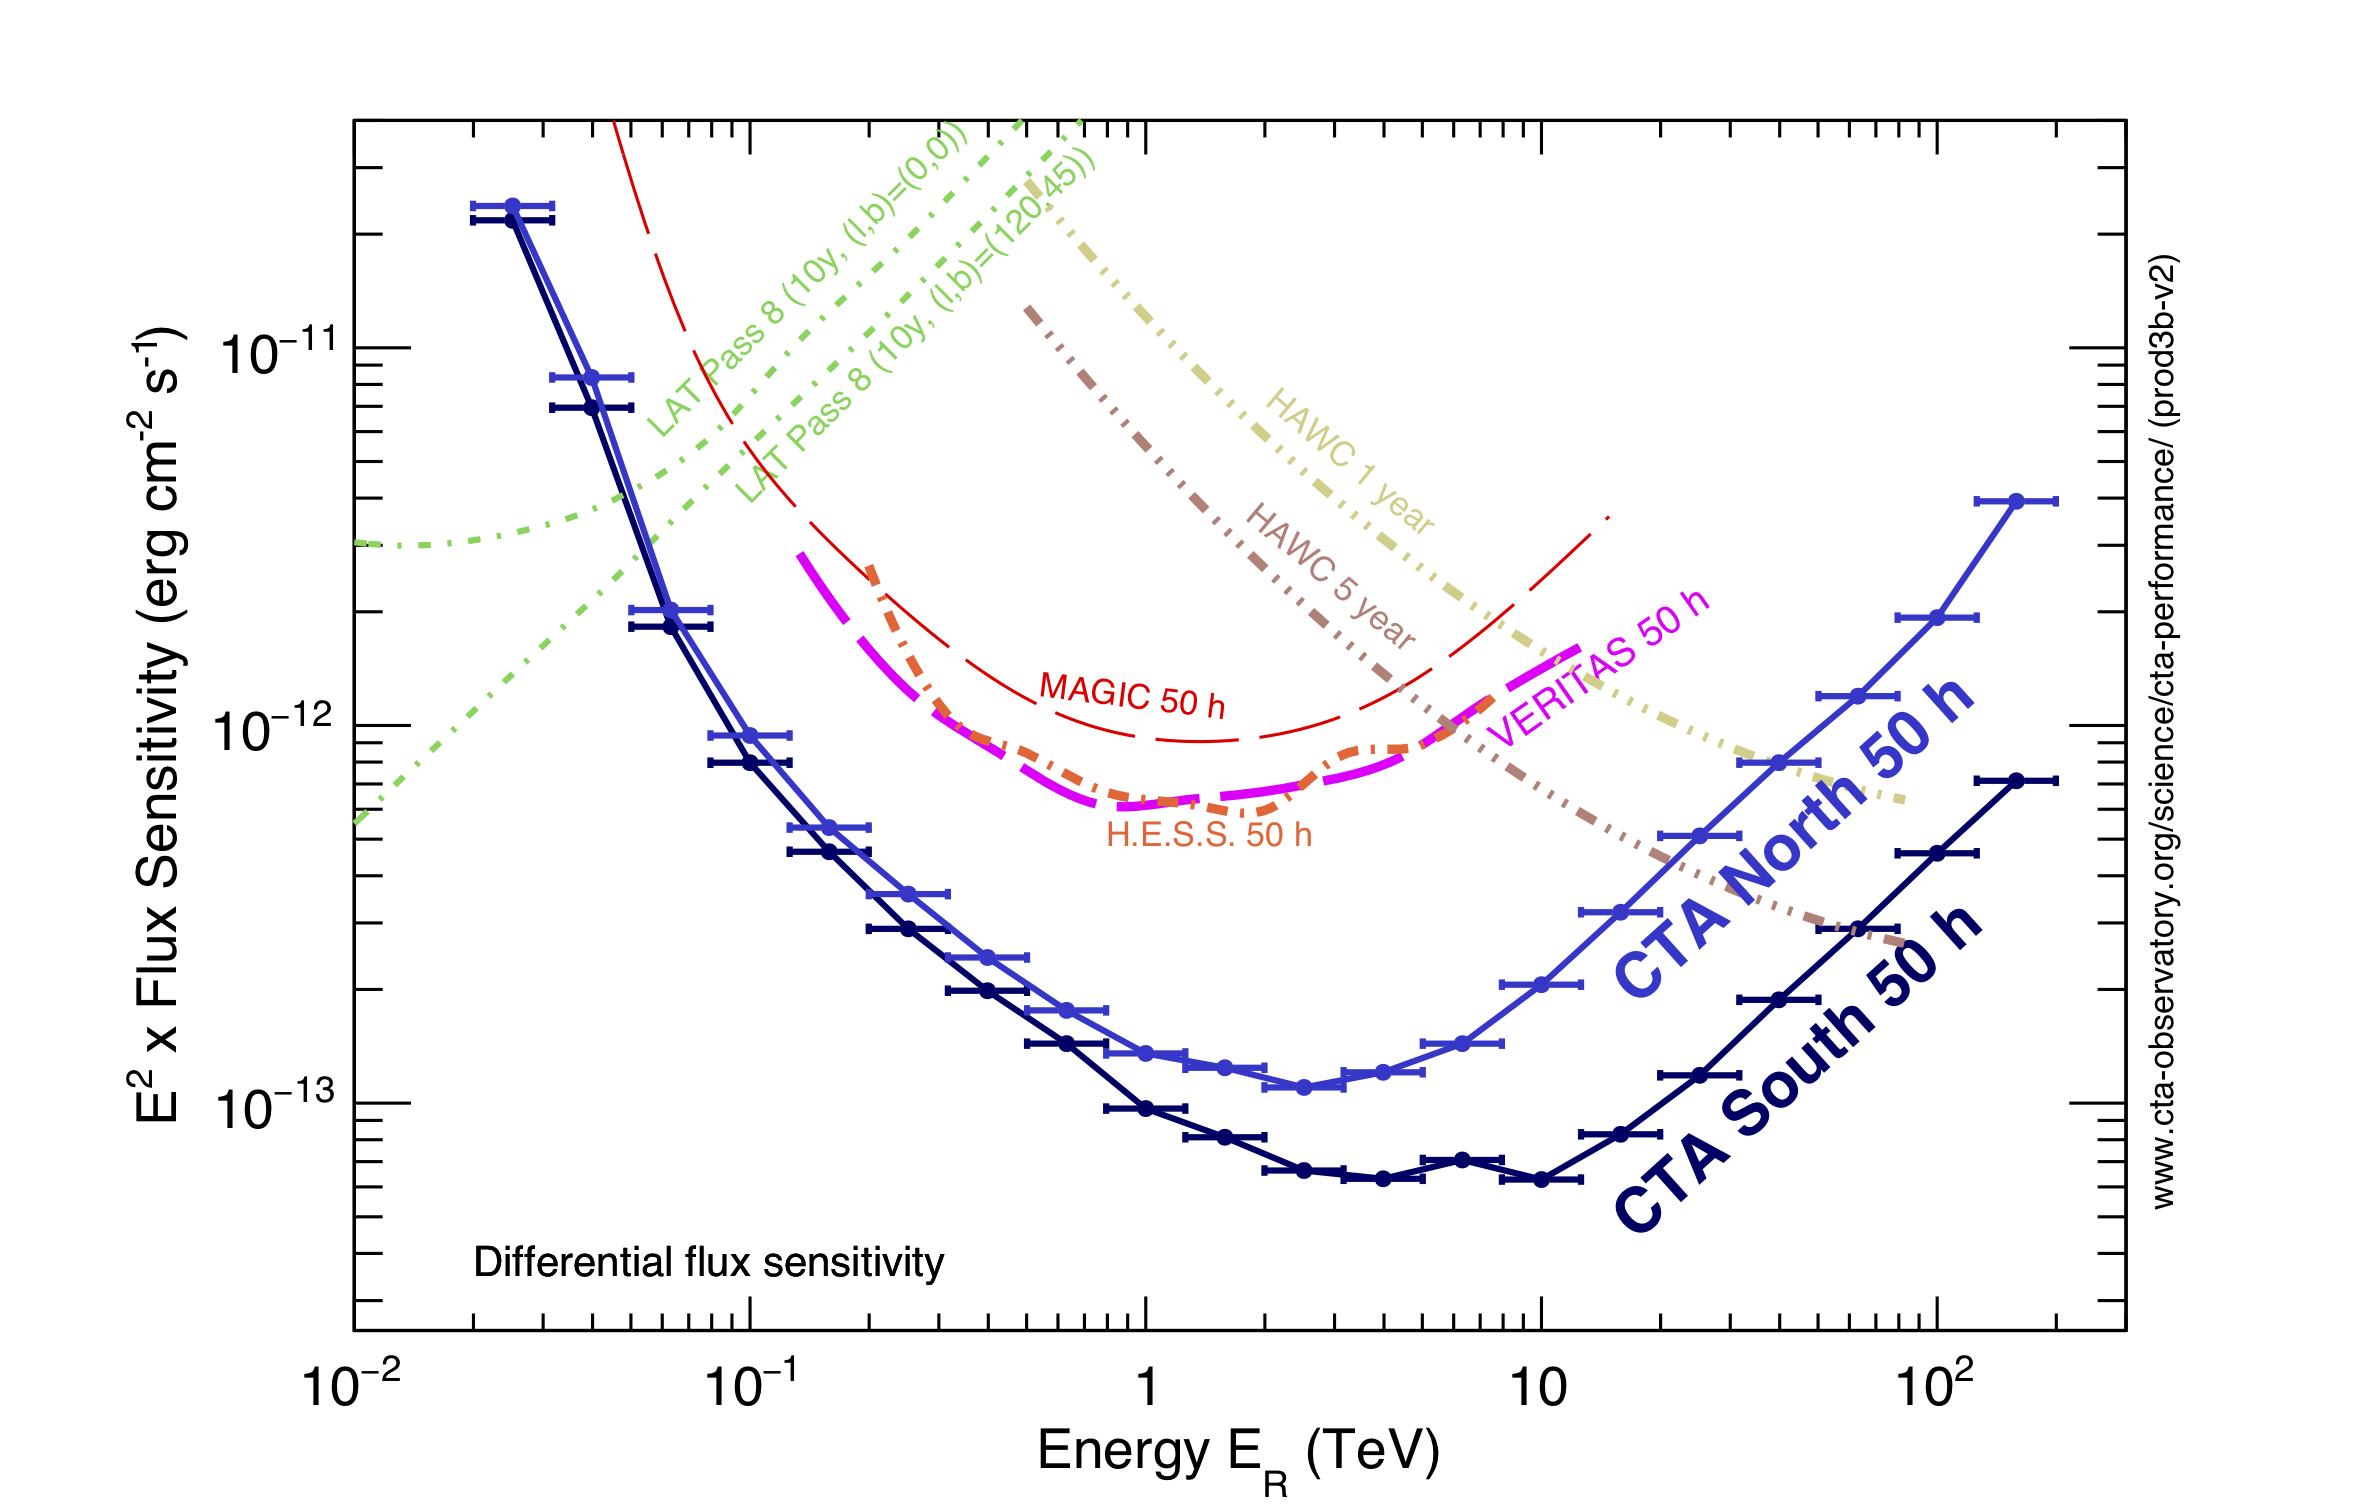
\includegraphics[width=0.9\textwidth]{images/cta_performance.png}
	\caption{A rough comparison of the expected differential sensitivity of CTA compared against
	other experiments. The differential sensitivity is defined as the
	minimum required flux to detect a point source with 5$\sigma$.
	The image is taken from the CTA-website \cite{cta_web}.}
	\label{fig:cta_performance}
\end{figure}

%\newpage
\subsection{LST}
\label{sec:lst}
The Large-Sized Telescope is going to be biggest telescope of CTA
with a mirror diameter of \SI{23}{\meter}.
It will provide the best sensitivity in the energy range from 
\SI{20}{\giga\electronvolt} to \SI{150}{\giga\electronvolt} with a field of view of \SI{4.3}{\degree}.
The camera of the LST, the LSTCamera, has \num{1855} channels 
with \num{265} photomultiplier tubes \cite{cta_web}.

The readout electronic is based on the Domino Ring Sampler 
Version 4 chip, which is also used by the MAGIC experiment
\cite{Kubo:2013pwa}. 

Since the LST is looking for the lowest energy $\gamma$-rays, it needs
very large mirror areas. At the same, time the effective detector area does 
not need to be as high as for higher energy events.
For this reason only 4 telescopes are planned per array.

The first LST has been inaugurated at the 10 October 2018 in La Palma \cite{lst_debut}.
It is foreseen to be the first telescope to be operated by the CTA Observatory.
Until the it has to undergo a critical design review to make sure the performance 
complies with the requirements and expectations.

\begin{figure}
		\centering
		\captionsetup{width=0.9\linewidth}
		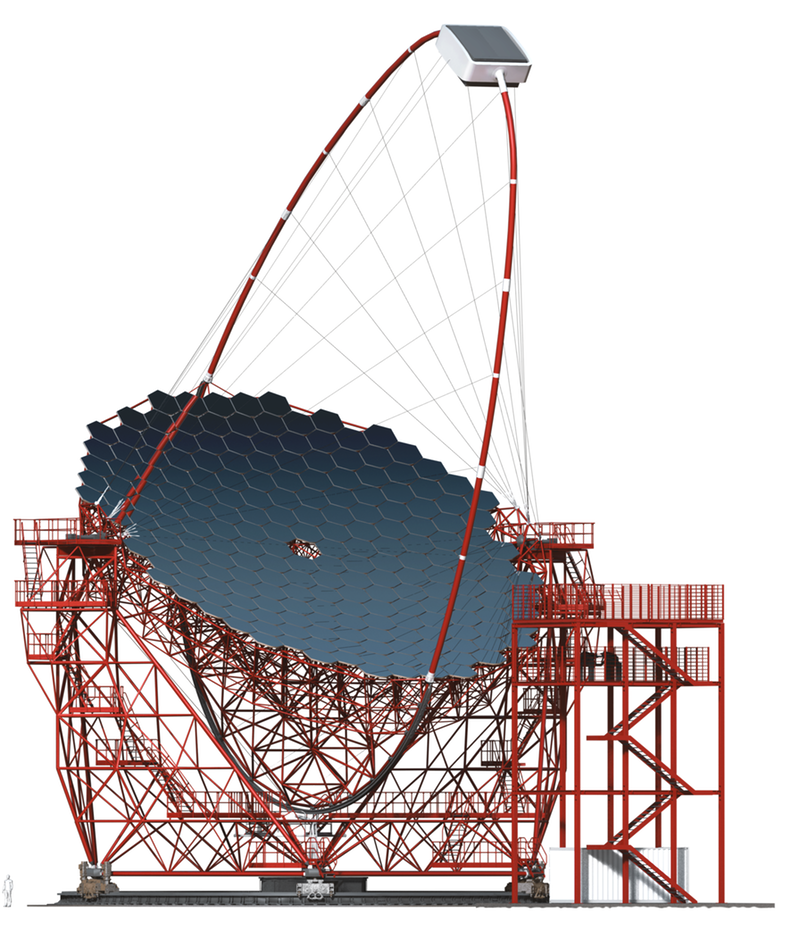
\includegraphics[width=.5\textwidth]{images/LST.png}
		\caption{
			An illustration of the Large Sized Telescope (LST) with its
			\SI{23}{\meter} diameter parabolic mirror.
			In the lower left corner a human is included for scale.
			The image can be found at the official CTA-website \cite{cta_web}.}
		\label{fig:lst}
\end{figure}

%\newpage
\subsection{MST}

\begin{wrapfigure}{R}{0.5\textwidth}
	\centering
	\captionsetup{width=0.9\linewidth}
	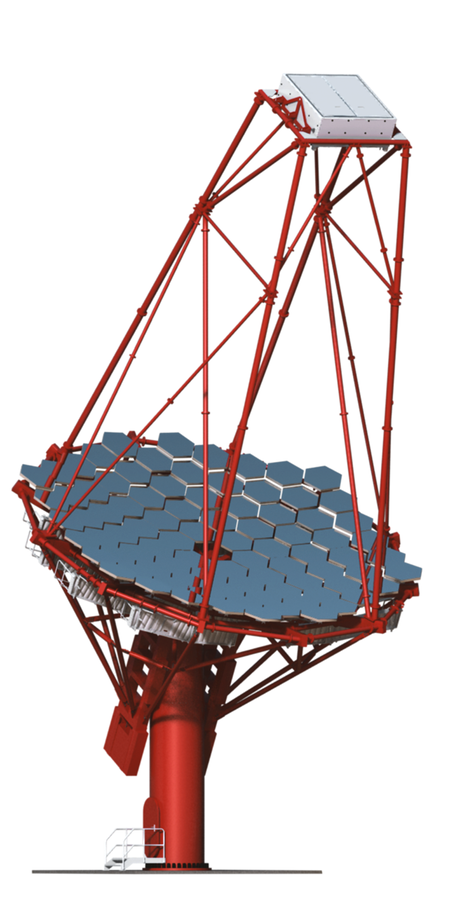
\includegraphics[width=.4\textwidth]{images/MST-1.png}
	\caption{An illustration of the Mediium Sized Telescope (MST) with its
	\SI{11.5}{\meter} diameter mirror.
	The mirror design is based on the Davies-Cotton design.
	The image can be found at the official CTA-website \cite{cta_web}.}
	\label{fig:mst}
\end{wrapfigure}

The Medium-Sized Telescopes (MST) are primarily going to look at the 
energy range from \SI{150}{\giga\electronvolt} to \SI{5}{\tera\electronvolt}.
A total of 15 telescopes on the north site and 25 telescopes at the south site 
are going to be the backbones of CTA.

Two camera designs are being tested for the MST:
The 1764 pixel FlashCam and the 1855 pixel NectarCam \cite{cta_web}.
The flashcam combines twelve PMTs to one module and features a completely
digital readout system.
The nectarcam contains an anlogue readout chip with a high-gain and a low-gain
channel. 7 PMTs are comined to one module \cite{doi:10.1063/1.4969023}.

A prototype for the MST is standing in Berlin .
Besides the camera and readout electronics it is a fully operational telescope
to validate the component design and assembly processes.
% \\
% \\
% \\
% \\
% \\
% \\
% \\
% \\
% \\
% \\

%\newpage
\subsection{SST}

The Small-Sized Telescopes (SST) will provide the sensitivity for CTA at the 
highest energies upwards from \SI{5}{\tera\electronvolt}.
An upper limit for the sensitivity is expected to be around \SI{300}{\tera\electronvolt}.

The design for the SST includes two mirrors, a \SI{4.3}{\meter} and a \SI{1.8}{\meter}
mirror, before the light hits the camera.

In contrast to the LST and MST, the SST's camera includes silicon photo-multipliers
and a total of 2048 pixels. With this the SST is going to cover a field of view 
of \SI{10.5}{\degree}.

The north array is not going to include any SSTs, the 
south array on the other hand will contain a total of 70 telescopes over
several square kilometers \cite{cta_web}.

\begin{figure}
		\centering
		\captionsetup{width=0.9\linewidth}
		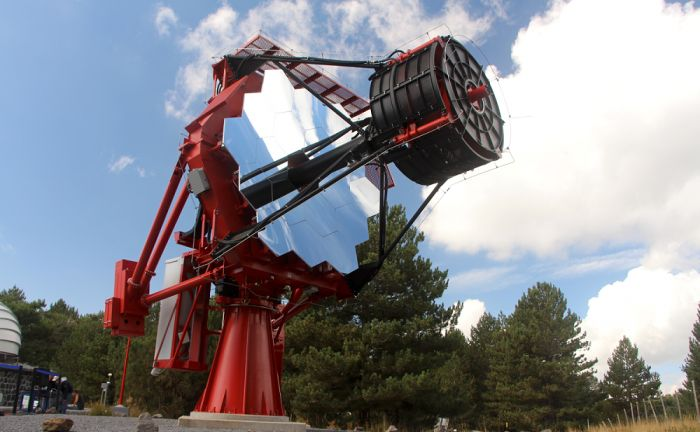
\includegraphics[width=.9\textwidth]{images/sst.jpg}
		\caption{An illustration of the Small Sized Telescope (SST) with its
		two mirrors.
		The dual-mirror Schwarzschild-Couder setup includes mirrors of
		\SI{4.3}{\meter} and \SI{1.8}{\meter} diameter.
		The image can be found at the official CTA-website \cite{cta_web}.}
		\label{fig:sst}
\end{figure}
% \chapter{analysis}\label{analysis}

ToDo:
\begin{enumerate}[nosep]
    \item Datenformat Input, verwendete Daten, Worte zu Simulation, trainingsdaten
    \item Preprocessing - Schritte erklären
    \item Datenformat Output Preprocessing
    \item ...
    \item Anwendung Random Forests mono, disp erklären anhand hillas parameter
    \item Anwendung Stereo (Random forest, stabile Mittelwertverfahren -alle erklären)
    \item Signifikanzkurve
\end{enumerate}

\section{preprocessing}
% configuration in appendix! + algorithmen beim prep

\subsection{Monte Carlo Data}
At the lowest level our observed data consists of uncalibrated waveforms 
in the camera pixels.
prod3b stuff kurz anreißen
wahl des arrays!

\subsection{Reconstruction on telescope level+hillas reconstructor}
% definition datenlevel
- calibration
- cleaning
- hillas parameters 
- telescope level
- tabellen der features bei runs/arrays/telescopes

To be able to apply high-level analysis methods, the initial data 
needs to be reduced and preprocessed substantially.

To specify a specific event, we will identificate an event based on 
three layers:
\begin{enumerate}
    \item{Run-Id: This gives us non-event-specific information about the monte carlo run, e.g.
    spectral\_index, particle injection height, ...}
    \item{Array-event-id: Any shower that triggered the array is considered to be an array event.
    Array-level features consist of general event information (e.g. number of triggered telescopes, average internsity)
    reconstructed features of the primary particle (energy, source position, ...) and the 
    event specific monte carlo information to compare these features against.}
    \item{Telescope-event-id: This specifies how a specific telescope has seen the shower and
    contains information about the telescope itself (e.g.focal length). Telescope-level features 
    describe the camera image, amongst other things via the hillas-parameters(cite stuff)}
\end{enumerate}


In the following we will 
distinguish between "array-events" and "telescope-events" when describing the reconstruction methods.

Processing of the Simtel-files is done with the aforementioned ctapipe, starting with 
the calibration of the (array) event. This performs an integration of the waveforms in 
each pixel of the camera of a triggered telescope. Inside ctapipe the initial data is referred to as R1
and the reuslting data as dl1. The resulting images get cleaned with a tailcuts approach before they are
used to calculate image features, such as the hillas parameters.

Hier part über hillas params mit den bildern! erklären wieso und so
\begin{figure}
    \begin{subfigure}{0.3\textwidth}
        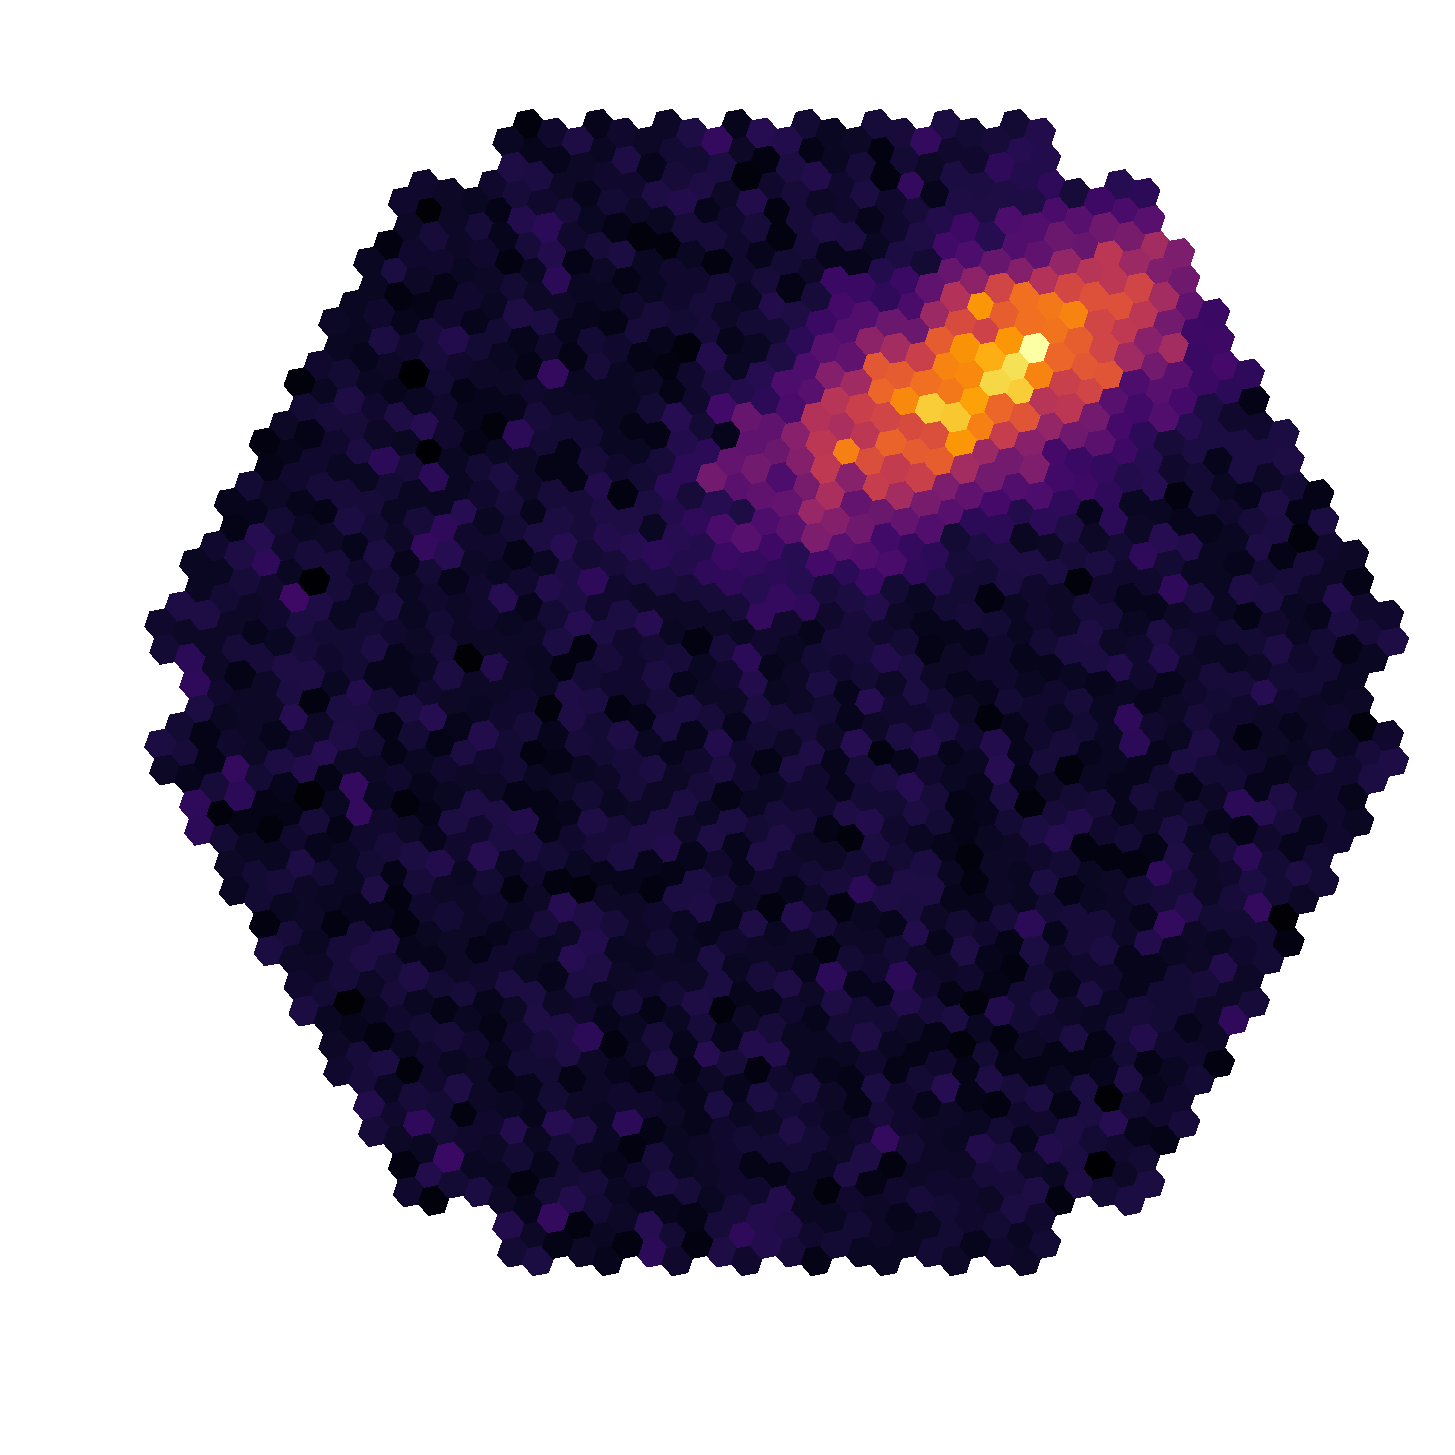
\includegraphics[width=0.9\linewidth]{Plots/hillas_raw.pdf} 
        %\caption{Caption1}
        \label{fig:shower_image_raw}
    \end{subfigure}
    \begin{subfigure}{0.3\textwidth}
        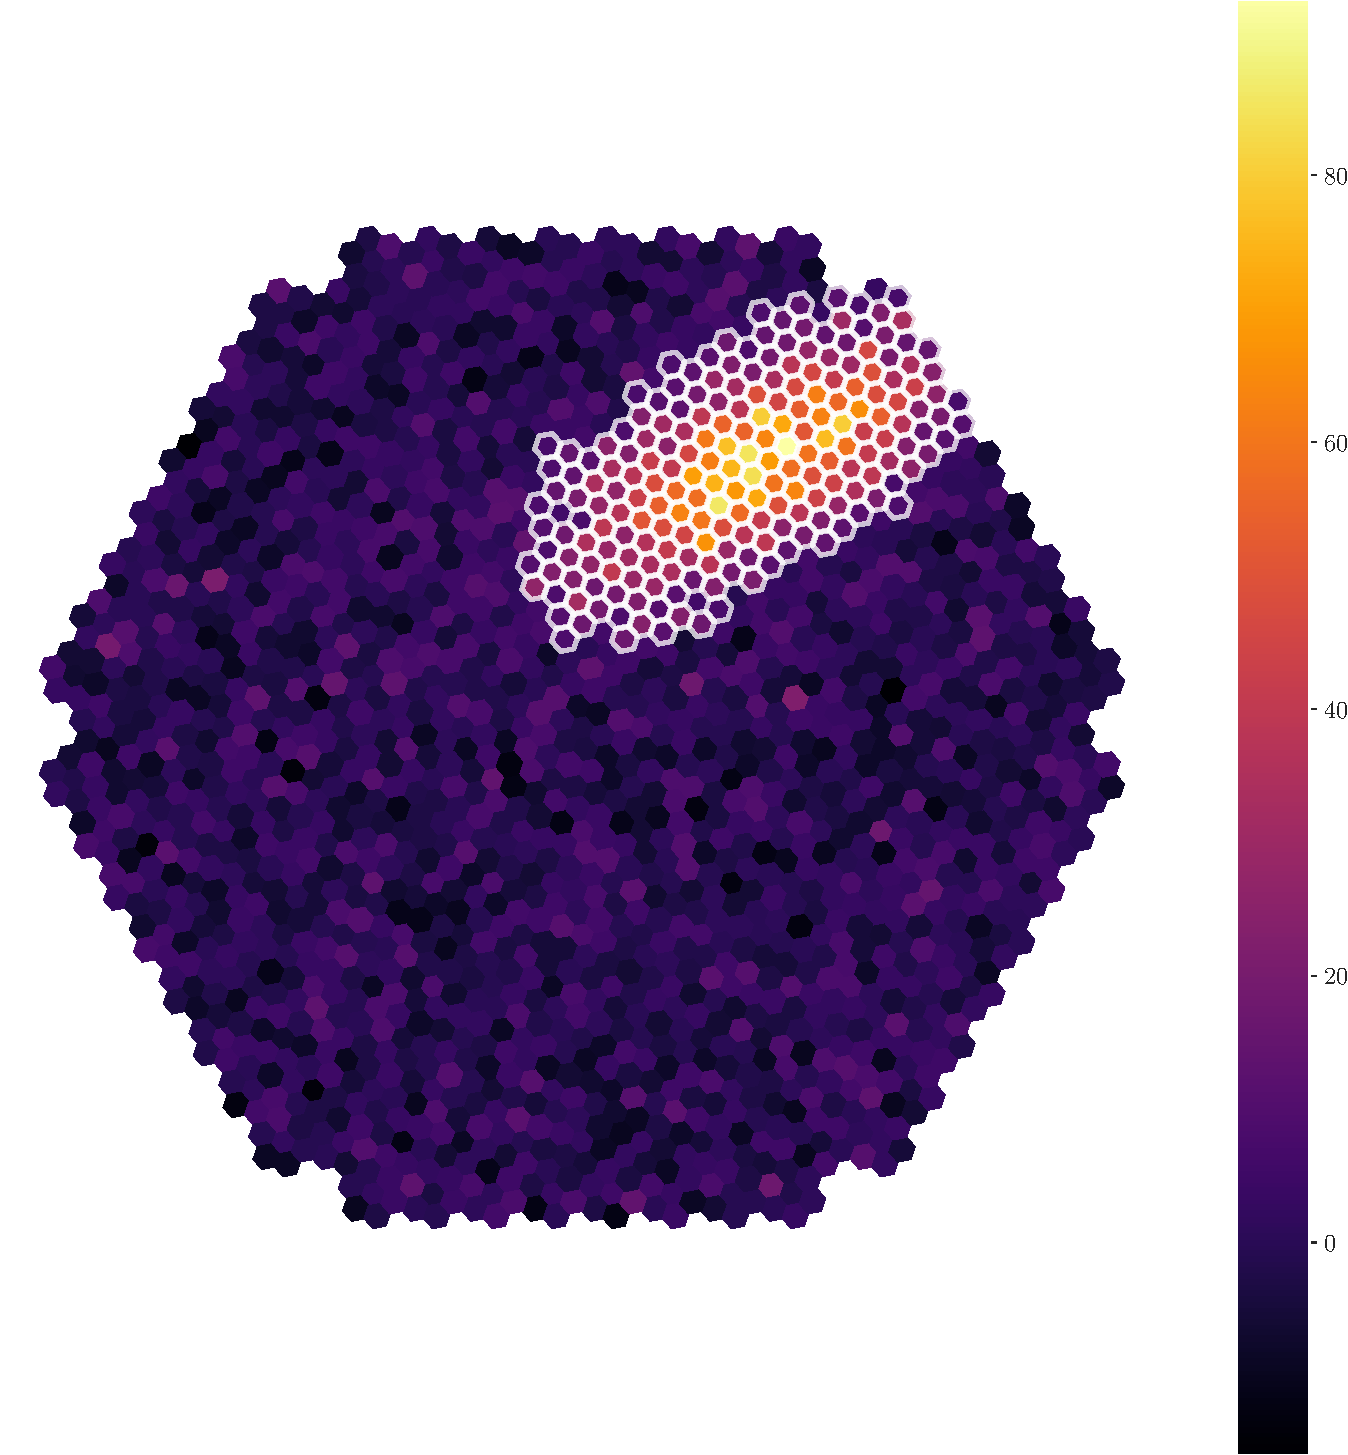
\includegraphics[width=0.9\linewidth]{Plots/hillas_cleaned.pdf}
        %\caption{Caption 2}
        \label{fig:shower_image_cleaned}
    \end{subfigure}
    \begin{subfigure}{0.3\textwidth}
        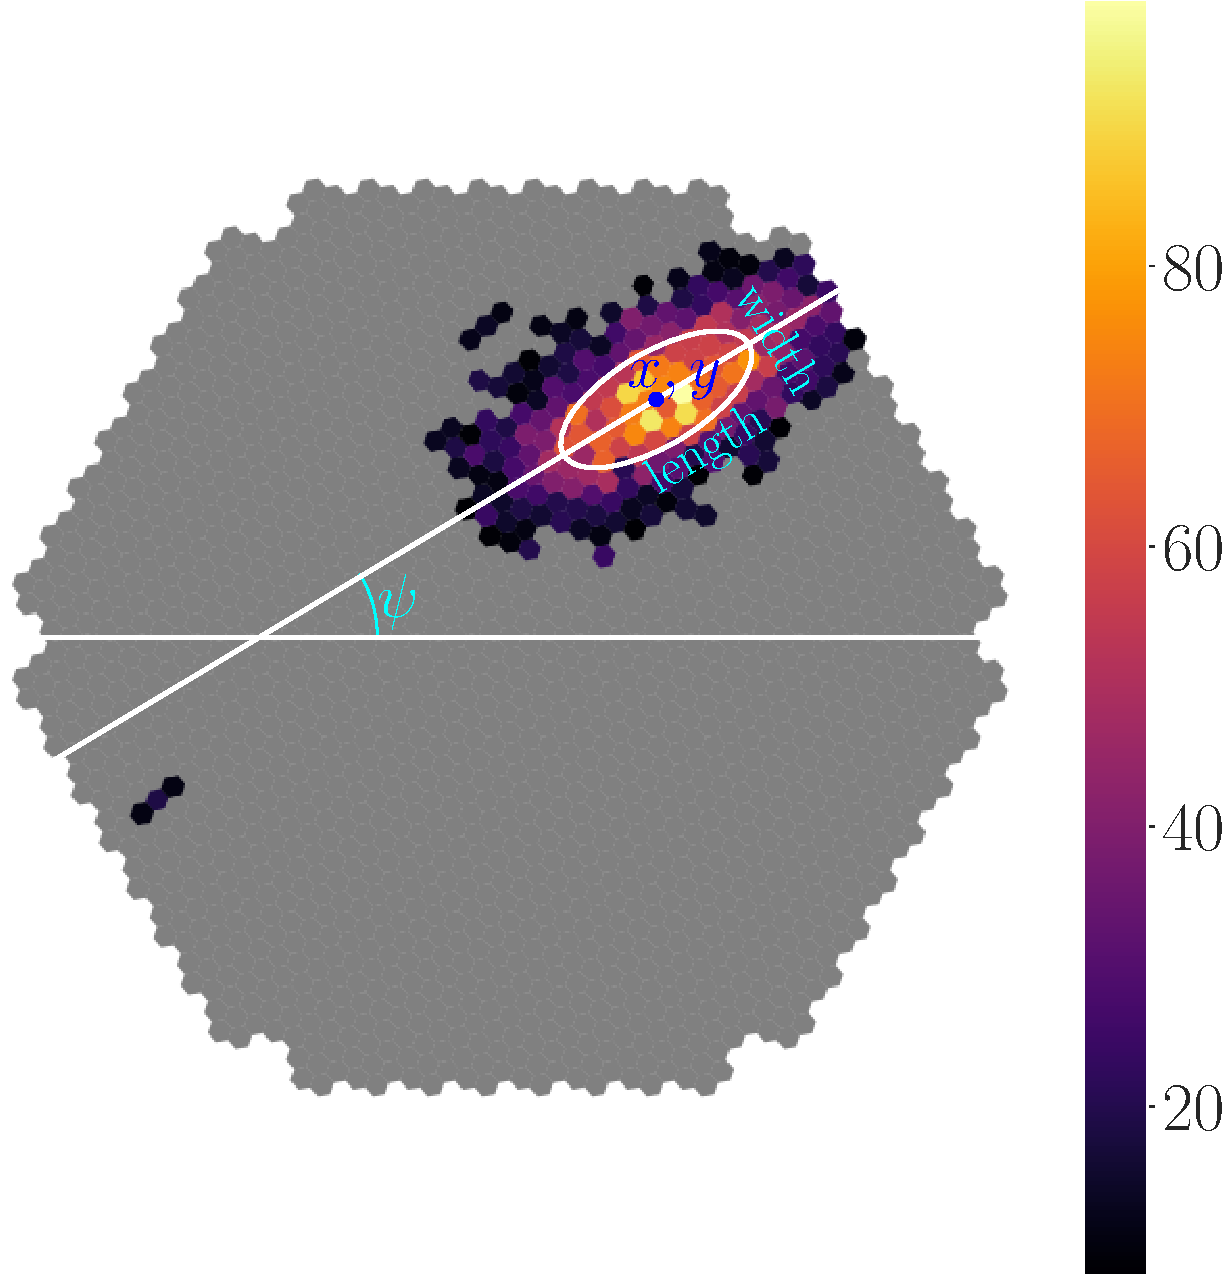
\includegraphics[width=0.9\linewidth]{Plots/hillas_cleaned_params.pdf} 
        %\caption{Caption1}
        \label{fig:hillas_parameters_only}
    \end{subfigure}
    \caption{Illustration of a simulated gamma shower captured with the LST-telescope.
        The left figure shows the image after applied waveform-extraction but before
        the cleaning step. The right figure shows the image after the cleaning has been applied
        and non-selected pixels have been discarded.}
    \label{fig:shower_image}
\end{figure}

In addition to the original hillas parameters, the concentration, number of islands and timing parameters
get calculated.
Concentration refers to the intensity captured in the brightest pixel or the cog relative to 
the total intensity in the image.
An island is considered a connected cluster of pixels. In an ideal gamma shower image, only one island
is expected, although this is highly dependend on the applied cleaning.
Timing parameters are the second momenta of the distribution of the relative peak arrival times
in each pixel, which can be derived form the waveforms.

All these features get used in the machine learning algorithms at later stages.

\subsection{Hillas reconstructor}  % we dont seperate between 0 and 1 right?
After the image processing of each associated telescope image has been finished,
the predictions of our "baseline" source position estimator get calculated.
This algorithm is referred to as HillasReconstructor inside ctapipe, because 
it works based on the hillas parametrisations of the images.
For each triggered telescope, a 2D-plane is drawn based on the main shower 
axis and the telescope orientation. These planes intersect and 
the weighted average of all intersections gives the 
direction of the shower origin (cite code or paper).

%% input ausgelagerten hillas tikz kram

Since this method inherently requires a stereoscopic experiment
and multiple triggered telescopes, it will not work for a single telescope.
From earlier studies (kram zitieren, zb kai), it is expected
that this method works best with an event multiplicity 
(number of triggered telescopes) \geq 3 with higher multiplicity
leading to better results.

\section{Machine Learning, dl3?}
High level analysis of the preprocessed data is based on the use of
the aict-tools \cite{aict-tools} package which itself is based on
sklearn \cite{sklearn_api} for the machine learning algorithms.
The algorithm of choice is the Random Forest algorithm
as it is well suited for the use with tabluar data and tends to rarely overfit
(citation needed).
Seperate models are trained for the tasks of signal/background
separation, signal energy estimation and signal source position
reconstruction.
The aict-tools have originally been developed for the FACT-experiment
(citation needed) which is a single IACT. For this reason
adaptions had to be made to perform a stereoscopic analysis.


\subsection{g/h sep}
For the task of gamma/hadron separation a random forest can be trained
using either only monoscopic information or also using array-level
information from earlier reconstruction steps.
This generally improves the accuracy by a few percent points.
The single telescope predictions can be combined by
simple functions such as the mean or median of the
single predictions to provide a prediction for the complete
array-event.
% features und kram


% \section{energy estimation}
% Energy estimation can be performed in the same way as the gamma/hadron
% separation. For this task there has been earlier work indicating
% the usefulness of a second machine learning model trained
% on the predictions of the first telesope-level model
% \cite{ba-lars}.

% I am thus going to present results based on either calculating the mean
% of the telescope level predictions and using a second random forest
% to improve the array level prediction.

\subsection{source position}
\label{sec:source_position}
Given the source position in the camera frame the source position
on the sky can be calculated with coordinate transformations if
the position, pointing and optical properties of the
telescope are known.
In general the true source position in the camera frame is assumed to be
different from the center of gravity of the shower ellipse
but located somewhere along the main shower axis.
This assumption seems to hold decently well, .... zitat.

The position on the shower axis can be estimated based on 
the hillas parameters and other image features.
This method is known as the DISP-method in the
literature (citation needed). The general idea 
can be seen in figure \ref{fig:disp}.

\begin{figure}
    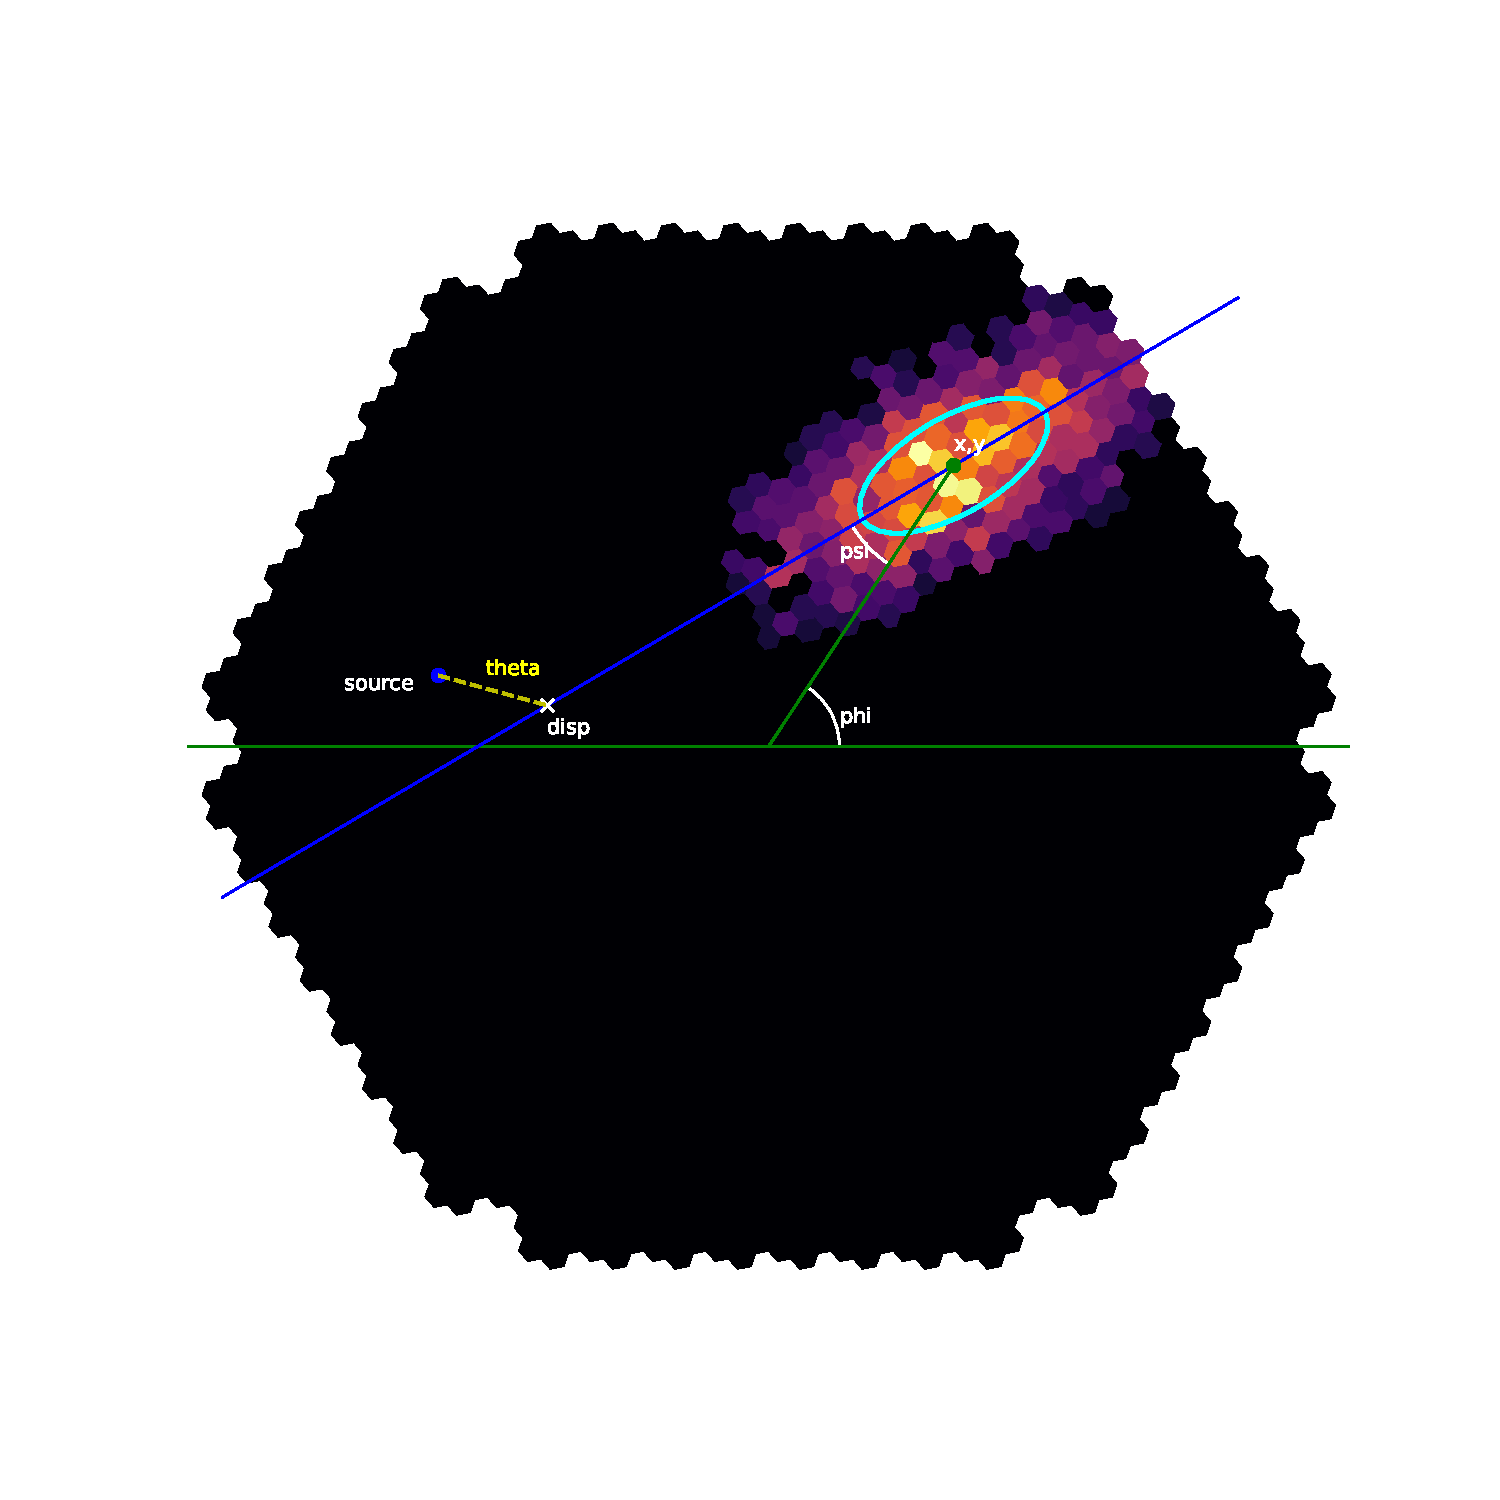
\includegraphics[width=0.9\linewidth]{Plots/hillas_complete.pdf}
    \caption{Illustration of monoscopic source position reconstruction making use of 
        the Hillas-Parameters and the DISP-method as explained in section \ref{sec:source_position}.
        The left figure has the hillas ellipse and parameters drawn onto our previously cleaned sample shower.
        The right figure estimates a source Position in the Camera frame.}
    \label{fig:disp}
\end{figure}

With the DISP-method the estimated distance between the source
position and the center of gravity of the hillas ellipse gets calculated
based on the form of the ellipse, timing information and potentially
more features.
This can be done analitically, via lookup-tables or with machine learning.
At this point the reconstructed source position
is fixed at two points at the main shower axis, see figure \ref{fig:disp_amb}


\begin{figure}
    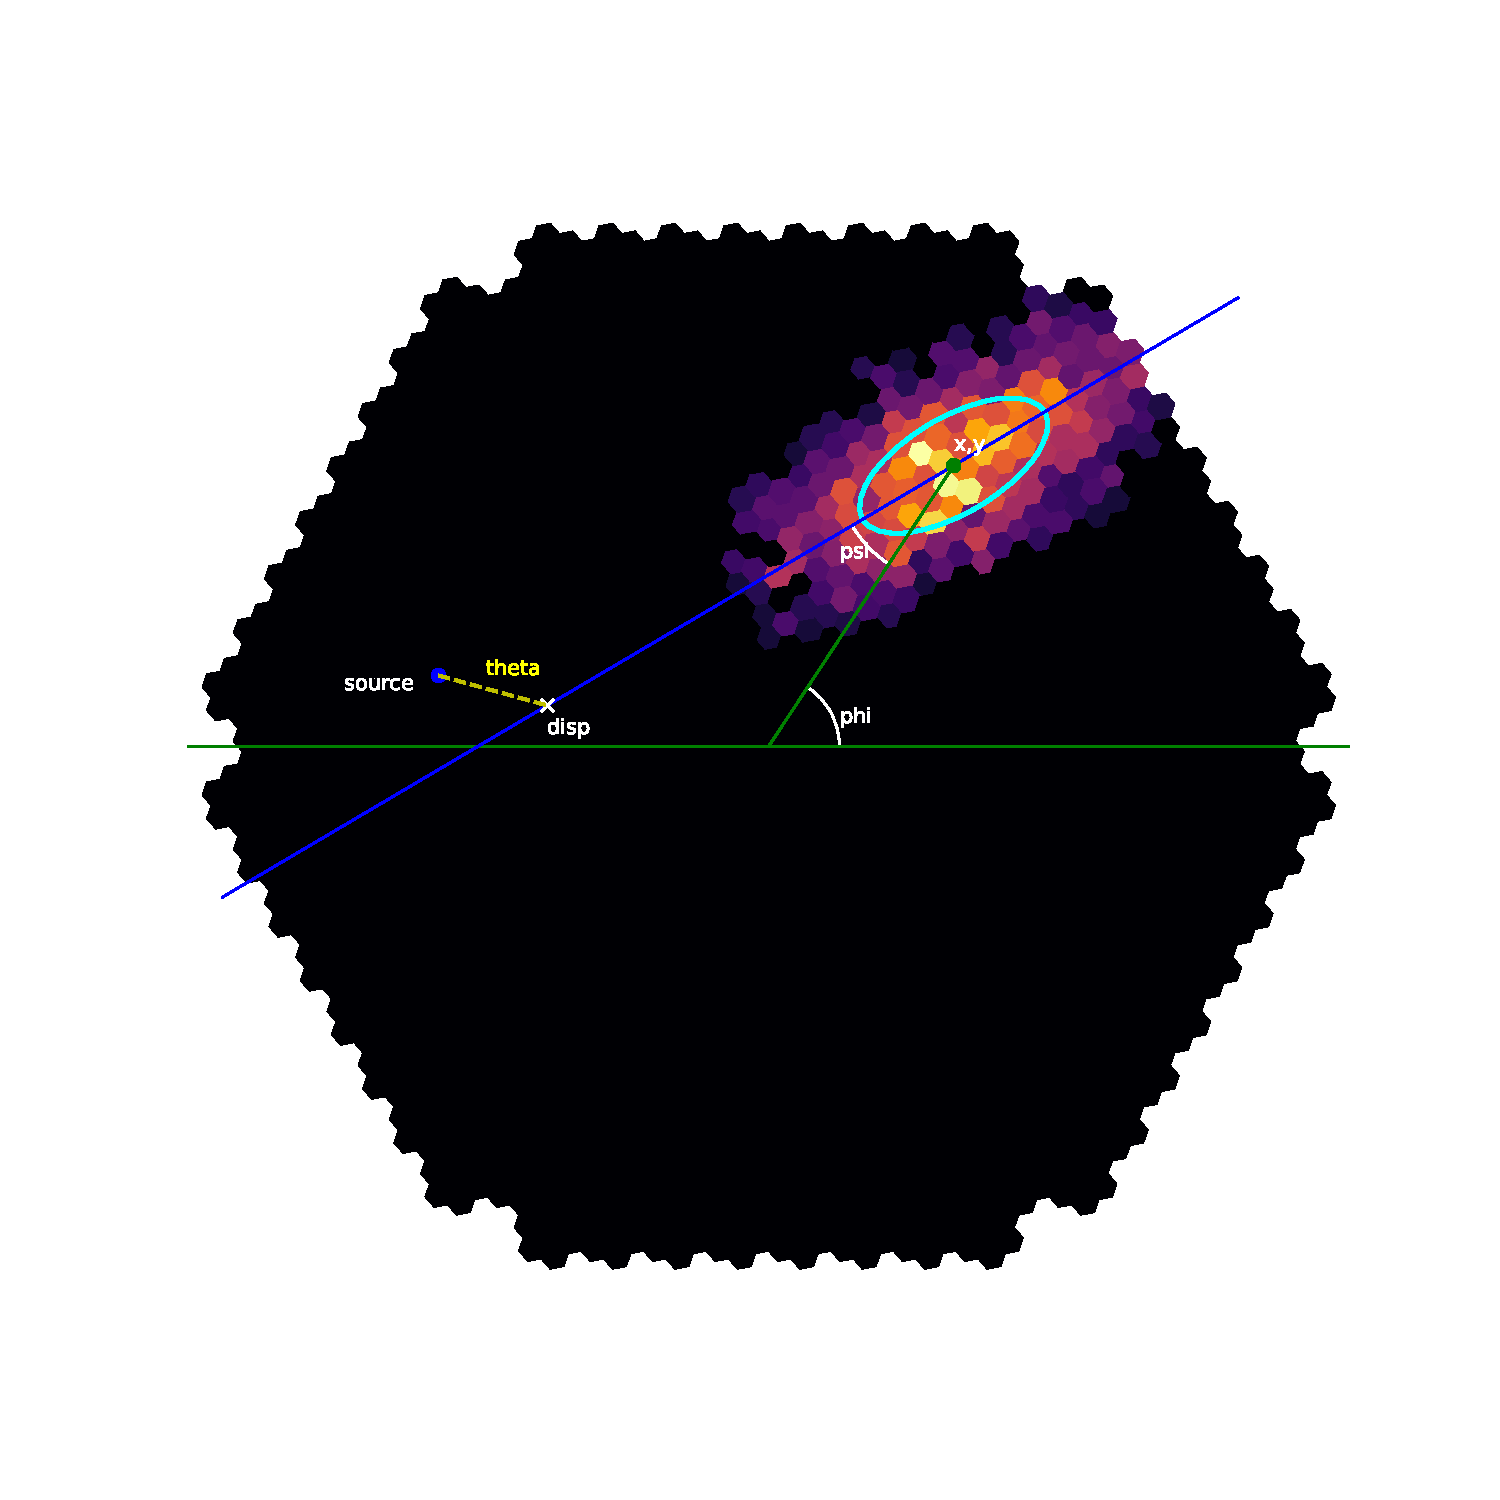
\includegraphics[width=0.9\linewidth]{Plots/hillas_complete.pdf}
    \caption{Wrong pic!}
    \label{fig:disp_amb}
\end{figure}


The remaining task then consists of finding the correct one of these
two points. If there is no stereoscopic information available,
a choice can be made based on the image features again.
In FACT-analyses a second random forest is trained for this
specific purpose, usually yielding an accuracy around 70-80\% (citation).
This is called SIGN-prediction, interpreting the two possible sides
as +-1, allowing for binary classification.
In the case of the MAGIC-telescopes the ambiguity does not
get resolved until the individual results get combined
on the stereo level. The choice of the correct
pair out of the four reconstructed positions can be done either
by calculating the crossing point of both main shower axises
or by calculating the pairwise distances between the positions (citation).


These methods are illustrated in figure \ref{fig:disp_magic}


\begin{figure}
    \begin{subfigure}{0.3\textwidth}
        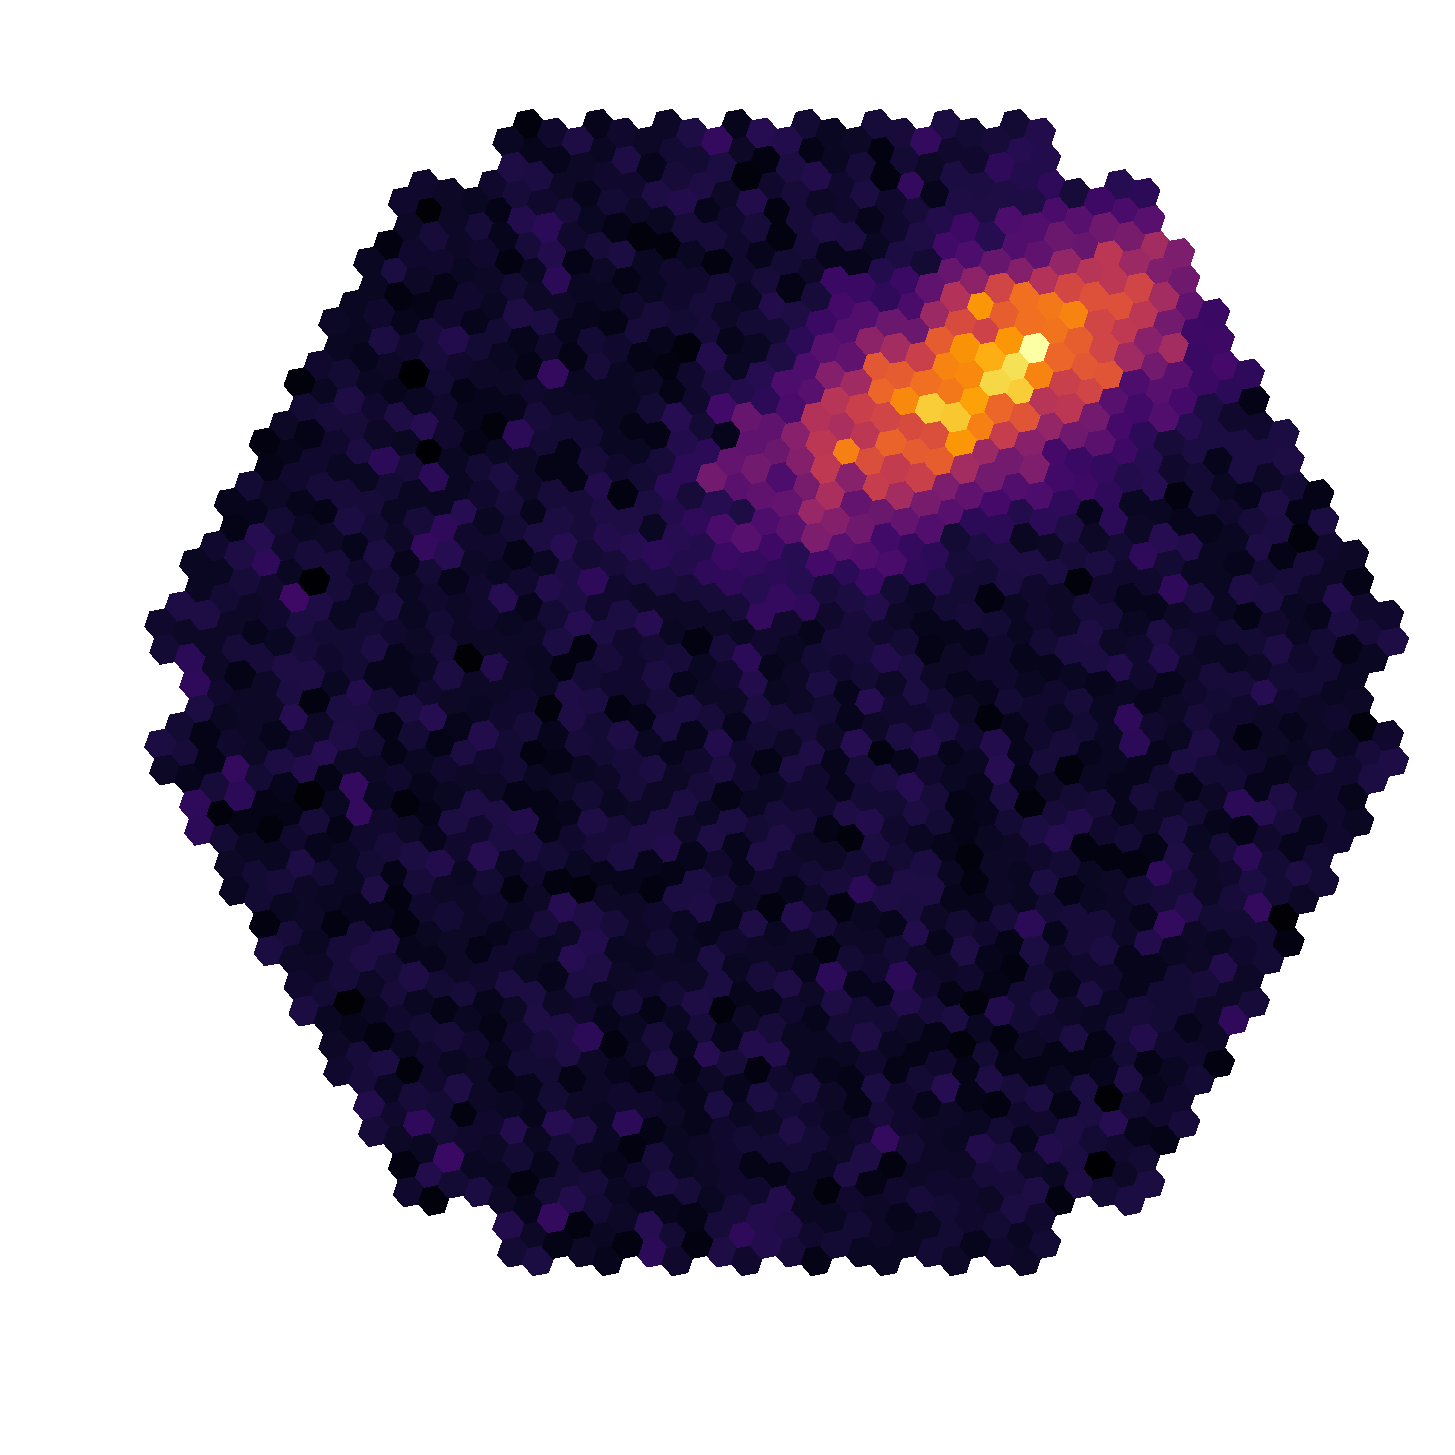
\includegraphics[width=0.9\linewidth]{Plots/hillas_raw.pdf} 
        %\caption{Caption1}
        \label{fig:3}
    \end{subfigure}
    \begin{subfigure}{0.3\textwidth}
        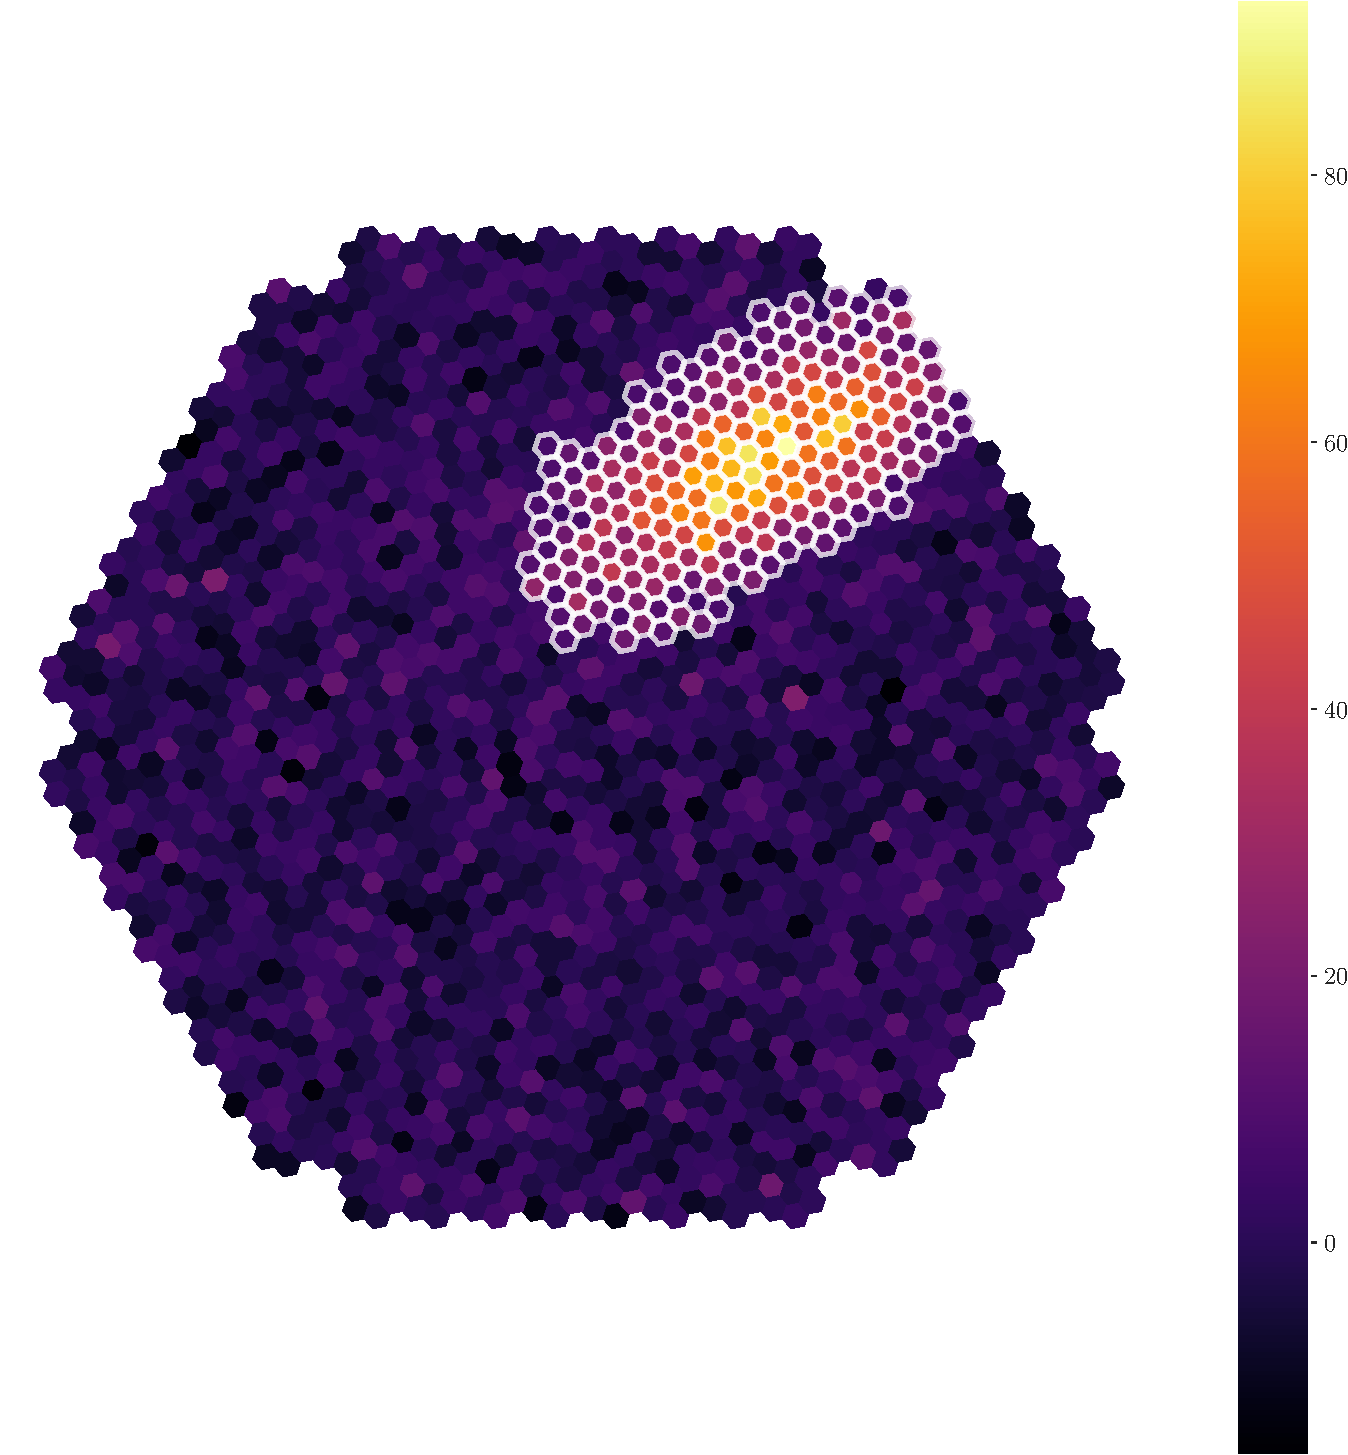
\includegraphics[width=0.9\linewidth]{Plots/hillas_cleaned.pdf}
        %\caption{Caption 2}
        \label{fig:2}
    \end{subfigure}
    \begin{subfigure}{0.3\textwidth}
        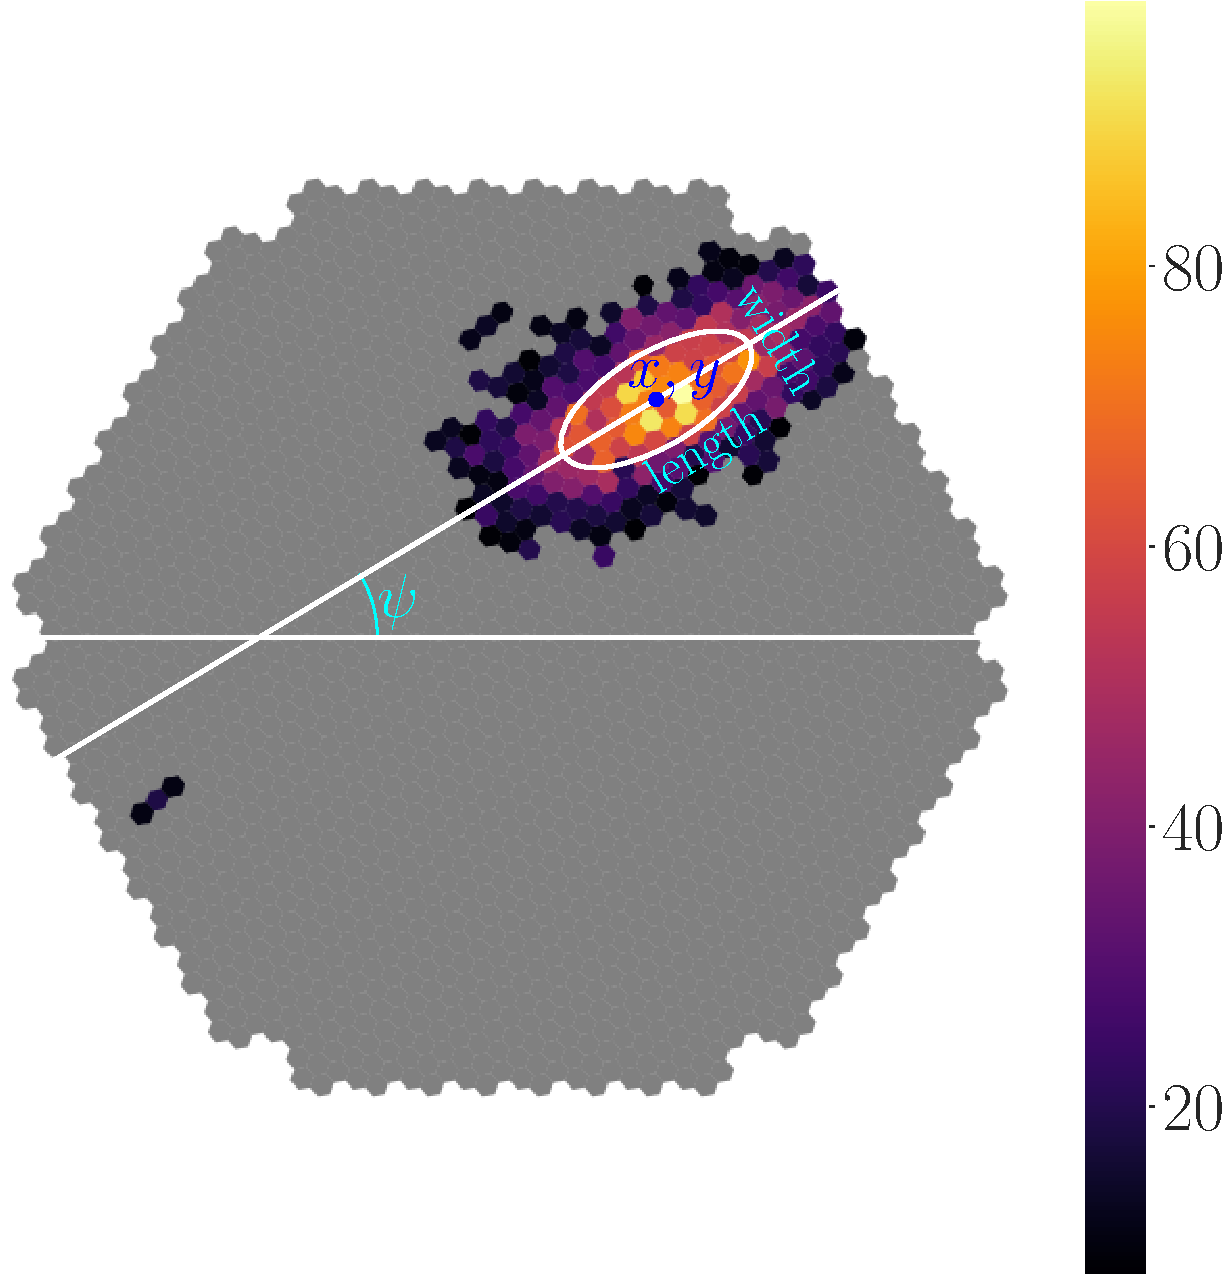
\includegraphics[width=0.9\linewidth]{Plots/hillas_cleaned_params.pdf} 
        %\caption{Caption1}
        \label{fig:1}
    \end{subfigure}
    \caption{wrong pics}
    \label{fig:disp_magic}
\end{figure}





\section{Analysed Data}
\subsection{Corsika Simulation}
\subsection{Training, Testing, mismatches und so, weniger telescope daten bei weniger teleskopen! duh... aber wichtig für statistik.}

% \chapter{results}\label{results}


\section{ghsep}\label{ghsep}

The random forest for the gamma-/hadron-separation gets trained on 
\num{5753708} diffuse gamma events and \num{6035652} diffuse proton events with a 5-fold cross-validation.
We define the class gamma to be of value 1 and protons of value 0.
The random forest predicts a "gammaness" between 0 and 1.
With these parameters, the distribution of the predicted gammaness
is illustrated in figure \ref{fig:gh_sep}.

\begin{figure}
    \centering
    \includegraphics[page=2, width=.8\textwidth]{../analysis/plots/cross_val_sep_perf_plot.pdf}
    \caption{Distribution of the predicted gammaness on the cross-validated training data.
	    The two populations (Proton and Gamma, marked in blue and orange), can be separated 
	    to a certain degree. Over $\approx \num{0.5}$ the preidctions for protons decrease rapidly.
        A perfect prediction (AUC=1) would show no overlap between the distributions.}
    \label{fig:gh_sep}
\end{figure}

The ROC-curve is shown in figure \ref{fig:gh_roc}, with the model achieving an AUC of 
\num{0.835}.


\begin{figure}
    \centering
    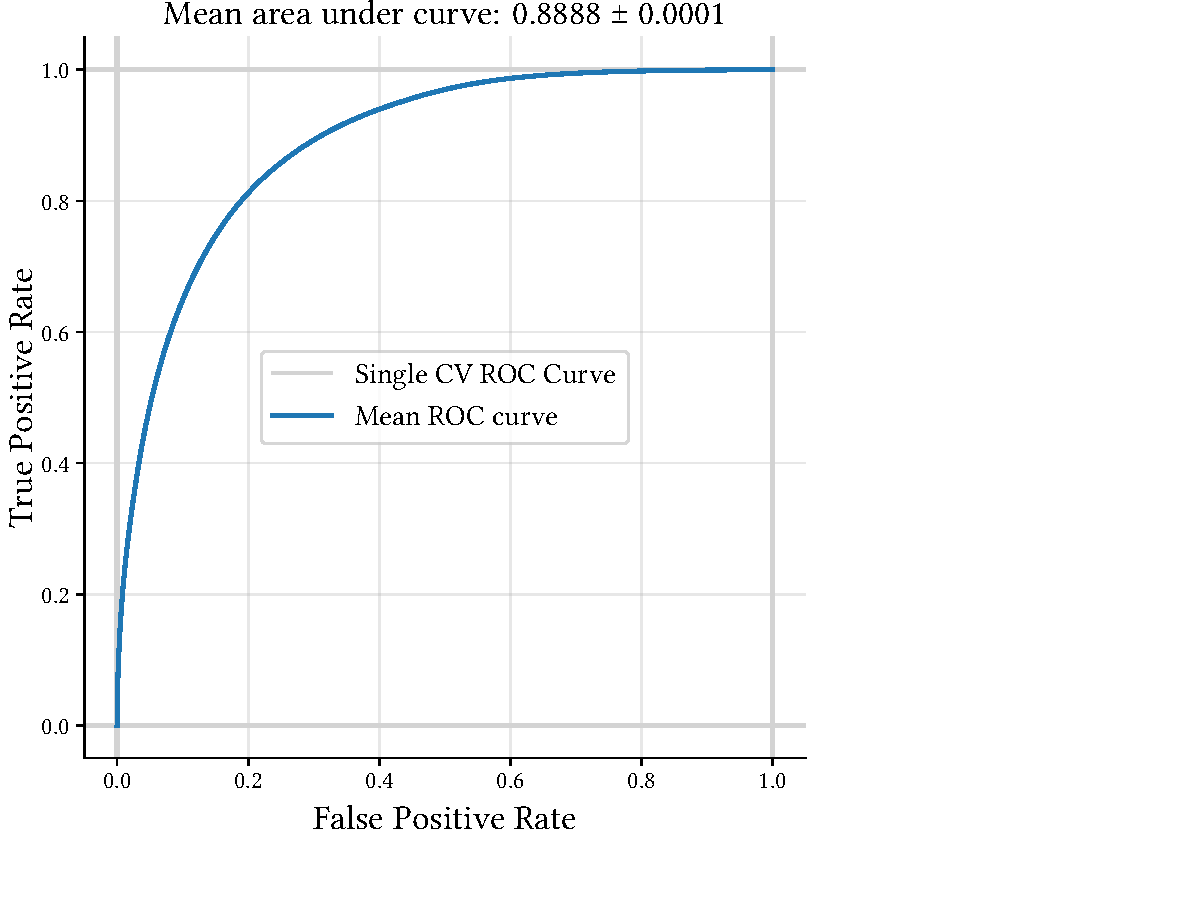
\includegraphics[page=1, width=.8\textwidth]{../analysis/plots/cross_val_sep_perf_plot.pdf}
    \caption{ROC-curve for the gamma/hadron separation on the cross validated training set 
    consisting of \num{6035652} proton events and \num{5753708} diffuse gamma events in total.
    The five ROC-curves from the individual cross validation steps show almost no deviation.}
    \label{fig:gh_roc}
\end{figure}


The feature importance, as calculated via sklearn, is shown in figure \ref{fig:gh_features}.
\begin{figure}
    \centering
    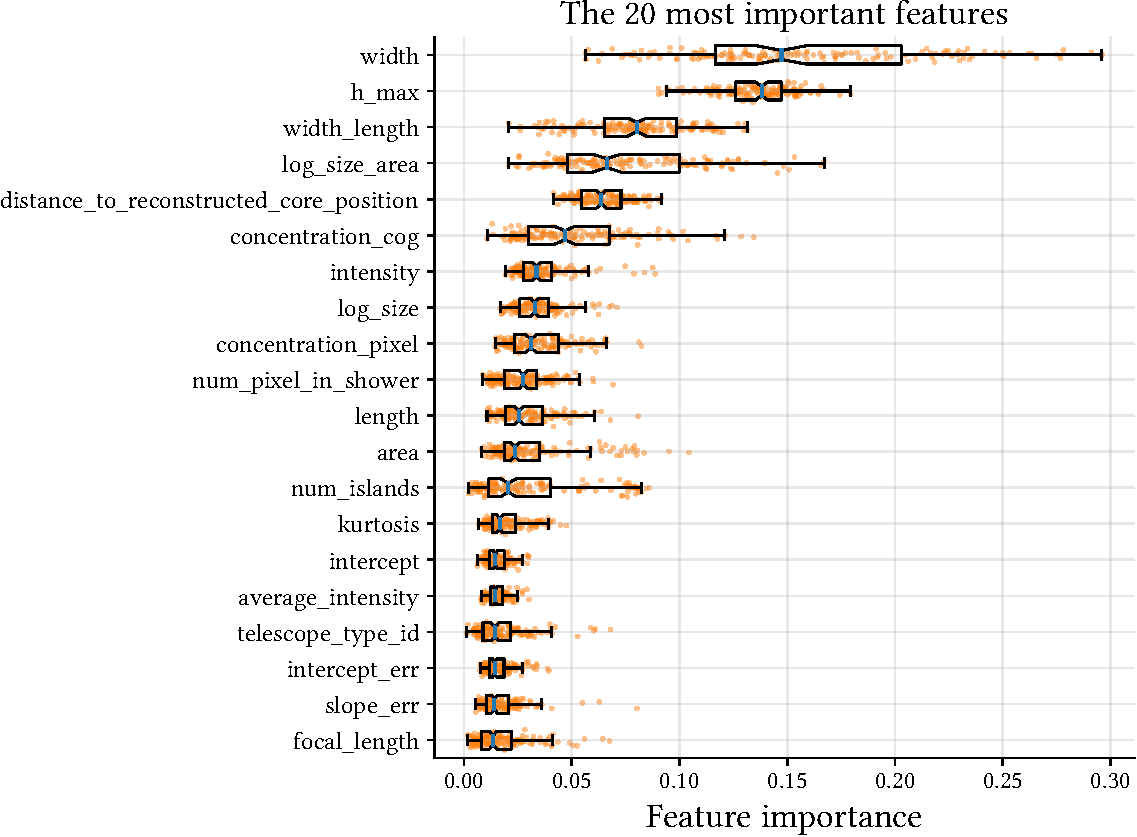
\includegraphics[page=1, width=.8\textwidth]{../analysis/plots/separation_features.pdf}
    \caption{Feature importance for the gamma/hadron separation.}
    \label{fig:gh_features}
\end{figure}


The resulting precision, recall and $f$-score are shown in figure \ref{fig:gh_fscore}.

\begin{figure}
    \centering
    \includegraphics[page=3, width=.8\textwidth]{../analysis/plots/cross_val_sep_perf_plot.pdf}
    \caption{Precision, recall and F-score for the gamma/hadron separation model on the 
    cross-validated dataset. The maximum F-score is achieved at a prediction threshold
    of $\approx \num{0.82}$.}
    \label{fig:gh_fscore}
\end{figure}

For the hadroness cut, that we apply later, we will choose the maximum of the $f_{\num{0.1}}$-score
at $\approx \num{0.82}$
% \chapter{energy}\label{energy}

ToDo:
\begin{enumerate}[nosep]
    \item Erklärung Features
    \item Trainingsperformance + daten
    \item Ergebnisse Mono
    \item Ergebnisse Stereo
\end{enumerate}

% \subsection{DISP and SIGN}
\label{energy}

The performance of the models trained with the previously mentioned setup,
can be gauged looking at 
figure \ref{fig:disp_perf}. For the DISP regressor model,
the R$^2$ score is chosen as a measure for performance. 
In the case of the SIGN classification model, it is the accuracy.
Both models perform better for higher event energies with accuracy and
R$^2$ reaching values close to 1.
At low energies the results do not seem to match the general trend.
Because the bins are chosen to be of equal width, they do not contain
comparable event counts especially at the lowest and highest energies.
This in combination with different telescopes triggering at different
energies explains the behaviour at those energies.
% For a plot with equally filled bins (of different width) have a look
% at the appendix \ref{app:plots}.

\begin{figure}
    \centering
    \captionsetup{width=0.9\linewidth}
    \begin{subfigure}{0.45\textwidth}
        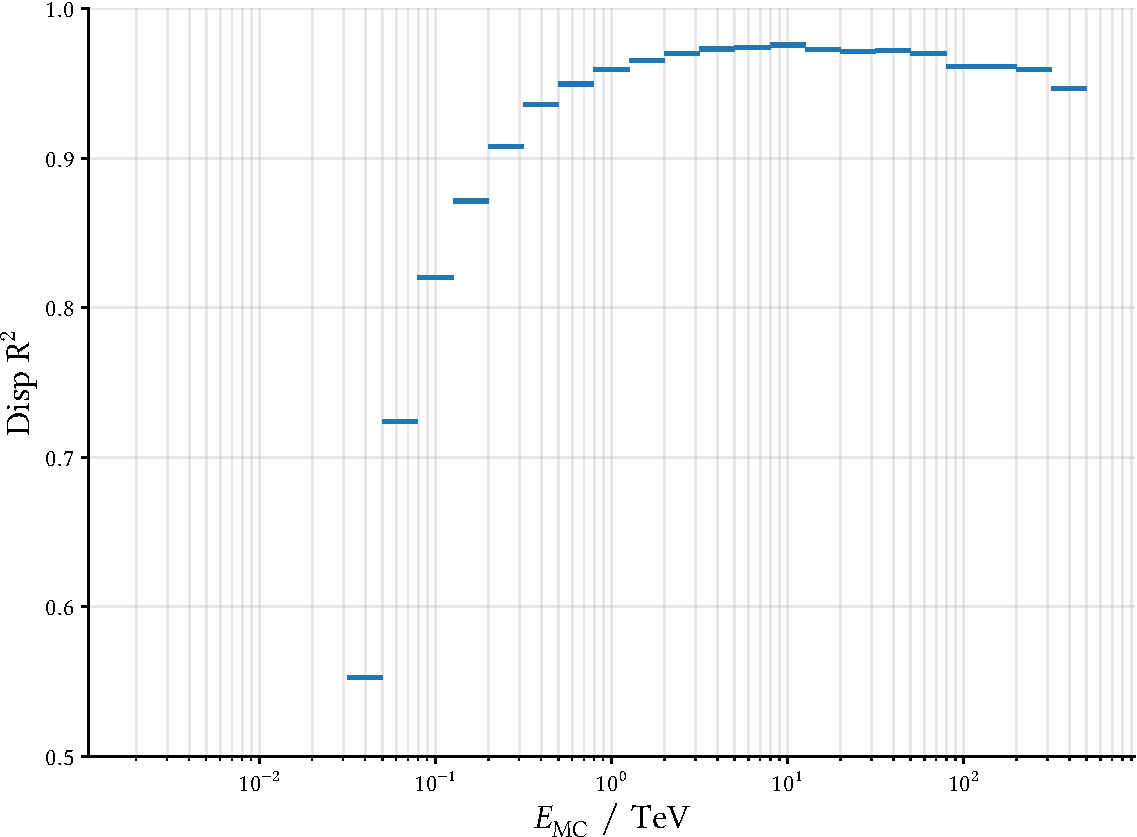
\includegraphics[width=\linewidth]{../analysis/plots/disp_gamma_r2_equal_sized.pdf} 
        \caption{R2-Score for the DISP-estimation}
    \end{subfigure}
    \begin{subfigure}{0.45\textwidth}
        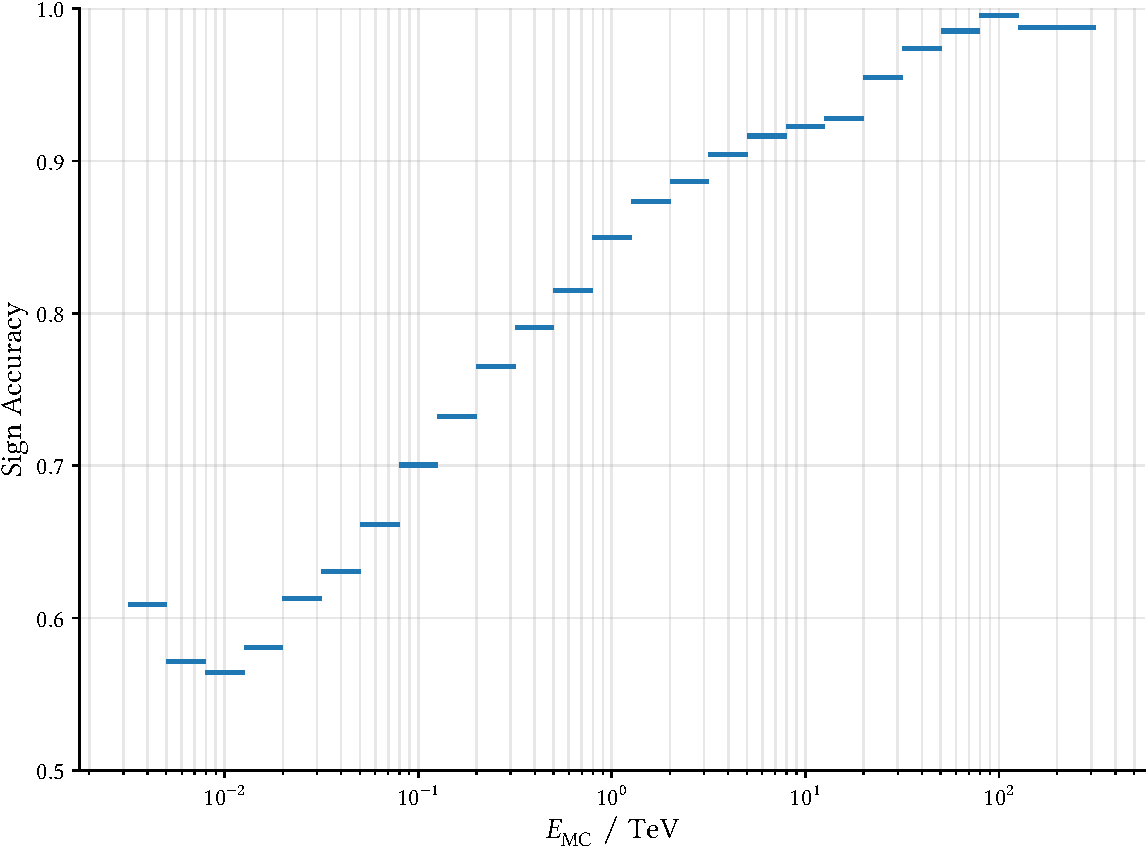
\includegraphics[width=\linewidth]{../analysis/plots/disp_gamma_acc_equal_sized.pdf}
        \caption{Accuracy for the SIGN-estimation}
    \end{subfigure}
    \caption{Performance of the DISP and SIGN model on the cross validated training
    data. In general both models performances improve with increasing energies.}
    % At low energies signs of overfitting can be noticed.}
    \label{fig:disp_perf}
\end{figure}

The feature importances are illustrated in the figures \ref{fig:disp_features}
for the DISP and \ref{fig:sign_features} for the SIGN model.
For the DISP model the stereoscopic features provide the most information.
Besides that, the light content, concentration and the length of the ellipse
are of most importance. Some separation into the different telescope types
seems to happen as well.
In the case of the SIGN model on the other hand, the predictions are almost
entirely based on the $skewness$ and $slope$ of the image.
The stereoscopic features do not provide much information in this case.
% which is expected as the head-/tail-ambiguation is entirely an artefact produced
% in the camera frame.

\begin{figure}
	\centering
    \captionsetup{width=0.9\linewidth}
	\hspace*{-0.11\textwidth}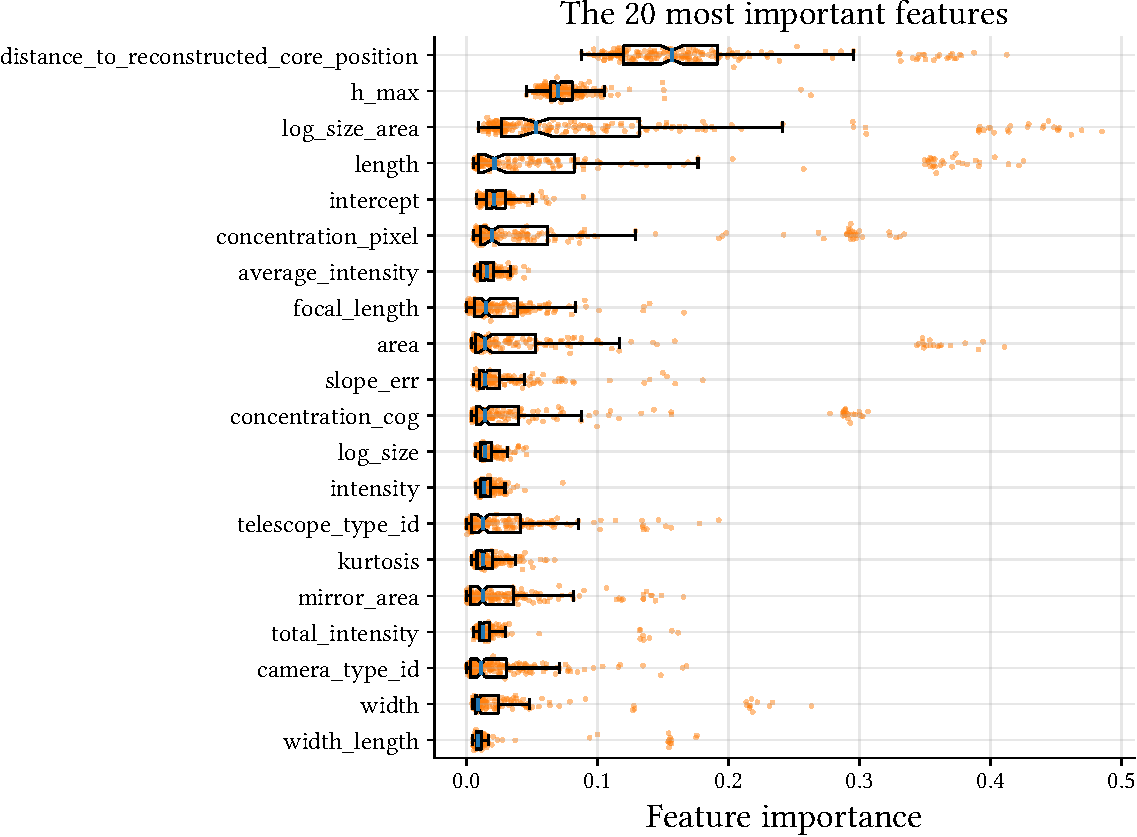
\includegraphics[width=0.6\textwidth]{../analysis/plots/disp_features.pdf}
	\caption{
	    Feature importance of the random forest for the DISP model.
	    The stereoscopic features have high influence on the prediction.
    	From the monoscopic features, the features describing the light content and the
        shape of the ellipse, provide most information.
        Additionaly the $concentration$-features, the $area$, $width$ and $length$
        are of high importance to the model.}
	\label{fig:disp_features}
\end{figure}

\begin{figure}
	\centering
    \captionsetup{width=0.9\linewidth}
	\hspace*{-0.1\textwidth}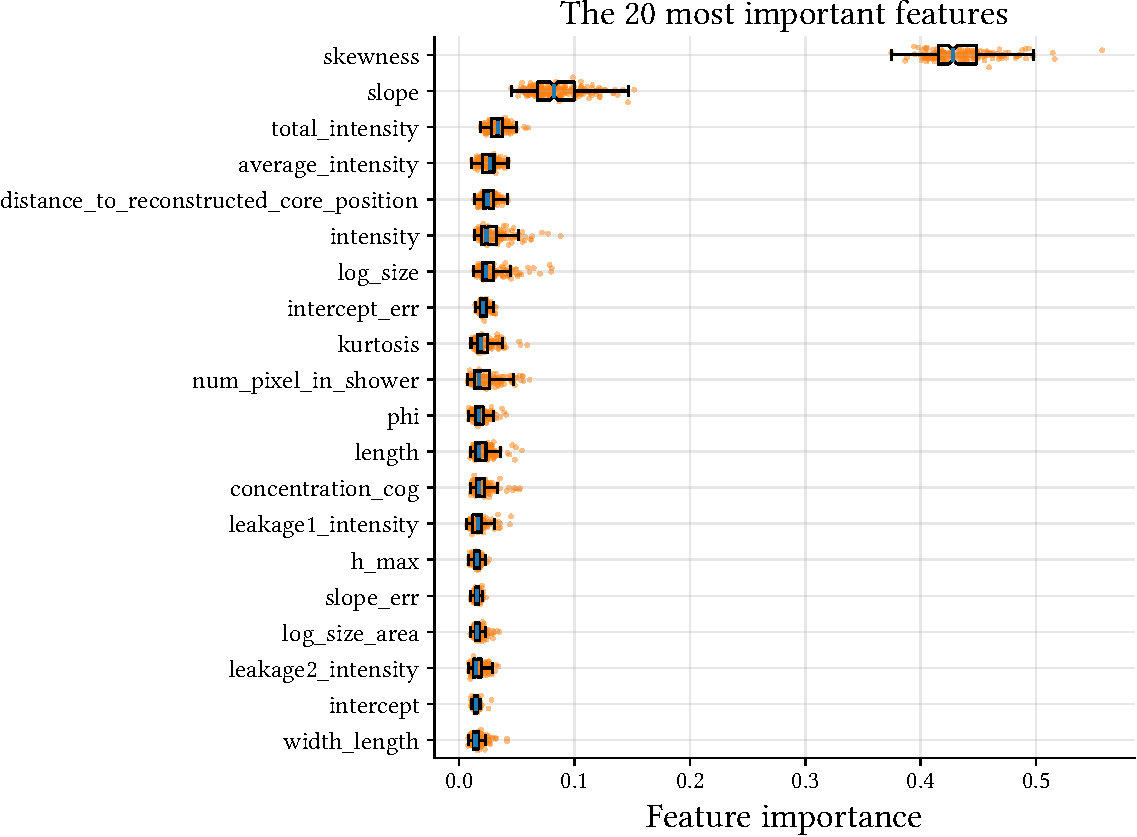
\includegraphics[width=0.6\textwidth]{../analysis/plots/sign_features.pdf}
	\caption{Feature importance of the random forest for the SIGN model.
	        The most influential features to the prediction are by far the higher-order moments $skewness$
            and $slope$. Other features provide very little information.}
	\label{fig:sign_features}
\end{figure}


% \section{Monoscopic Reconstruction}
\label{sec:mono}

% The performance of the models trained with the previously mentioned setup,
% can be gauged by looking at the 
% figures \ref{fig:disp_test_perf} for the diffuse test set and 
% \ref{fig:disp_gamma_perf} for the performance on the 
% pointlike data. For the DISP regressor model,
% the R2 score is chosen as a measure for performance. In the case of the SIGN classification model, it is
% the accuracy.

% In both cases, it can be noted, that the DISP-model gets rapidly more
% powerful with higher energies up until ~\SI{1}{\tera\electronvolt}. From 
% thereon, the performance does not improve anymore and in fact seems to decline
% again. For the diffuse test set, an additional dip around \SI{3}{\tera\electronvolt}
% up to \SI{70}{\tera\electronvolt} can be made out, that cannot
% be explained at this point.
% For pointlike gamma events the performance seems to decrease less at high energies.
% It does however hit a peak at $\SI{10}{\tera\electronvolt}$.

% The SIGN-model does not saturate early and improves up to the highest energies,
% apart from the very last bin.

% For both model, the performance on the pointlike data is generally better.
% This is expected as
% the sensitiviy is best in the middle of the camera.

% \begin{figure}
%     \centering
%     \captionsetup{width=0.9\linewidth}
%     \begin{subfigure}{0.45\textwidth}
%         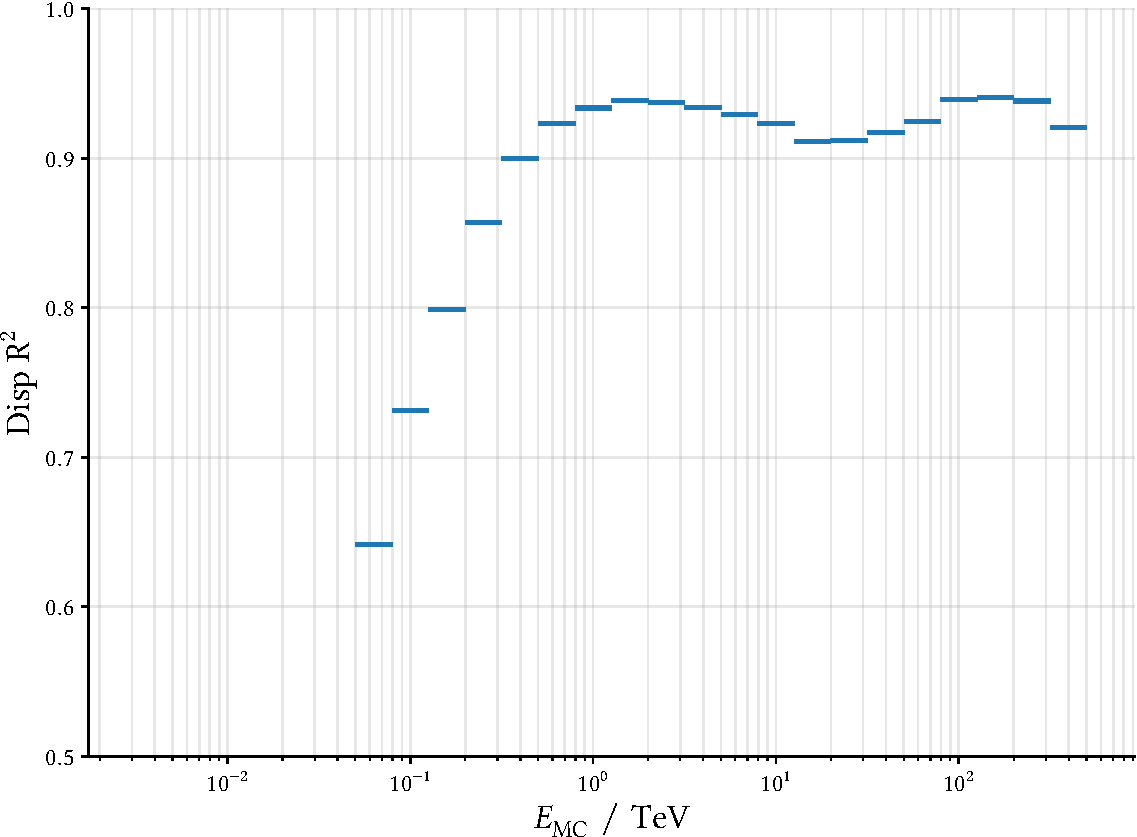
\includegraphics[width=\linewidth]{../analysis/plots/disp_test_r2_equal_sized.pdf} 
%         \caption{R2-Score for the DISP-estimation}
%     \end{subfigure}
%     \begin{subfigure}{0.45\textwidth}
%         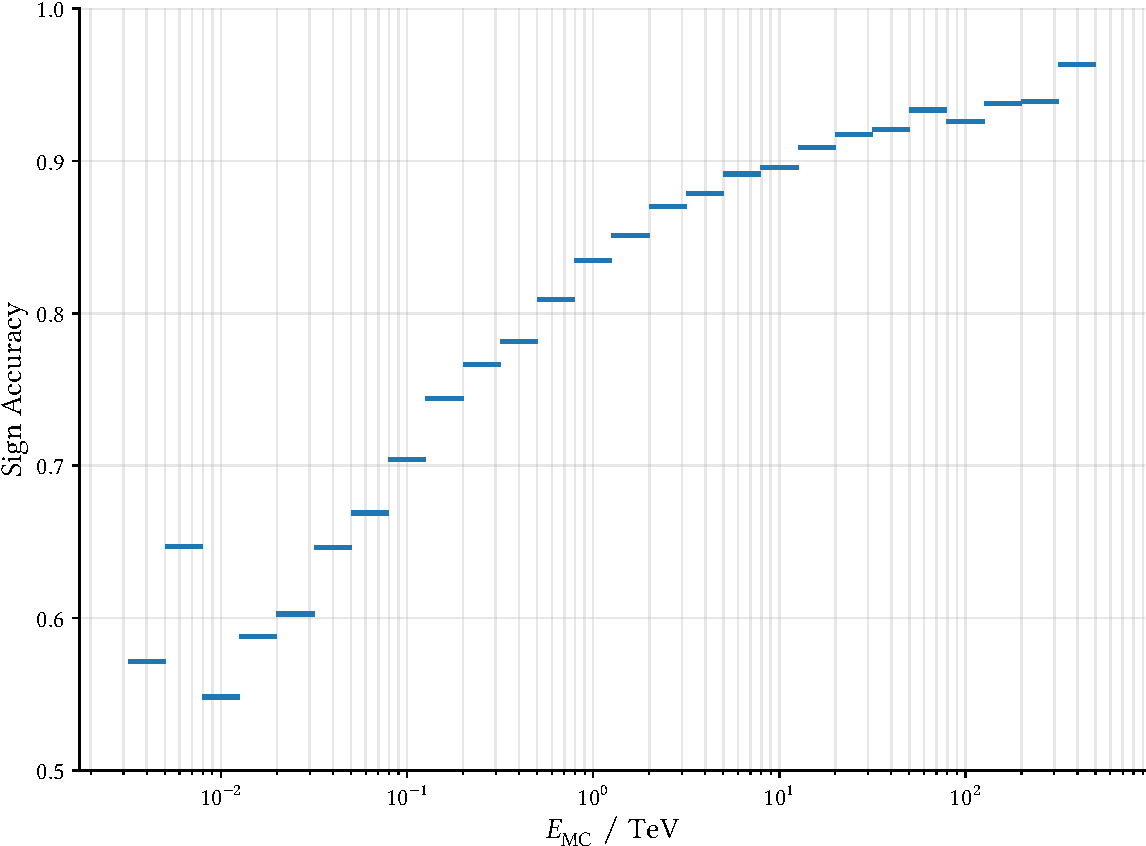
\includegraphics[width=\linewidth]{../analysis/plots/disp_test_acc_equal_sized.pdf}
%         \caption{Accuracy for the SIGN-estimation}
%     \end{subfigure}
%     \caption{
%     	Performance of the DISP- and SIGN-estimation algorithm on the diffuse test-dataset.
% 	Both model predictions improve with higher energies and saturate
% 	at $\approx\num{0.95}$ for the $R2$ and accuracy respectively.
%     The DISP-performance shows a dip in the energy range of \SI{3}{\tera\electronvolt}
%     up to \SI{70}{\tera\electronvolt}.}
%     \label{fig:disp_test_perf}
% \end{figure}

% \begin{figure}
%     \centering
%     \captionsetup{width=0.9\linewidth}
%     \begin{subfigure}{0.45\textwidth}
%         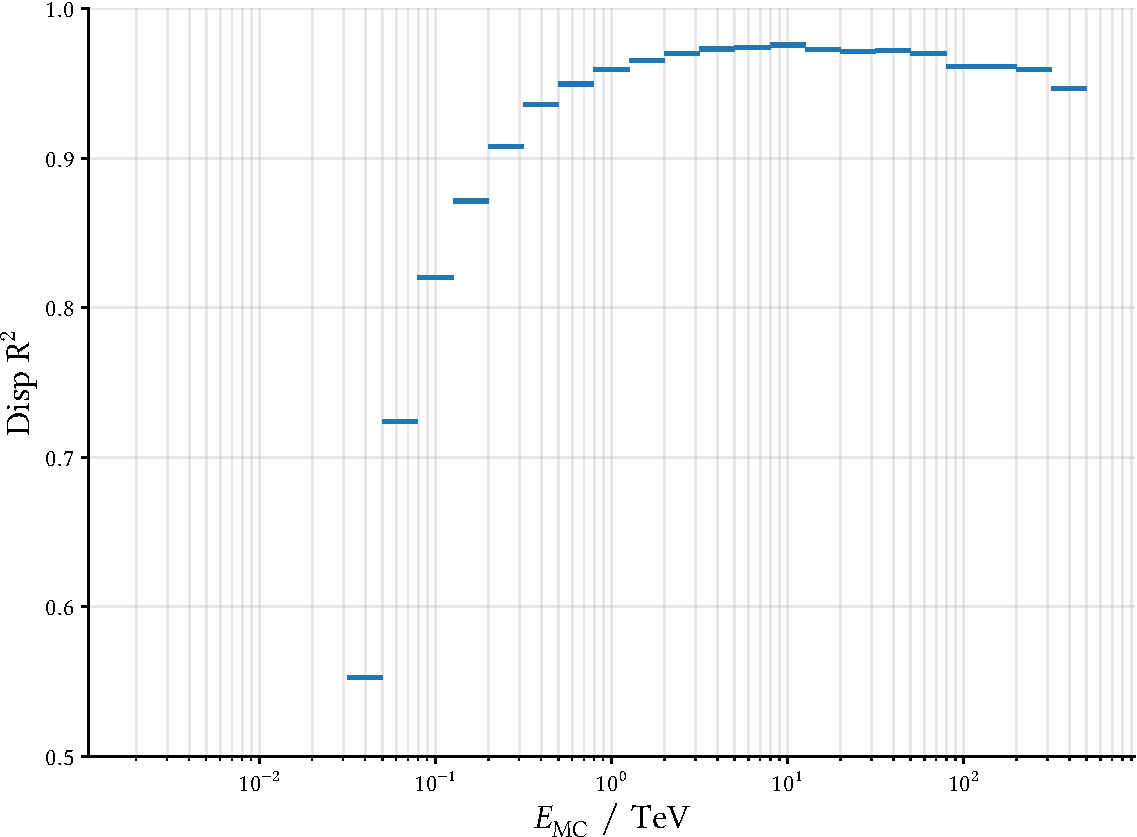
\includegraphics[width=\linewidth]{../analysis/plots/disp_gamma_r2_equal_sized.pdf} 
%         \caption{R2-Score for the DISP-estimation}
%     \end{subfigure}
%     \begin{subfigure}{0.45\textwidth}
%         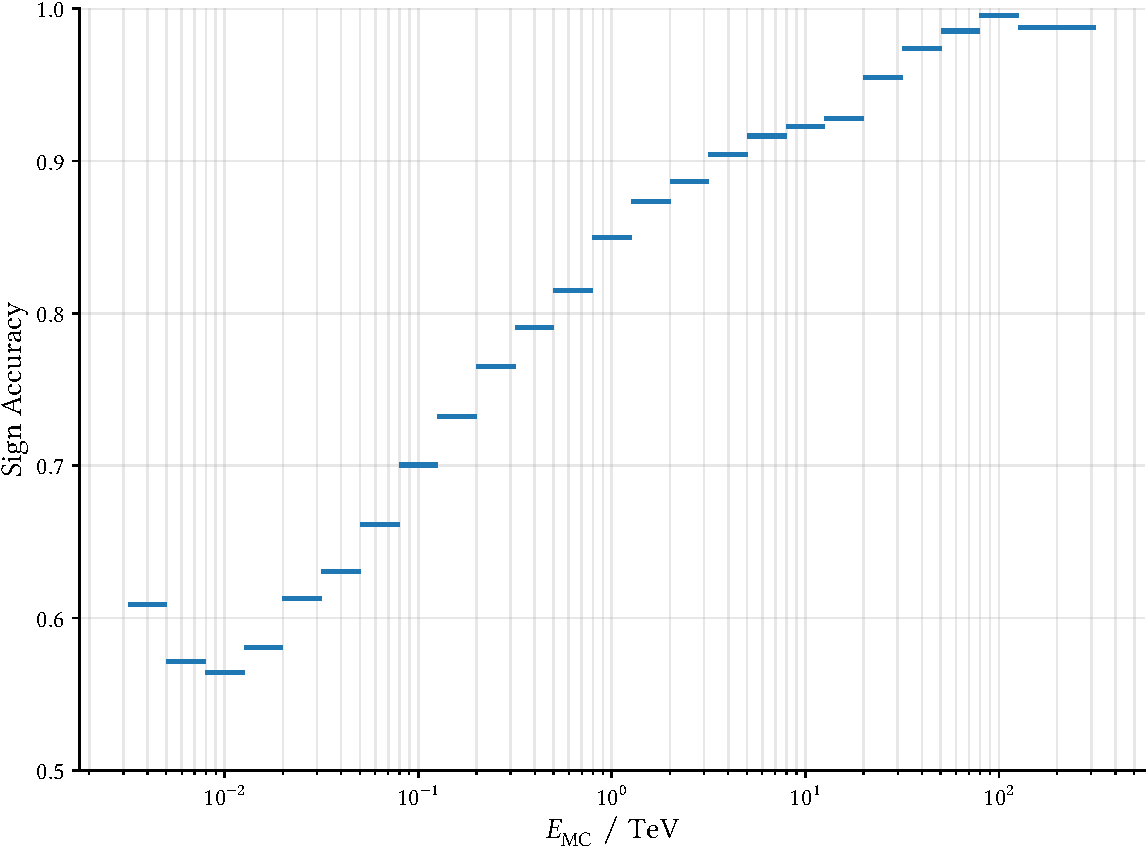
\includegraphics[width=\linewidth]{../analysis/plots/disp_gamma_acc_equal_sized.pdf}
%         \caption{SIGN-accuracy}
%     \end{subfigure}
%     \caption{
% 	Performance of the DISP- and SIGN-estimation algorithm on the pointlike dataset.
%     The R2-score of the DISP predictions shows a different form on pointlike
% 	compared to diffuse gammas: The performance generally is a bit better, 
% 	with saturation closer to 1. The dip at \SI{7}{\tera\electronvolt} is gone, but the highest energy bins
% 	show a decreasing performance.
%     The SIGN model performs similar, but the performance is slightly better throughout most of the energy range.}
%     \label{fig:disp_gamma_perf}
% \end{figure}
For the monoscopic reconstruction, all telescope events are taken as independent events and
the source position gets reconstructed using the DISP and SIGN model using the
pointlike gamma events.
Because events with misclasified SIGNs lead to predictions far away
from an assumed source position in a point source analysis of real data,
it can be argued to only keep events with properly reconstructed SIGNs.
In a real analysis, this would happen indirectly by performing a cut on 
the distance between assumed source position and reconstructed position.
On monte carlo data, we can just remove the events with misreconstructed SIGNs.
The angular resolution gets thus calculated with all reconstructed events and only with
the correctly reconstructed SIGNs.
This lowers the number of observed signal events,
but improves the angular resolution by a large margin.
Using only correctly assigned SIGNs on the pointlike dataset leaves 79\% of the events.
A sensitivity optimisation is not performed.

The angular resolution for all events
can be seen in figure \ref{fig:sens_telescope_gamma}.
Figure \ref{fig:sens_telescope_gamma_signs} shows only events with properly reconstructed SIGNs.
One can derive - in accordance to the previously discussed metrics - 
that both the DISP and SIGN predictions improve with increasing energies.
The predictions get worse at around the energies, where the $R2$-score
of the DISP-predictions saturates and decays.
Misreconstructed SIGNs are a problem expecially at low event energies as would be
expected from the accuracy of the SIGN model on the diffuse data.


% \begin{figure}
%     \centering
%     \captionsetup{width=0.9\linewidth}
%     \begin{subfigure}{0.45\textwidth}
%         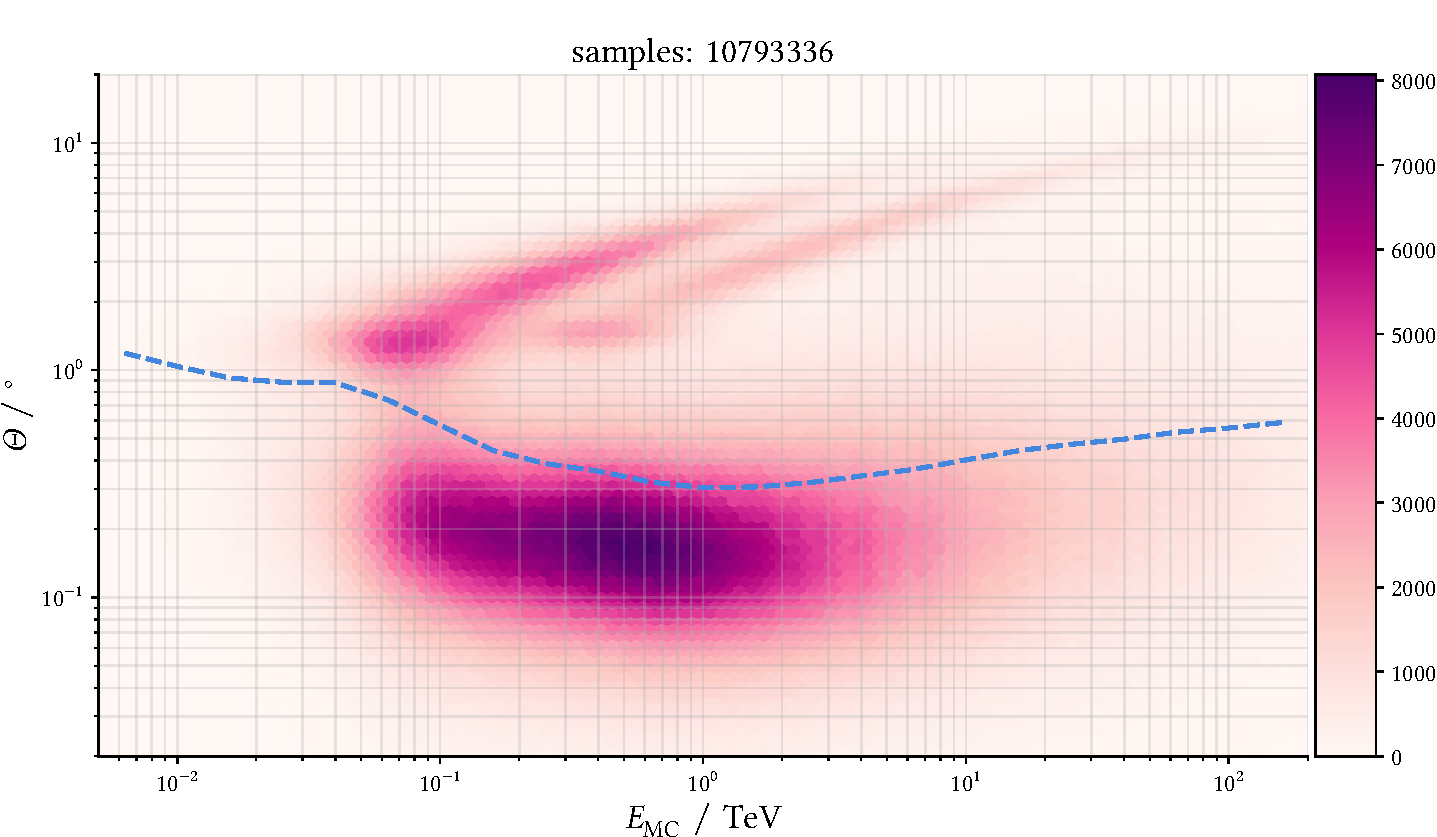
\includegraphics[width=0.6\textwidth]{../analysis/plots/test/tel_vs_energy.pdf}
%         \caption{All events}
%     \end{subfigure}
%     \begin{subfigure}{0.45\textwidth}
%         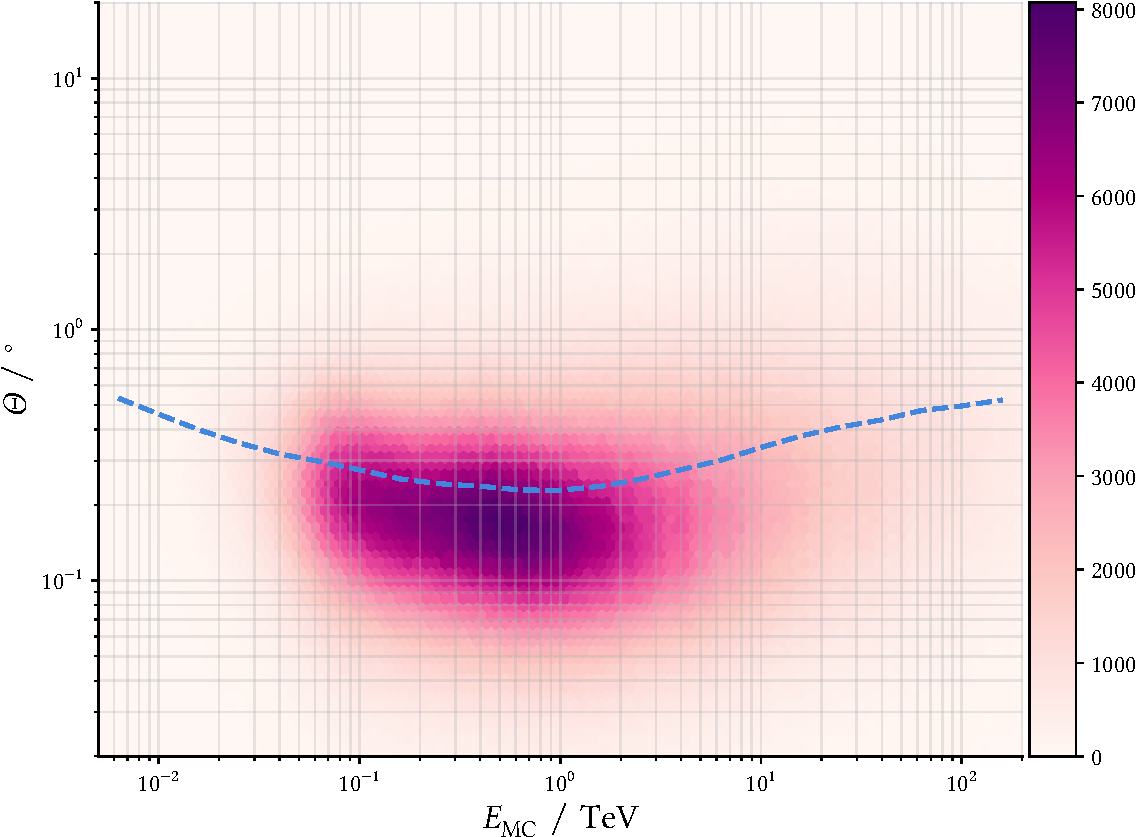
\includegraphics[width=0.6\textwidth]{../analysis/plots/test/tel_vs_energy_correct_signs.pdf}
%         \caption{Only correct SIGNs}
%     \end{subfigure}
%     \caption{
%         Monoscopic predictions for the source position on the pointlike 
%         test dataset with a total of XXX events. The blue-dotted line shows the 68\% containment. 
%         For lower energies, a big share of events has misreconstructed SIGNs,
%         leading to a second distribution with large $\Theta$. Upon removal of
%         the misclassified SIGNs, the 68\% containment on the
%         remaining XX events or XX\% is much improved.}
%     \label{fig:sens_telescope_test}
% \end{figure}

\begin{figure}
    \centering
    \captionsetup{width=0.9\linewidth}
    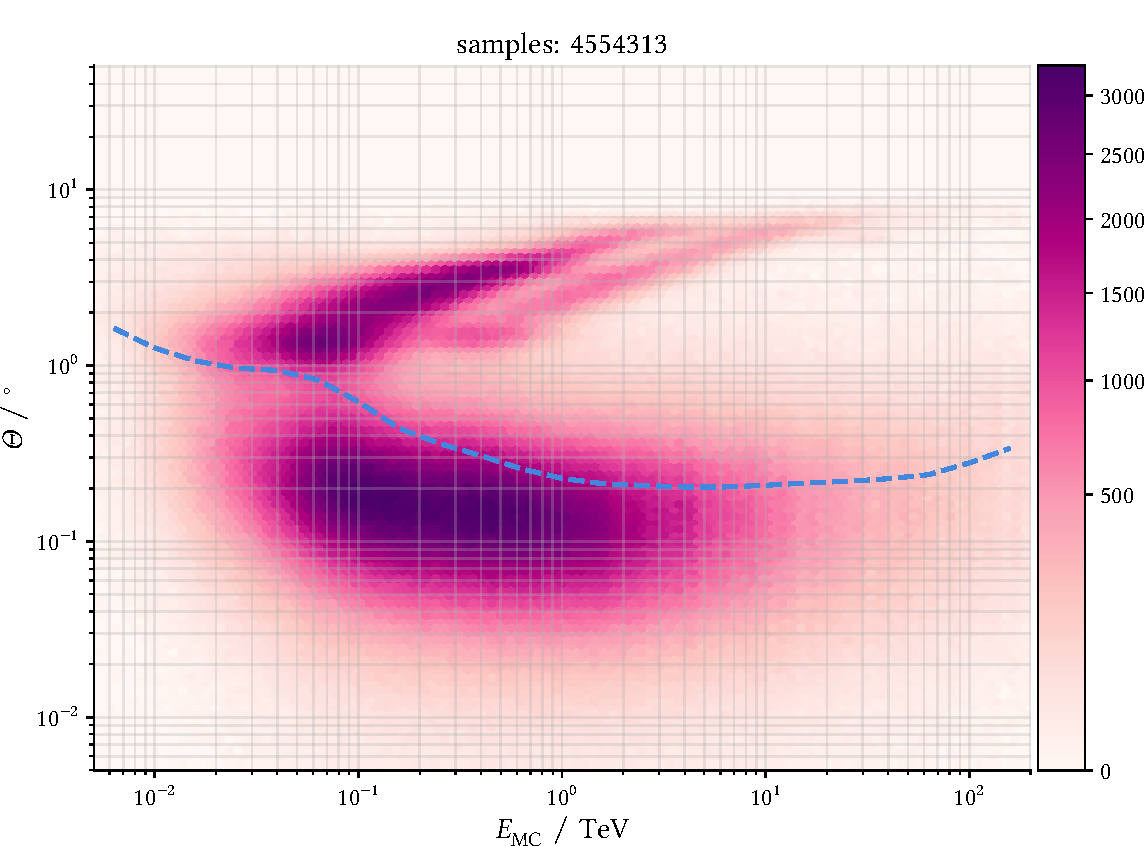
\includegraphics[width=0.6\textwidth]{../analysis/plots/gamma/tel_vs_energy.pdf}
    \caption{
        Monoscopic predictions for the source position on the pointlike 
        test dataset with a total of 4554313 telescope events.
        The blue-dotted line shows the 68\% containment. 
        For lower energies, a big share of events has misreconstructed SIGNs,
        leading to a second distribution with large $\Theta$.}
    \label{fig:sens_telescope_gamma}
\end{figure}


\begin{figure}
    \centering
    \captionsetup{width=0.9\linewidth}
    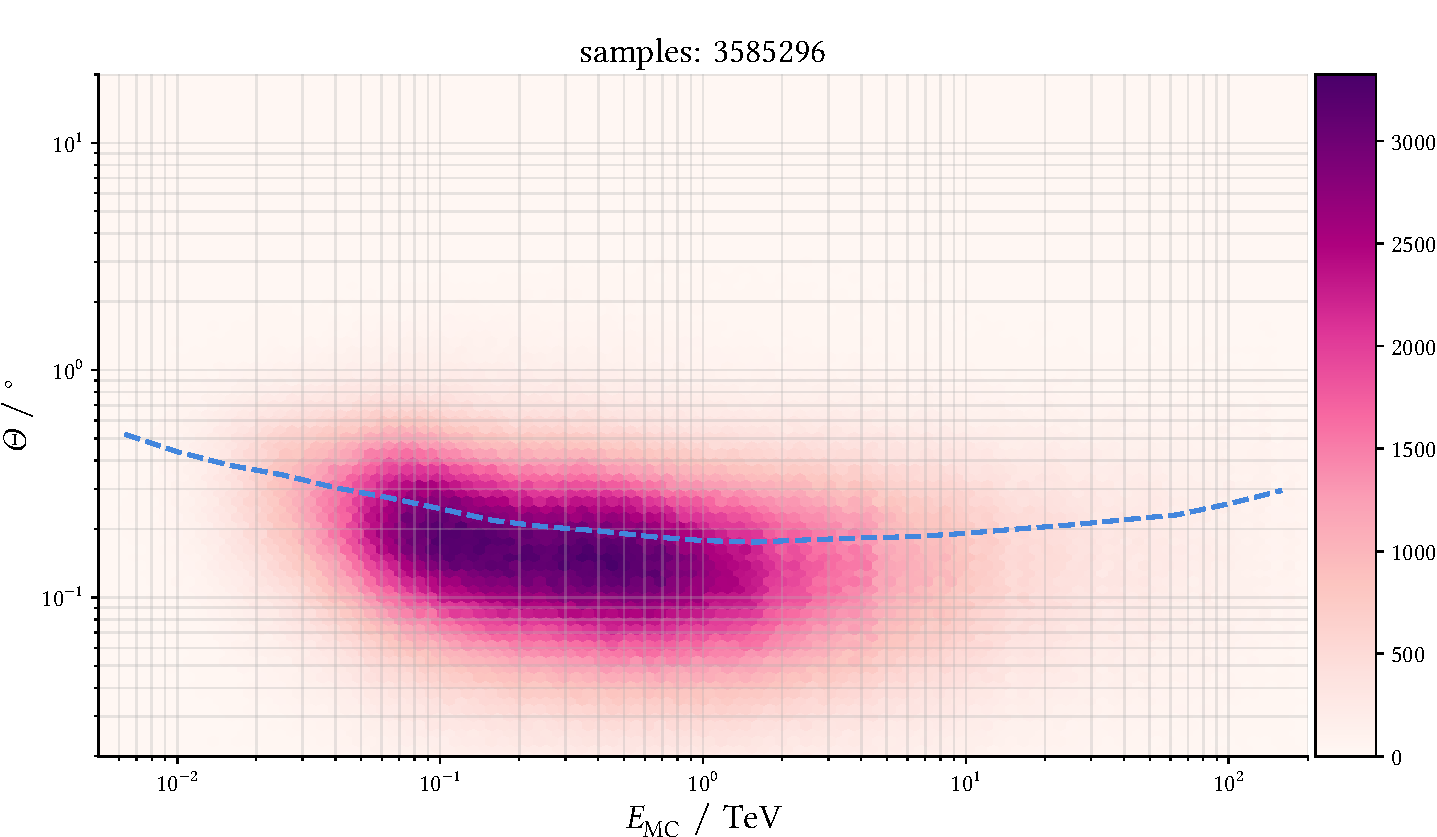
\includegraphics[width=0.6\textwidth]{../analysis/plots/gamma/tel_vs_energy_correct_signs.pdf}
    \caption{
        Monoscopic predictions for the source position on the pointlike 
        test dataset with a total of 3597952 events with properly reconstructed SIGNs. 
        The blue-dotted line shows the 68\% containment. 
        The angular resolution is much improved especially in the low energy regime
        where lots of events are removed.}
    \label{fig:sens_telescope_gamma_signs}
\end{figure}

% The feature importances for the DISP model can be seen in figure \ref{fig:disp_features},
% the one for the SIGN model in figure \ref{fig:sign_features}.
% For the DISP-model the reconstructed interaction heigth and core position
% show the most impact alongside the features, that describe the light content of
% the shower ellipse. The $length$ provides a lot of information whereas the
% $width$ is of little relevance for the prediction.
% The SIGN-predictions on the other hand are dominated by the observed 
% timing parameters $skewness$ and $slope$.

% \begin{figure}
% 	\centering
%     \captionsetup{width=0.9\linewidth}
% 	\hspace*{-0.15\textwidth}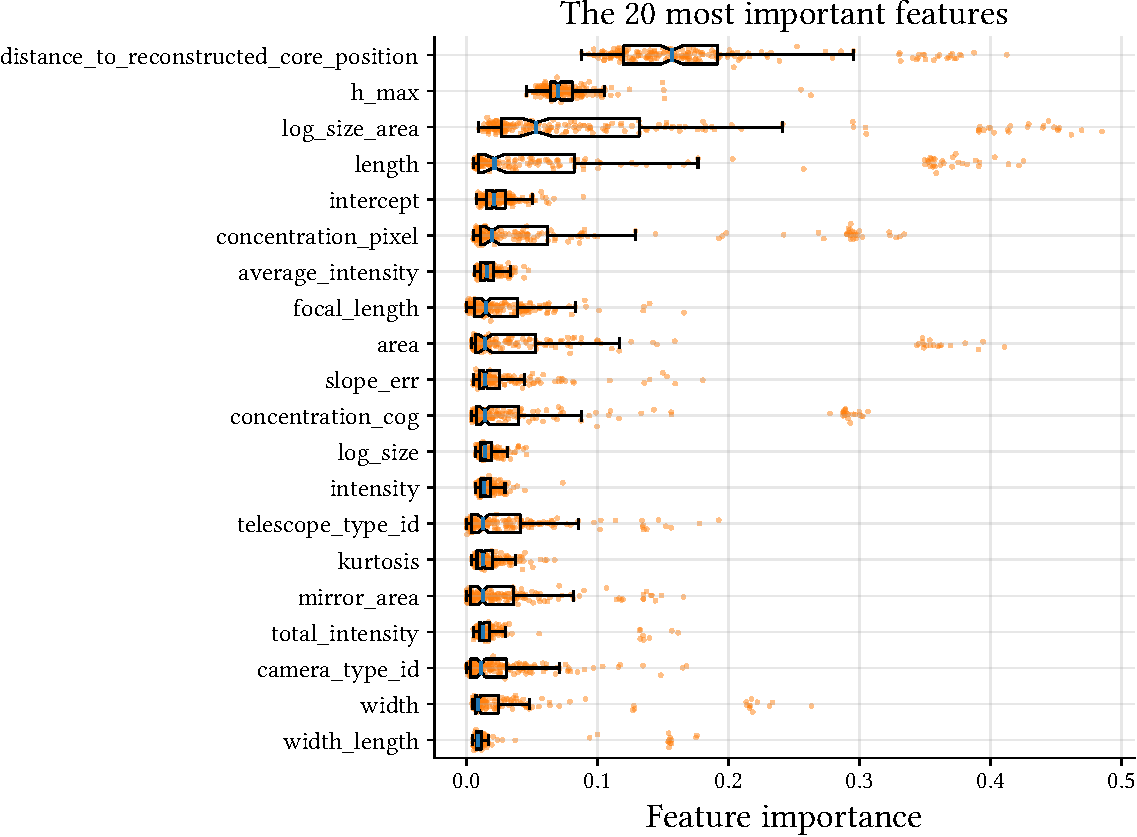
\includegraphics[width=0.6\textwidth]{../analysis/plots/disp_features.pdf}
% 	\caption{
% 	    Feature importance of the random forest for the DISP model.
% 	    The stereoscopic features have high influence on the prediction.
%     	From the monoscopic features, the features describing the light content and the
%         shape of the ellipse, provide most information.
%         Looking at the distribution of the individual feature importances, it 
%         can be derived that the range of important featrues is bigger than this list
%         with especially the $concentration$-features, the $area$, $width$ and $length$
%         being of high importance to the model as well.}
% 	\label{fig:disp_features}
% \end{figure}

% \begin{figure}
% 	\centering
%     \captionsetup{width=0.9\linewidth}
% 	\hspace*{-0.15\textwidth}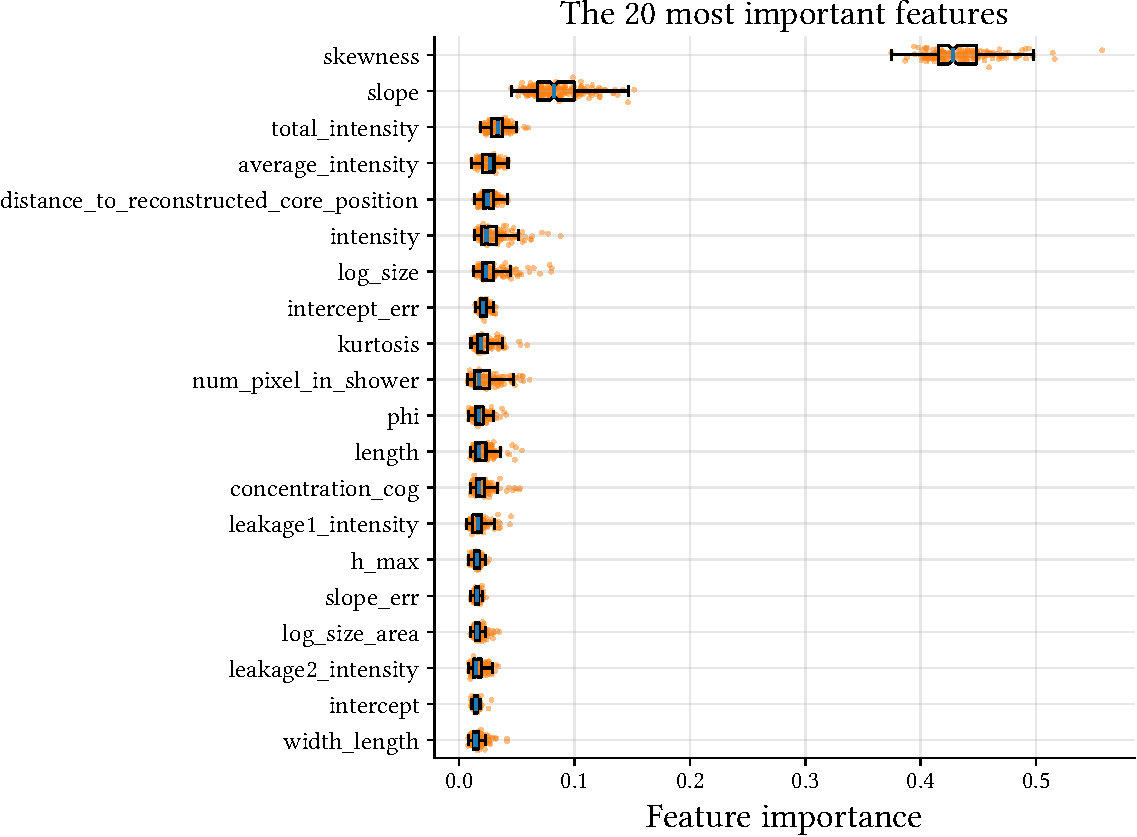
\includegraphics[width=0.6\textwidth]{../analysis/plots/sign_features.pdf}
% 	\caption{Feature importance of the random forest for the SIGN model.
% 	        The most influential features to the prediction are by far the higher-order moments $skewness$
%             and $slope$. The stereoscopic features do not provide much information,
%             which is expected as the head-/tail-ambiguation is entirely an artefact produced
%             in the camera frame. Other features provide very little information.}
% 	\label{fig:sign_features}
% \end{figure}


\section{Stereoscopic Reconstruction}\label{position}

Using the models mentioned in \ref{sec:mono}, the resulting DISP+SIGN predictions
are combined transforming the predictions to the nominal frame and then
transforming the median in the nominal frame to the horizon frame.
The angular resolution over the true event energy of this baseline stereoscopic predictions
compared to the existing HillasReconstructor can be seen in figure \ref{fig:stereo_median_energy}.
The angular resolution against the event multiplicity is displayed in figure \ref{fig:stereo_median_multi}.

At each energy, the HillasReconstructor performs considerably better.
One can derive that the median predictions do not improve considerably above
\SI{3}{\tera\electronvolt} and get worse above \SI{10}{\tera\electronvolt}.
The HillasReconstructor shows a saturation at the highest energies,
but without the prominently decaying performance of the median predictions.
It can also be noted, that the median predictions seem to not completely
resolve the problem with wrong SIGNs.

Looking at the performance over the event multiplicity we can conclude that the median predictions
do not scale as well with higher multiplicities, so that the performance gap increases with
the multiplicities going up.

The HillasReconstructor also shows a pronounced bump in the range of \SI{200}{\giga\electronvolt}
to \SI{1}{\tera\electronvolt}. 
This can be connected to a high number of low multiplicity events in the
LST-MST crossover region, which limits the performance.
% This has been observed in other analyses as well and seems to correlate with 
% a lot of low multiplicity events in the crossover region from LSTs to MSTs \cite{kai? max?}.

\begin{figure}
    \centering
    \captionsetup{width=0.9\linewidth}
    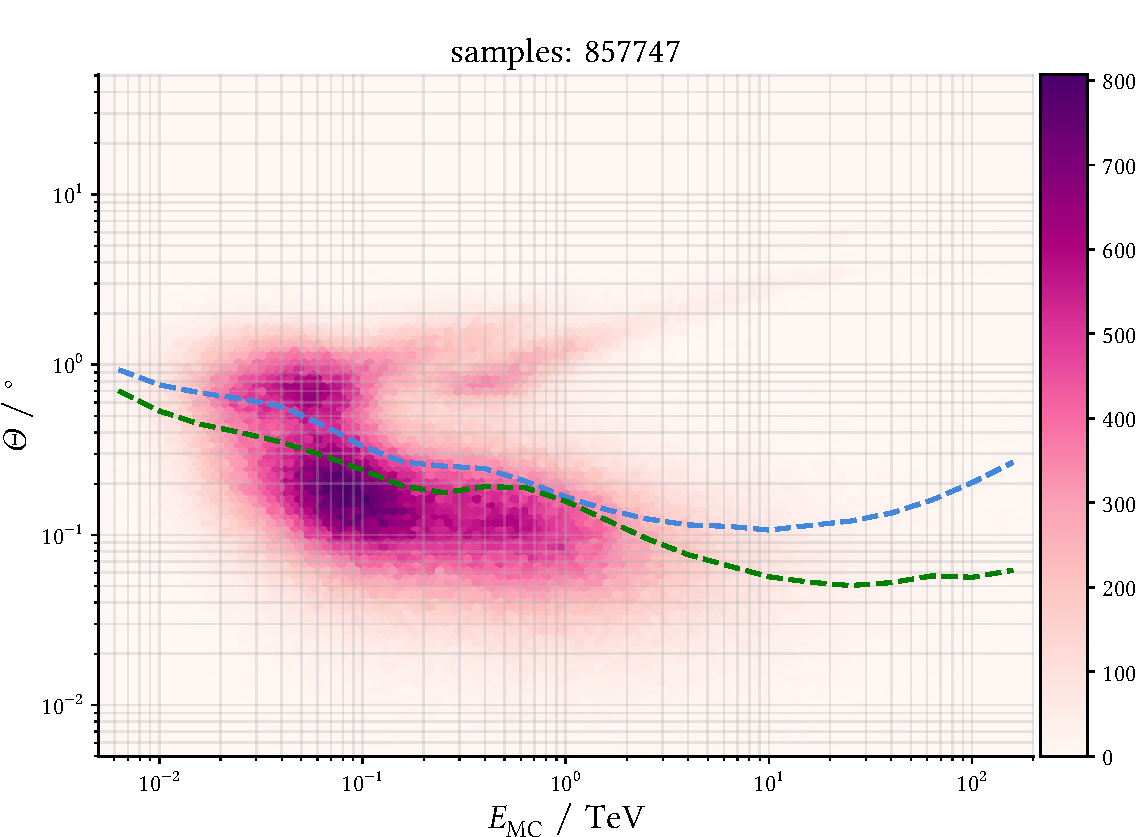
\includegraphics[width=0.6\textwidth]{../analysis/plots/gamma/median_vs_energy.pdf} 
    \caption{Distance between predicted and true position over true energy as obtained by taking the median of
    the DISP+SIGN predictions on 955317 pointlike gamma events. The blue line shows the 
    68\% containment of these results. The green line refers to the 68\%
    results of the HillasReconstructor, which is added for comparison, but has no
    connection to the binned results.
    Despite the short bump in the range of \SI{200}{\giga\electronvolt}
    to \SI{1}{\tera\electronvolt} the HillasReconstructor outperforms the median predictions
    massively.}
    \label{fig:stereo_median_energy}
\end{figure}

\begin{figure}
    \centering
    \captionsetup{width=0.9\linewidth}
    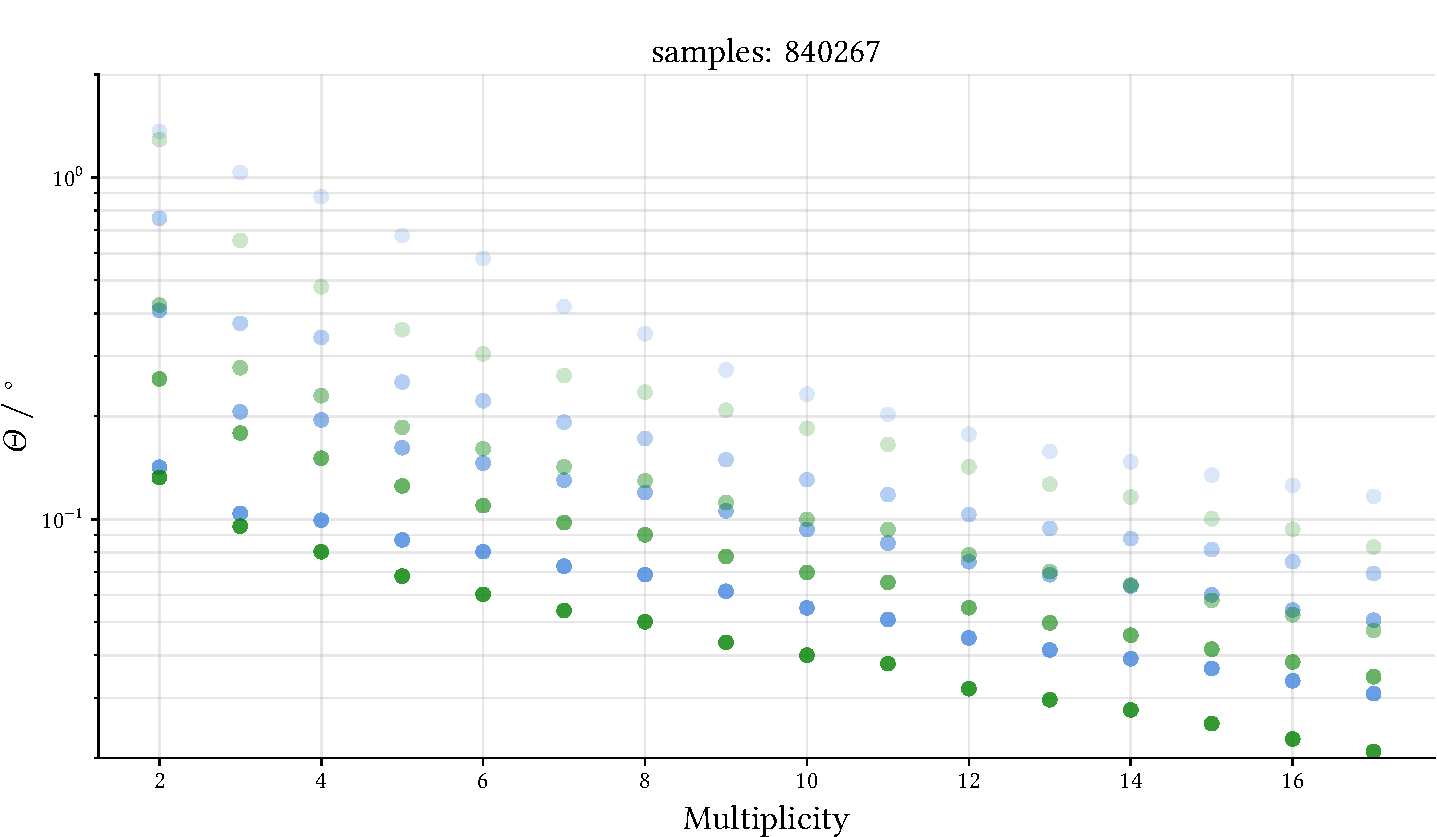
\includegraphics[width=0.6\textwidth]{../analysis/plots/gamma/median_vs_multi_comp.pdf}
    \caption{Distance between predicted and true position over event multiplicity as obtained by taking
    the median, if the DISP+SIGN predictions (blue) and using the HillasReconstructor (green)
    on 955317 pointlike gamma events. 
    The different dots refer to the 25, 50, 68 and 90\% percentiles with 
    lowering opacity.
    The median predictions are worse at every multiplicity and the gap increases with higher event multiplicity.}
    \label{fig:stereo_median_multi}
\end{figure}

The results of the iterative DISP-approach can be seen in figures
\ref{fig:stereo_magic_energy} and \ref{fig:stereo_magic_multi}.
Compared to the median predictions, the 68\% percentile is much improved throughout the complete energy range besides 
the very highest energies. At this point the error of the DISP-predictions is probably limiting and the 
HillasReconstructor leads to much better results.
At the lower energy range the approach seems to be working well, outperforming the HillasReconstructor.

When looking at the multiplicity dependency, we see improved results as well. 
At high event multiplicities the Hillas-reconstructor still
leads to better results. At low multiplicites on the other hand,
especially at 2- and 3-multiplicity events, the apporach works very well.
The HillasReconstructor starts to outperform at multiplicities of 4-6.

\begin{figure}
    \centering
    \captionsetup{width=0.9\linewidth}
    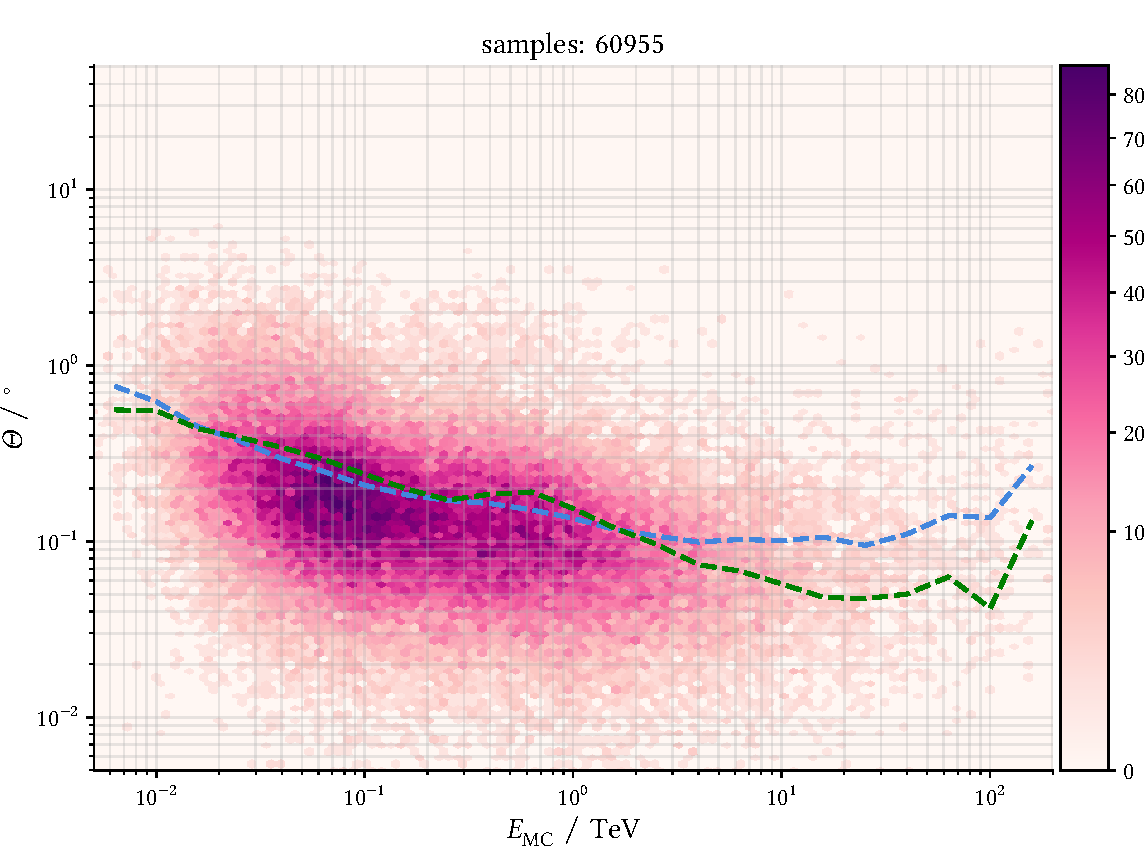
\includegraphics[width=0.6\linewidth]{../analysis/plots/gamma/pairwise_median_100_vs_energy.pdf} 
    \caption{Distance between predicted and true position over true event energy as obtained with the
    iterative DISP approach on 955317 pointlike gamma events.
    The binned results refer to the iterative DISP-predictions. The blue line shows the 
    68\% containment of these results. The green line refers to the 68\%
    results of the HillasReconstructor.
    The DISP-approach outperforms the HillasReconstructor up to
    $\approx \SI{2}{\tera\electronvolt}$.}
    \label{fig:stereo_magic_energy}
\end{figure}

\begin{figure}
    \centering
    \captionsetup{width=0.9\linewidth}
    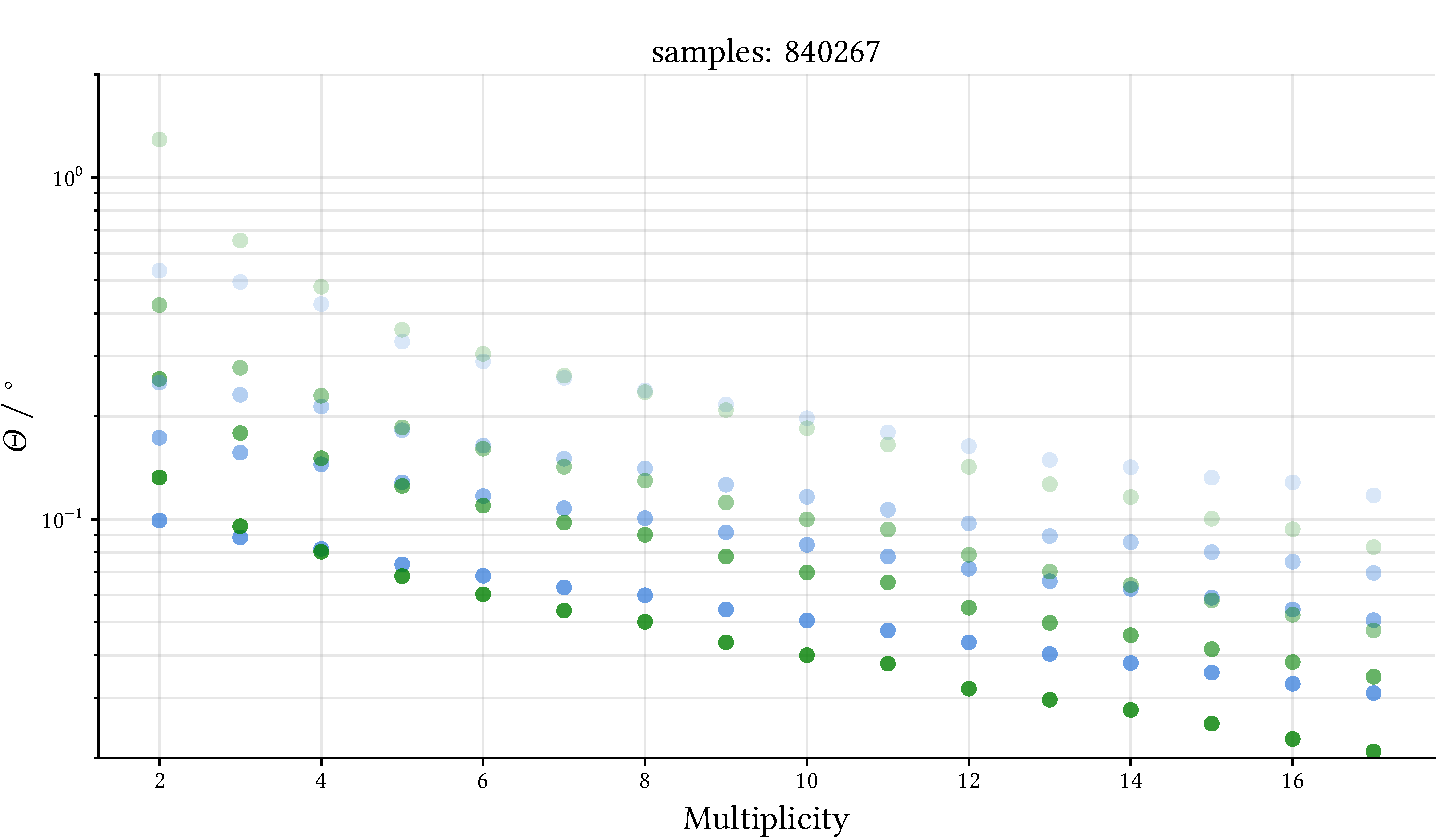
\includegraphics[width=0.6\linewidth]{../analysis/plots/gamma/pairwise_median_100_vs_multi_comp.pdf}
    \caption{Distance between predicted and true position over event multiplicity as obtained with
    the iterative DISP approach (blue) and the HillasReconstructor (green)
    on 955317 pointlike gamma events.
    The different lines refer to the 25,50,68 and 90\% percentiles with 
    lowering opacities.
    For low multiplicities, the combined DISP-predictions are superiour, 
    for high multiplicities the HillasReconstructor results win out.
    The breakeven point seems to be at 4-6 telescopes, depending on 
    which percentiles have more weight to the analysis.}
    \label{fig:stereo_magic_multi}
\end{figure}

\section{Stereoscopic Sensitivities}

Two independent sensitivity optimisations are being performed,
one for the HillasReconstructor analysis and one for the stereoscopic DISP analysis.
The background separation and energy models are the same in both cases
as are the preprocessed datasets.
The pointlike gamma data acts as signal events, the background is formed by
the proton test set. The results get compared
to the CTA reference analysis \cite{cta_web}.
Details of the reference analysis have not been shared.
In this case it merely included as a naive benchmark, because
comparability can not be assumed.
For the same reason and with the same limitations
the CTA requrements are included as well.
Even If nothing else, the purely protonic background is a large simplification
and the background statistic in general seems to be too low to
provide proper sensitivities. 

Starting with the HillasReconstructor, the prediction
and theta cut get optimized in each bin of energy performing a gridsearch on the 
values of the event multiplicity, $\Theta$ and prediction threshold.
The possible range of values is:

$$ \Theta: 0.01, 0.02, \ldots, 0.17 $$
$$ \text{prediction threshold} \alpha: 0.5, 0.55, \ldots, 1.00 $$
$$ \text{multiplicity}: 2, 3, \ldots, 10 $$

Best sensitivities get achieved with the following parameter combination:

% \afterpage{
%     \thispagestyle{empty}
%     \begin{landscape}
%         %\caption{Optimized cuts for the Hillasreconstructor analysis in logarithmic energy bins.
%         %The event counts correspond to the counts after weighting.}
%         %\begin{center}
%             \centering
%             \begin{tabular}{c c c c c r c c}
%                 %\hline
%                 $E_\text{min}$ / \si{\tera\electronvolt} & $E_\text{max}$ / \si{\tera\electronvolt} & $\alpha$ & $\Theta$ & Mult. & Sign. & sig counts & bkg counts \\
%                 \hline
%                 \num{0.02} & \num{0.03} & 0.75 & 0.12 & 2 & \num{67.081609668104} & \num{12684.82} (\num{3119}) & \num{125557.82} (\num{476})\\
%                 \num{0.03} & \num{0.05} & 0.6 & 0.17 & 2 & \num{143.914706929475} & \num{58145.94} (\num{13840}) & \num{572791.75} (\num{1214}) \\
%                 \num{0.05} & \num{0.08} & 0.6 & 0.17 & 2 & \num{327.902927338685} & \num{166199.76} (\num{38918}) & \num{774710.40} (\num{2032}) \\
%                 \num{0.08} & \num{0.12} & 0.6 & 0.16 & 2 & \num{466.286269748645} & \num{160335.10} (\num{38495}) & \num{234553.03} (\num{852}) \\
%                 \num{0.13} & \num{0.20} & 0.7 & 0.11 & 6 & \num{404.026953731173} & \num{58324.53} (\num{14379}) & \num{9678.95} (\num{83}) \\
%                 \num{0.20} & \num{0.32} & 0.8 & 0.09 & 6 & \num{291.173501331132} & \num{24694.15} (\num{6922}) & \num{404.89} (\num{6}) \\
%                 \num{0.32} & \num{0.50} & 0.8 & 0.08 & 10 & \num{278.308880907216} & \num{21899.35} (\num{6949}) & \num{84.86} (\num{2}) \\
%                 \num{0.50} & \num{0.80} & 0.8 & 0.07 & 6 & \num{301.554242885264} & \num{25516.59} (\num{9771}) & \num{35.88} (\num{2}) \\
%                 \num{0.80} & \num{1.26} & 0.8 & 0.06 & 7 & \num{238.800568473337} & \num{16000.56} (\num{7552}) & \num{22.20} (\num{2}) \\
%                 \num{1.26} & \num{2.00} & 0.75 & 0.05 & 10 & \num{193.005662032815} & \num{10450.36} (\num{6207}) & \num{13.98} (\num{2}) \\
%                 \num{2.00} & \num{3.17} & 0.75 & 0.06 & 6 & \num{189.144224666632} & \num{10008.57} (\num{8098}) & \num{5.70} (\num{1}) \\
%                 \num{3.17} & \num{5.02} & 0.7 & 0.05 & 7 & \num{140.184997871284} & \num{5512.73} (\num{6114}) & \num{7.27} (\num{3}) \\
%                 \num{5.02} & \num{7.96} & 0.7 & 0.05 & 9 & \num{97.3831573129413} & \num{2656.42} (\num{4223}) & \num{2.40} (\num{1}) \\
%                 \num{7.96} & \num{12.62} & 0.7 & 0.06 & 6 & \num{79.3212652969814} & \num{1764.58} (\num{4219}) & \num{2.21} (\num{1}) \\
%                 \num{12.62} & \num{20.00} & 0.65 & 0.05 & 4 & \num{56.0187708296887} & \num{899.54} (\num{3306}) & \num{8.42} (\num{6}) \\
%                 \num{20.00} & \num{31.70} & 0.6 & 0.06 & 5 & \num{38.4920204879829} & \num{417.91} (\num{2431}) & \num{1.27} (\num{1}) \\
%                 \num{31.70} & \num{50.24} & 0.55 & 0.07 & 3 & \num{27.1123543279959} & \num{210.29} (\num{2063}) & \num{1.76} (\num{1}) \\
%                 \num{50.24} & \num{72.62} & 0.45 & 0.07 & 3 & \num{17.4720214115349} & \num{88.46} (\num{1526}) & \num{1.24} (\num{1}) \\
%                 \num{79.62} & \num{126.19} & 0.45 & 0.07 & 2 & \num{9.47422298618942} & \num{27.84} (\num{865}) & \num{1.45} (\num{2}) \\
%                 \num{126.19} & \num{200.00} & 0.35 & 0.17 & 2 & \num{3.52411688223802} & \num{10.01} (\num{578}) & \num{17.27} (\num{5}) \\
%             %\hline
%             \end{tabular}
%         %\end{center}
%         %\label{tab:hillas_cuts}
%     \end{landscape}
% }
% \clearpage


%\KOMAoptions{paper=landscape,pagesize}
%\recalctypearea
\newpage
\storeareas\normalsetting
\KOMAoption{paper}{landscape}
\areaset{4\textwidth}{.9\textheight}
\recalctypearea
    \centering
    %\captionsetup{width=0.9\linewidth}
    \captionof{table}{Thresholds, significances and event counts for the sensitivity curve of the
    HillasReconstructor analysis. The event counts related to the weighted events. The unweighted event counts are given
    in brackets behind.}
    \begin{tabular}{r r r r r r r r c }
        %\hline
        $E_\text{min}$ / \si{\tera\electronvolt} & $E_\text{max}$ / \si{\tera\electronvolt} & $\alpha$ & $\Theta$ & Multiplicity & Sign. &  \multicolumn{2}{| c |}{test} & Bkg Counts \\
        \hline
        \num{0.02} & \num{0.03} & 0.75 & 0.12 & 2 & \num{67.08} & \num{12684.82} & \num{3119} & \num{125557.82} (\num{476})\\
        \num{0.03} & \num{0.05} & 0.6 & 0.17 & 2 & \num{143.91} & \num{58145.94} & \num{13840} & \num{572791.75} (\num{1214}) \\
        \num{0.05} & \num{0.08} & 0.6 & 0.17 & 2 & \num{327.90} & \num{166199.76} & \num{38918} & \num{774710.40} (\num{2032}) \\
        \num{0.08} & \num{0.12} & 0.65 & 0.16 & 2 & \num{466.29} & \num{160335.10} & \num{38495} & \num{234553.03} (\num{852}) \\
        \num{0.13} & \num{0.20} & 0.7 & 0.11 & 6 & \num{404.03} & \num{58324.53} & \num{14379} & \num{9678.95} (\num{83}) \\
        \num{0.20} & \num{0.32} & 0.8 & 0.09 & 6 & \num{291.17} & \num{24694.15} & \num{6922} & \num{404.89} (\num{6}) \\
        \num{0.32} & \num{0.50} & 0.8 & 0.08 & 10 & \num{278.31} & \num{21899.35} & \num{6949} & \num{84.86} (\num{2}) \\
        \num{0.50} & \num{0.80} & 0.8 & 0.07 & 6 & \num{301.55} & \num{25516.59} & \num{9771} & \num{35.88} (\num{2}) \\
        \num{0.80} & \num{1.26} & 0.8 & 0.06 & 7 & \num{238.80} & \num{16000.56} & \num{7552} & \num{22.20} (\num{2}) \\
        \num{1.26} & \num{2.00} & 0.75 & 0.05 & 10 & \num{193.01} & \num{10450.36} & \num{6207} & \num{13.98} (\num{2}) \\
        \num{2.00} & \num{3.17} & 0.75 & 0.06 & 6 & \num{189.14} & \num{10008.57} & \num{8098} & \num{5.70} (\num{1}) \\
        \num{3.17} & \num{5.02} & 0.7 & 0.05 & 7 & \num{140.18} & \num{5512.73} & \num{6114} & \num{7.27} (\num{3}) \\
        \num{5.02} & \num{7.96} & 0.7 & 0.05 & 9 & \num{97.38} & \num{2656.42} & \num{4223} & \num{2.40} (\num{1}) \\
        \num{7.96} & \num{12.62} & 0.7 & 0.06 & 6 & \num{79.32} & \num{1764.58} & \num{4219} & \num{2.21} (\num{1}) \\
        \num{12.62} & \num{20.00} & 0.65 & 0.05 & 4 & \num{56.02} & \num{899.54} & \num{3306} & \num{8.42} (\num{6}) \\
        \num{20.00} & \num{31.70} & 0.6 & 0.06 & 5 & \num{38.49} & \num{417.91} & \num{2431} & \num{1.27} (\num{1}) \\
        \num{31.70} & \num{50.24} & 0.55 & 0.07 & 3 & \num{27.11} & \num{210.29} & \num{2063} & \num{1.76} (\num{1}) \\
        \num{50.24} & \num{72.62} & 0.45 & 0.07 & 3 & \num{17.47} & \num{88.46} & \num{1526} & \num{1.24} (\num{1}) \\
        \num{79.62} & \num{126.19} & 0.45 & 0.07 & 2 & \num{9.47} & \num{27.84} & \num{865} & \num{1.45} (\num{2}) \\
        \num{126.19} & \num{200.00} & 0.35 & 0.17 & 2 & \num{3.52} & \num{10.01} & \num{578} & \num{17.27} (\num{5}) \\
    %\hline
    \end{tabular}
    \label{tab:test}
\clearpage
\newpage
% \KOMAoptions{paper=portrait,pagesize}
% \recalctypearea
\normalsetting



The sensitivity curve is displayed in figure \ref{fig:hillas_sens}.

The results exceed the reference analysis albeit with relatively large uncertainties
at higher energies.

\begin{figure}
    \centering
    \captionsetup{width=0.9\linewidth}
    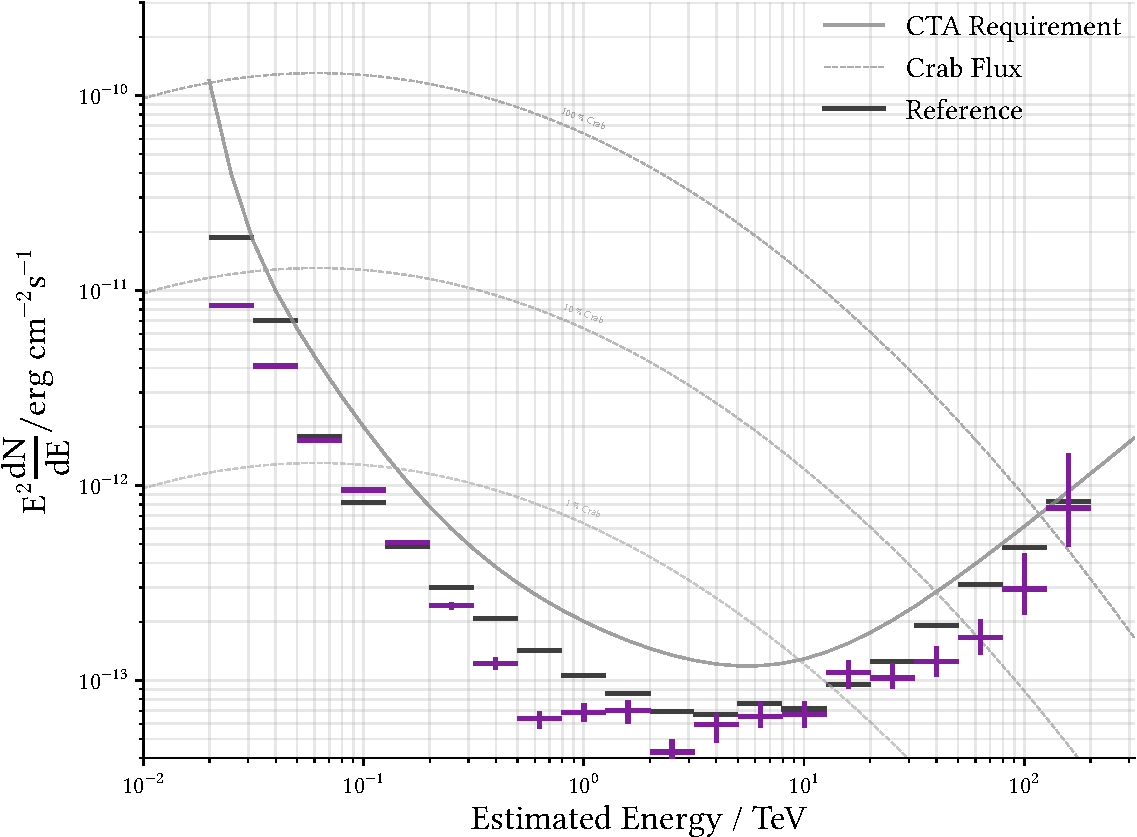
\includegraphics[width=0.6\textwidth]{../analysis/plots/sensitivity/hillas_sensitivity.pdf} 
    \caption{Computed sensitivity for the HillasReconstructor analysis against estimated event energy.
    The CTA requirements and
    reference results are added although a direct comparison is difficult. It can be noted though, that
    the general trend matches the expected results with the best sensitivity in the range from
    \num{1} to \SI{10}{\tera\electronvolt}. At high energies the uncertainties are increasing due to the low
    background statistic.}
    \label{fig:hillas_sens}
\end{figure}

With the cuts from the sensitivity optimisation, the effective area and angular resolution can be
compared as well.

The effective area, shown in figure \ref{fig:hillas_area}, exceeds the reference.
The angular resolution on the signal events, displayed in figure \ref{fig:hillas_resol}, is illustrated without
the $\Theta$ cuts to show the quaity of the reconstruction after apllying the
other cuts.
The large effective area is probably connected with the simplified background model
and the absence of cuts at lower data levels, such as on the number of pixels or
leakage, in this analysis.
At the same time the background counts in this analysis are already very low at high energies.
This leads to the conclusion, that the available statistic is just not sufficient
to get to any quantitative conclusions at high energies.

\begin{figure}
    \centering
    \captionsetup{width=0.9\linewidth}
    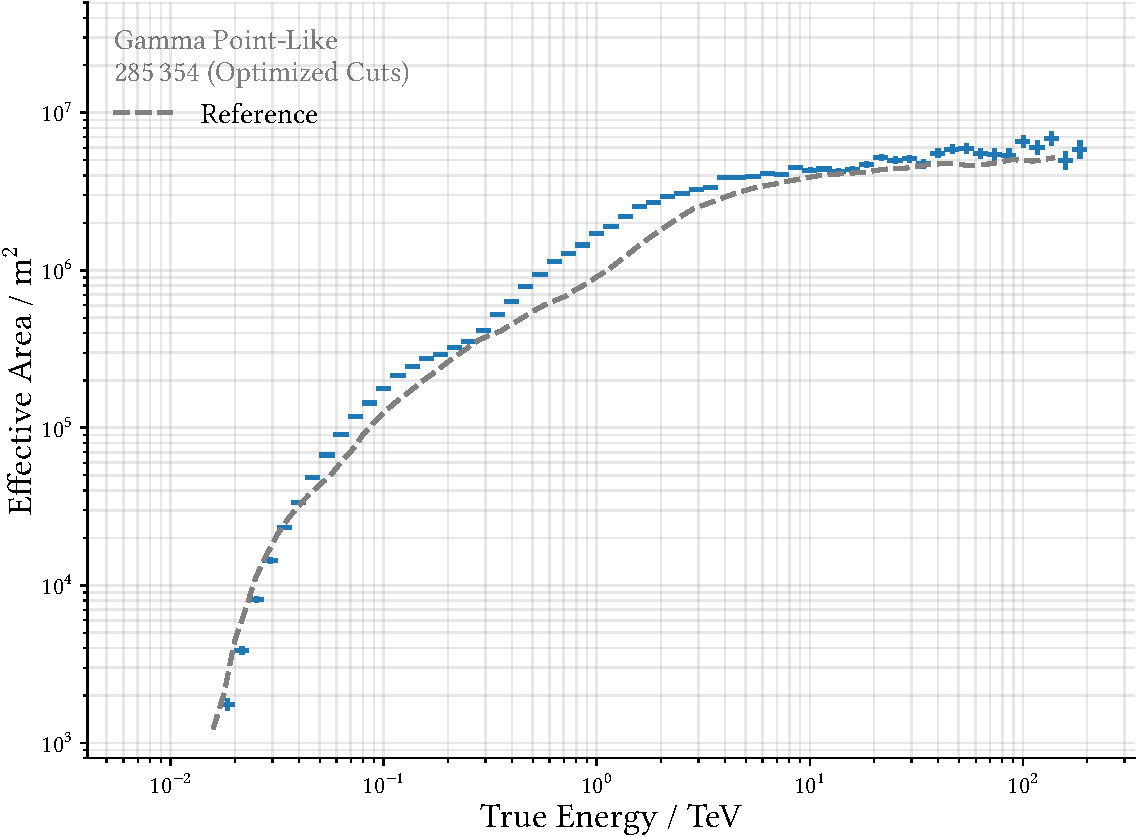
\includegraphics[width=0.6\textwidth]{../analysis/plots/sensitivity/hillas_effective_area.pdf} 
    \caption{Effective area against true event energy for the HillasReconstructor analysis
    with the pointlike gamma events after apllied cuts.
    As no cuts on the low level data have been performed and the high level cuts are relatively
    soft due to the low background event counts, the effective area is bigger at most energies.}
    \label{fig:hillas_area}
\end{figure}

\begin{figure}
    \centering
    \captionsetup{width=0.9\linewidth}
    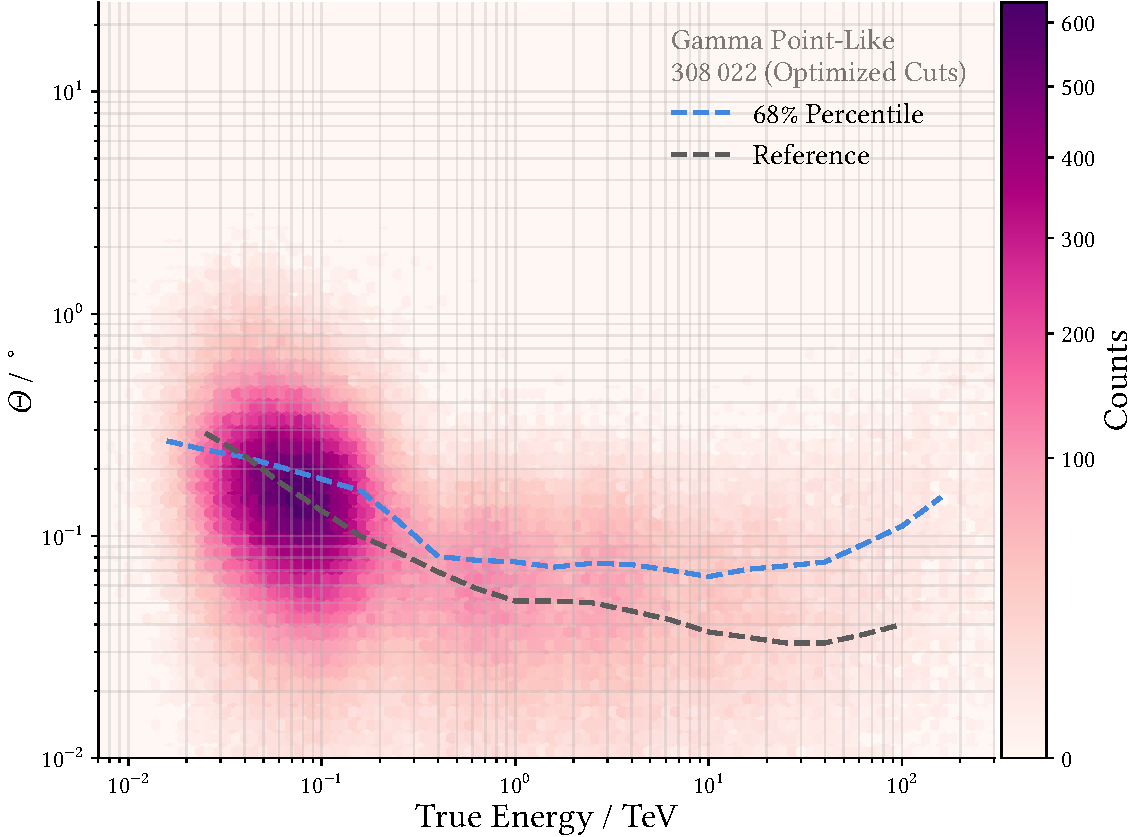
\includegraphics[width=0.6\textwidth]{../analysis/plots/sensitivity/hillas_resolution.pdf} 
    \caption{Angular resolution against true event energy after applied 
    prediction and multiplicity cuts for the HillasReconstructor analysis.
    For better illustration the colorbar has been scaled to account for the
    low event counts at high energies and no $\Theta$ cut is applied.}
    \label{fig:hillas_resol}
\end{figure}

Performing a grid search for the DISP analysis yields very similar cuts
in the prediction threshold and multiplicity (see table \ref{tab:disp_cuts}).
The direction cuts on the other hand are softer for high energies,
the total event counts are then once again comparable.

\newpage
\KOMAoption{paper}{landscape}
\areaset{2\textwidth}{.9\textheight}
\recalctypearea
    \centering
    \begin{tabular}{c c c c c r c c}
        %\hline
        $E_\text{min}$ / \si{\tera\electronvolt} & $E_\text{max}$ / \si{\tera\electronvolt} & $\alpha$ & $\Theta$ & Mult. & Sign. & sig counts & bkg counts \\
        \hline
        \num{0.02} & \num{0.03} & 0.75 & 0.15 & 2 & \num{85.30} & \num{19993.86} (\num{4924}) & \num{192060.04} (\num{466})\\
        \num{0.03} & \num{0.05} & 0.6 & 0.17 & 2 & \num{171.82} & \num{69965.93} (\num{16658}) & \num{562911.14} (\num{1183}) \\
        \num{0.05} & \num{0.08} & 0.6 & 0.17 & 2 & \num{388.16} & \num{200432.42} (\num{46953}) & \num{760783.92} (\num{2001}) \\
        \num{0.08} & \num{0.12} & 0.65 & 0.15 & 2 & \num{495.51} & \num{166607.87} (\num{39931}) & \num{207045.76} (\num{841}) \\
        \num{0.13} & \num{0.20} & 0.7 & 0.11 & 6 & \num{396.09} & \num{56680.18} (\num{14287}) & \num{10013.58} (\num{85}) \\
        \num{0.20} & \num{0.32} & 0.8 & 0.10 & 6 & \num{293.67} & \num{25293.69} (\num{7069}) & \num{499.86} (\num{6}) \\
        \num{0.32} & \num{0.50} & 0.8 & 0.08 & 10 & \num{264.91} & \num{19863.06} (\num{6275}) & \num{84.86} (\num{2}) \\
        \num{0.50} & \num{0.80} & 0.8 & 0.08 & 6 & \num{290.82} & \num{32776.77} (\num{9031}) & \num{46.86} (\num{2}) \\
        \num{0.80} & \num{1.26} & 0.8 & 0.08 & 7 & \num{235.79} & \num{15656.71} (\num{7354}) & \num{39.47} (\num{2}) \\
        \num{1.26} & \num{2.00} & 0.75 & 0.08 & 10 & \num{191.49} & \num{10300.78} (\num{6073}) & \num{17.79} (\num{1}) \\
        \num{2.00} & \num{3.17} & 0.75 & 0.09 & 6 & \num{184.62} & \num{9562.36} (\num{7745}) & \num{12.82} (\num{1}) \\
        \num{3.17} & \num{5.02} & 0.7 & 0.08 & 7 & \num{134.23} & \num{5091.10} (\num{5647}) & \num{18.62} (\num{3}) \\
        \num{5.02} & \num{7.96} & 0.7 & 0.08 & 9 & \num{91.14} & \num{2340.08} (\num{3701}) & \num{6.14} (\num{1}) \\
        \num{7.96} & \num{12.62} & 0.7 & 0.09 & 6 & \num{76.08} & \num{1632.71} (\num{3885}) & \num{4.97} (\num{1}) \\
        \num{12.62} & \num{20.00} & 0.65 & 0.08 & 10 & \num{41.84} & \num{500.16} (\num{1839}) & \num{3.91} (\num{1}) \\
        \num{20.00} & \num{31.70} & 0.6 & 0.1 & 5 & \num{36.38} & \num{379.53} (\num{2176}) & \num{3.54} (\num{1}) \\
        \num{31.70} & \num{50.24} & 0.6 & 0.1 & 2 & \num{23.86} & \num{170.69} (\num{1606}) & \num{5.40} (\num{3}) \\
        \num{50.24} & \num{72.62} & 0.45 & 0.12 & 4 & \num{15.90} & \num{77.76} (\num{1232}) & \num{3.64} (\num{1}) \\
        \num{79.62} & \num{126.19} & 0.45 & 0.11 & 2 & \num{8.36} & \num{24.45} (\num{685}) & \num{3.59} (\num{2}) \\
        \num{126.19} & \num{200.00} & 0 & 0.01 & 2 & \num{0.32} & \num{0.27} (\num{14}) & \num{2.43} (\num{1}) \\
    %\hline
    \end{tabular}
\clearpage
\newpage
% \KOMAoptions{paper=portrait,pagesize}
% \recalctypearea
\normalsetting

The resulting instrument response functions can be seen in figures
\ref{fig:disp_sens}, \ref{fig:disp_area} and \ref{fig:disp_resol}.
At energies up to a few \si{\tera\electronvolt} the effective area is slightly larger, 
for higher energies it falls off.
This is in line with the worse resolution at high energies, that was
previously displayed.
The angular resolution is very much identical, but
the event counts at high energies are lower as also shown by the effective area.

In comparison to the HillasReconstructor analysis, the sensitivity
is slighty improved for event energies under \SI{100}{\giga\electronvolt} and 
worse above.


\begin{figure}
    \centering
    \captionsetup{width=0.9\linewidth}
    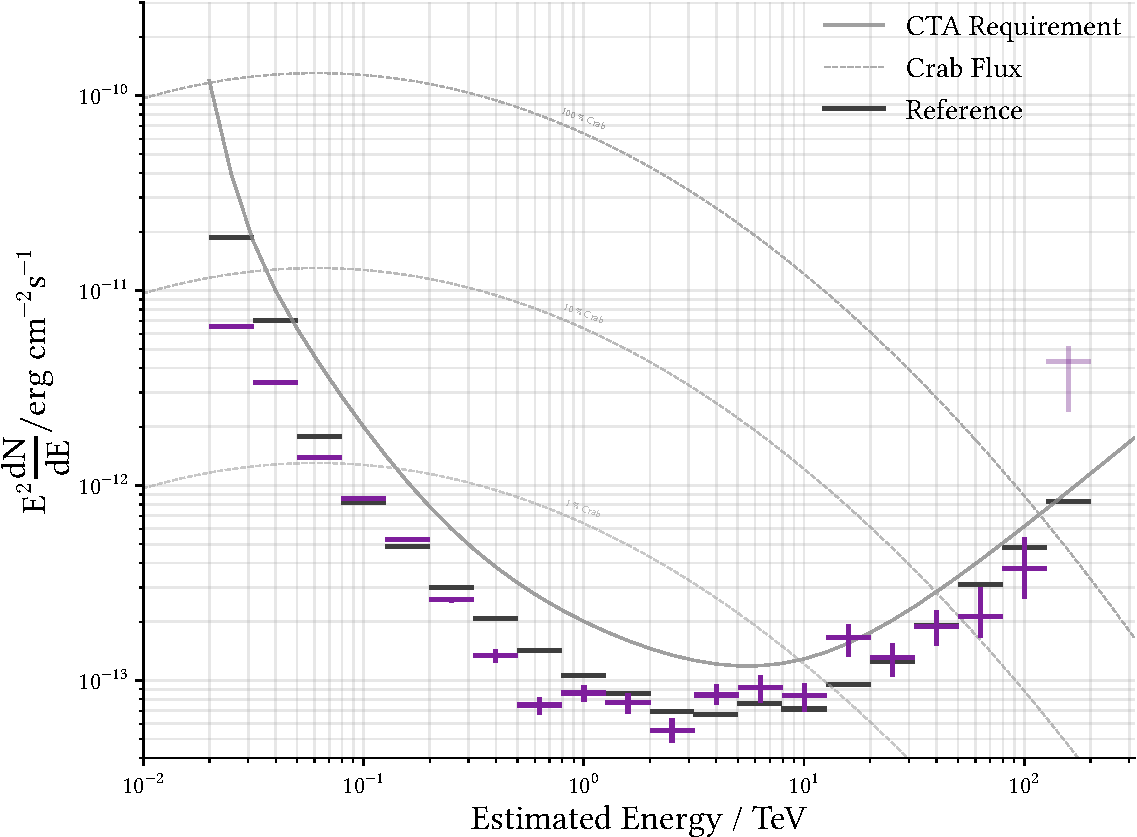
\includegraphics[width=0.6\textwidth]{../analysis/plots/sensitivity/disp_sensitivity.pdf} 
    \caption{Computed sensitivity for the HillasReconstructor analysis against estimated event energy.
    In comparison to the HillasReconstructor analysis, the results at the low energy bins are slightly
    superiour under \SI{100}{\giga\electronvolt} and worse
    above \SI{1}{\tera\electronvolt}.
    Similar conclusions regarding the background statistic and uncertainties
    at high energies can be drawn.}
    \label{fig:disp_sens}
\end{figure}

\begin{figure}
    \centering
    \captionsetup{width=0.9\linewidth}
    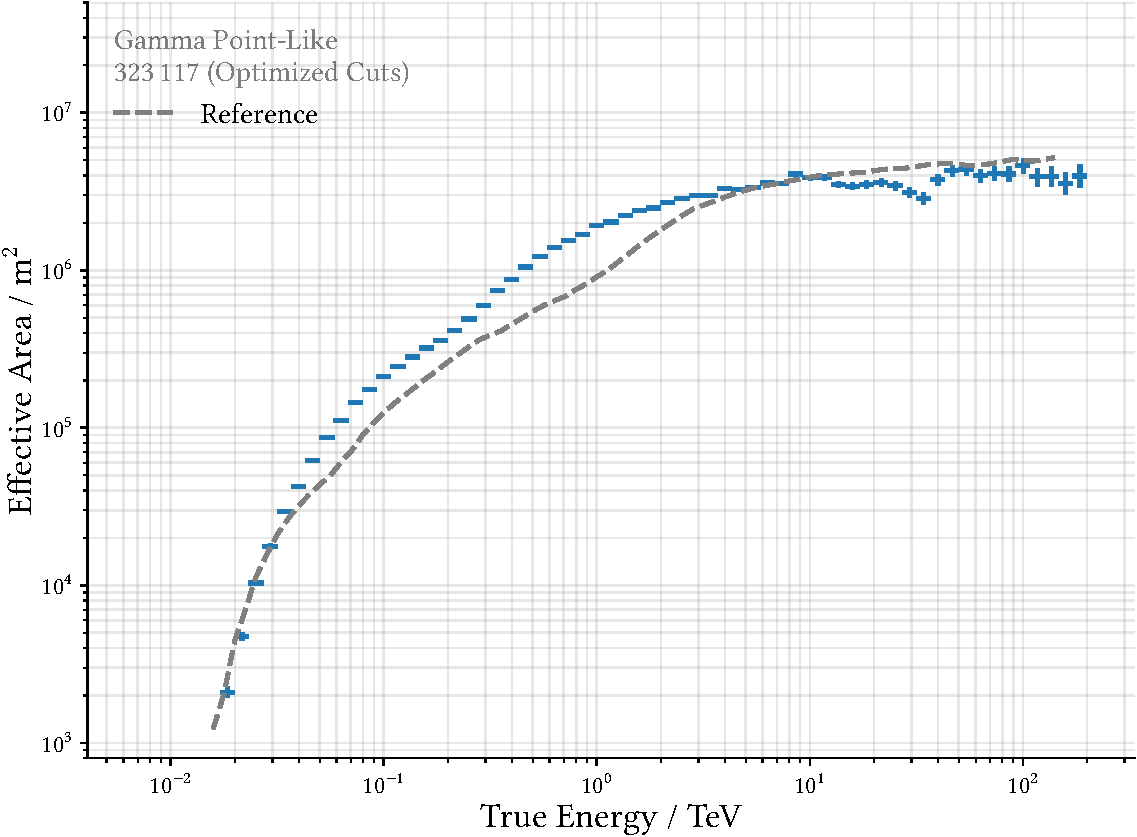
\includegraphics[width=0.6\textwidth]{../analysis/plots/sensitivity/disp_effective_area.pdf} 
    \caption{Effective area against true event energy for the DISP analysis
    with the pointlike gamma events after apllied cuts.
    The effective area is even larger for low and mid energies compared 
    to the previous HillasReconstructor results, but falls short above
    $\SI{10}{\tera\electronvolt}$.}
    \label{fig:disp_area}
\end{figure}

\begin{figure}
    \centering
    \captionsetup{width=0.9\linewidth}
    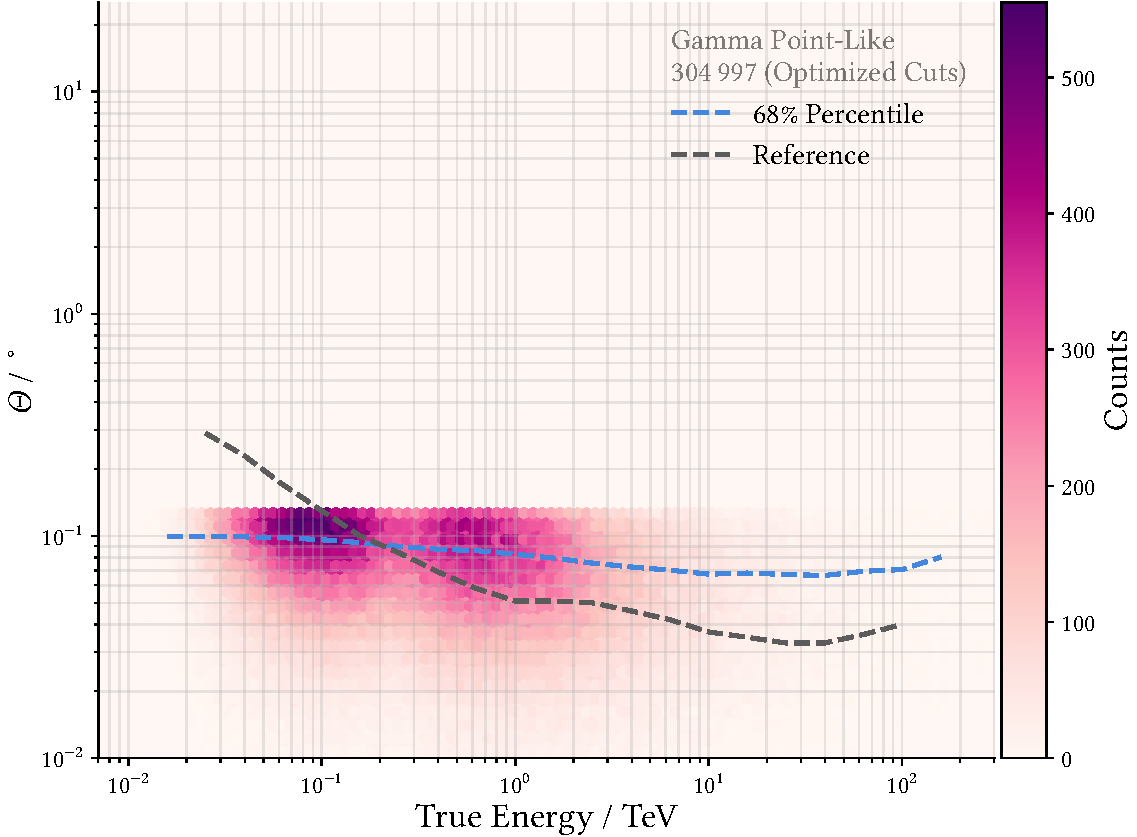
\includegraphics[width=0.6\textwidth]{../analysis/plots/sensitivity/disp_resolution.pdf} 
    \caption{Angular resolution against true event energy after applied 
    prediction and multiplicity cuts for the DISP analysis.
    For better illustration the colorbar has been scaled to account for the
    low event counts at high energies and no $\Theta$ cut is applied.}
    \label{fig:disp_resol}
\end{figure}
% 
\chapter{Conclusion and Outlook}
\label{conclusion}

\section{Conclusion}
In the course of this work, analyis methods for CTA data have been tested.
As CTA is still in construction, the analysis is limited on the use of monte carlo data.

The necessary steps to go from low level CTA-data to a high-level analysis have been performed
using the official analysis pipeline ctapipe, that is still actively being developed.
A high-level reconstruction based on the use of random forests 
and the aict-tools package has been worked out as alternative
or complement to the existing algorithms.
Diffuse proton and gamma simulations have been used as training samples for the models, 
whereas the evaluation was done on pointlike gamma samples.

With this setup, gamma-/hadron separation works as expected and different algorithms 
for the source position reconstruction lead to roughly comparable angular
resolutions.
Due to the layout of the CTA (south) array, low energy events, on average, have lower multiplicities.
This makes is difficult to reconstruct the source position with the HillasReconstructor 
algorithm and a DISP-based approach can lead to improvements. This is especially true for
event multiplicities two or three and can thus be relevant for the early stages of operation of CTA.
At high event energies and high multiplicities, the HillasReconstructor is unrivaled.

A simplified sensitivity optimisation for both methods has been performed with
the same results regarding the performance in different energy bins.
As most parts of the analysis were the same for both methods, the results
are very similar.
An in depth comparison to the reference analysis of CTA is not feasible,
but the sensitivity seems to be not too far off.
The effective area is larger, whereas the angular separation is worse,
which points towards harder cuts - maybe also in earlier analysis steps - 
in the reference analysis.

\section{Outlook}
A lot of potential to improve the analysis is still open:

The performed preprocessing uses a rather generic cleaning, with
parameters, that were generally accepted as being 
decent, but not overly optimised in the working group. Recently, 
more relaxed parameters - especially for the LSTCam - have been used.
Furthermore, more complex cleaning methods could be inspected further.
Since the start of this thesis, two additional algorithms have been 
implemented into ctapipe:
An imcomplete three-threshold procedure used in CTA-MARS, which does not factor 
in timing information yet, and a procedure used in the FACT experiment.
The last one was added to ctapipe by me, but due to the high effort to
optimize the cleaning parameters, was not used for the analysis.
Additionaly, no cuts have been performed on the data apart from
the high level sensitivity cuts. Disregarding hard to reconstruct
events, such as events with high leakage or low intensity,
could further improve the analysis.

In the foreseeable future, new monte carlo data will be accesible as well.
This dataset will act as a common benchmark dataset in the collaboration,
which makes comparing results and optimizing parameters easier.

Future steps could also include an analysis of observed monoscopic 
LST data. Since the LST is currently the only telescope 
at LaPalma, an analysis can not rely on stereoscopic information.
The methods employed for the background separation, energy estimation and 
DISP-calculation will also work in the purely monoscopic case, although further
optimisation will probably be needed.

At last all models could be optimized in terms of the used architecture and
hyper parameters. Although random forests are generally 
robust in terms of the used hyper parameters, some gains might still be 
open. 
A recent thesis at this chair for example was based on using
extremely randomized trees for the models.
Earlier work has also shown, that an approach with two nested models
can be superiour for the energy estimation. In that case
a random forest model was trained on telescope level and
a second randm forest combined these results using the
array wide features and the combined predictions \cite{ba-lars}.
These results have been verified during the course of this thesis,
but the focus was put on the DISP based reconstruction of the
source position.

\newpage
\appendix
%Hier beginnt der Anhang, nummeriert in lateinischen Buchstaben
\chapter{Parameters}
\label{sec:app_params}

config kram hier hin


\backmatter
\printbibliography



\cleardoublepage
\includepdf[pages=-]{eidesstattliche_versicherung.pdf}
% \thispagestyle{empty}
\section*{Eidesstattliche Versicherung}
Ich versichere hiermit an Eides statt, dass ich die vorliegende Abschlussarbeit mit dem Titel \enquote{\thetitle} selbstständig und ohne unzulässige fremde Hilfe erbracht habe.
Ich habe keine anderen als die angegebenen Quellen und Hilfsmittel benutzt, sowie wörtliche und sinngemäße Zitate kenntlich gemacht. 
Die Arbeit hat in gleicher oder ähnlicher Form noch keiner Prüfungsbehörde vorgelegen.

\vspace*{1cm}\noindent
\begin{center}
  \begin{tabular}{@{}p{0.4\textwidth}@{\hspace{0.15\textwidth}}p{0.4\textwidth}@{}}
  \rule{\linewidth}{0.25pt}& \rule{\linewidth}{0.25pt}\\
  Ort, Datum & Unterschrift
  \end{tabular}
\end{center}

\subsection*{Belehrung}
Wer vorsätzlich gegen eine die Täuschung über Prüfungsleistungen betreffende Regelung einer Hochschulprüfungsordnung verstößt, handelt ordnungswidrig.
Die Ordnungswidrigkeit kann mit einer Geldbuße von bis zu \SI[round-mode=places, round-precision=2]{50000}{€} geahndet werden. 
Zuständige Verwaltungsbehörde für die Verfolgung und Ahndung von Ordnungswidrigkeiten ist der Kanzler/die Kanzlerin der Technischen Universität Dortmund. 
Im Falle eines mehrfachen oder sonstigen schwerwiegenden Täuschungsversuches kann der Prüfling zudem exmatrikuliert werden \mbox{(\S\,63 Abs. 5 Hochschulgesetz --HG--).}

Die Abgabe einer falschen Versicherung an Eides statt wird mit Freiheitsstrafe bis zu 3 Jahren oder mit Geldstrafe bestraft.

Die Technische Universität Dortmund wird ggf.\ elektronische Vergleichswerkzeuge (wie z.\,B.\ die Software \enquote{turnitin}) zur Überprüfung von Ordnungswidrigkeiten in Prüfungsverfahren nutzen. \\[\baselineskip]

\noindent Die oben stehende Belehrung habe ich zur Kenntnis genommen.\\[1cm]
\begin{center}
\begin{tabular}{@{}p{0.4\textwidth}@{\hspace{0.15\textwidth}}p{0.4\textwidth}@{}}
\rule{\linewidth}{0.25pt}& \rule{\linewidth}{0.25pt}\\
Ort, Datum & Unterschrift
\end{tabular}
\end{center}

\end{document}
